\documentclass[10pt]{article}
\usepackage{geometry}                % See geometry.pdf to learn the layout options. There are lots.
\geometry{letterpaper}                   % ... or a4paper or a5paper or ... 
%\geometry{landscape}                % Activate for for rotated page geometry
%\usepackage[parfill]{parskip}    % Activate to begin paragraphs with an empty line rather than an indent

%%%%%%%%%%%%%%%%%%%%
\newcommand{\hide}[1]{}

\usepackage{natbib}
\usepackage{xcolor}
\usepackage{url}
\usepackage{hyperref}
\usepackage{mathtools}
\usepackage{enumerate}
\usepackage{amsmath}
\usepackage{amssymb}

\hide{
\usepackage{amscd}
\usepackage{amsfonts}
\usepackage{amsmath}
\usepackage{amssymb}
\usepackage{amsthm}
\usepackage{cases}		 
\usepackage{cutwin}
\usepackage{enumerate}
\usepackage{epstopdf}
\usepackage{graphicx}
\usepackage{ifthen}
\usepackage{lipsum}
\usepackage{mathrsfs}	
\usepackage{multimedia}
\usepackage{wrapfig}
}

\usepackage{commath}
\usepackage{cancel}
\usepackage{systeme}
\usepackage{graphicx}
\usepackage{sgame}
\usepackage{listings}
\usepackage{etoolbox}
\usepackage[shortlabels]{enumitem}



\bibliographystyle{humanbio}
\setcitestyle{square}

\usepackage{enumitem}% http://ctan.org/pkg/enumitem

\usepackage{tikz-cd}


	 
%\input{/usr/local/LATEX/Lee_newcommands.tex}




%index commands
\newcommand{\ri}{j}
\newcommand{\hi}{i}

\usepackage{amsthm}

\theoremstyle{plain}
\newtheorem{thm}{Theorem}[section] % reset theorem numbering for each chapter
\newtheorem{theorem}{Theorem}[section]
\newtheorem{corollary}[thm]{Corollary}
\newtheorem{lemma}[thm]{Lemma}
\newtheorem{prop}[thm]{Proposition}


\theoremstyle{definition}
\newtheorem{defn}[thm]{Definition} % definition numbers are dependent on theorem numbers
\newtheorem{exmp}[thm]{Example} % same for example numbers
\newtheorem{exercise}[thm]{Exercise}
\AfterEndEnvironment{defn}{\noindent\ignorespaces}
\AfterEndEnvironment{exmp}{\noindent\ignorespaces}
\AfterEndEnvironment{prop}{\noindent\ignorespaces}
\AfterEndEnvironment{proof}{\noindent\ignorespaces}
\AfterEndEnvironment{theorem}{\noindent\ignorespaces}
\AfterEndEnvironment{thm}{\noindent\ignorespaces}


\newenvironment{semiproof}{\textit{Semi-Proof:}}{\hfill$\square$}
\newenvironment{subproof}{\textit{Subproof:}}{\hfill$\square$}

\usepackage{pythonhighlight} %https://github.com/olivierverdier/python-latex-highlighting/blob/master/pythonhighlight.sty
\colorlet{commentcolour}{gray}
\colorlet{stringcolour}{green!50!black}
\colorlet{keywordcolour}{blue!80!black}
\colorlet{exceptioncolour}{yellow!50!red}
\colorlet{commandcolour}{blue!60!black}
\colorlet{numpycolour}{blue!60!green}
\colorlet{literatecolour}{black}
\colorlet{promptcolour}{orange}
\colorlet{specmethodcolour}{violet}

\colorlet{otherkeywords}{orange}

\usepackage{nccmath}
\usepackage{graphicx}
\graphicspath{ {./graphics/} }
\usepackage{caption}

\usepackage[
backend=biber,
style=alphabetic,
sorting=ynt
]{biblatex}
\addbibresource{mybibliography.bib}

\usepackage{titletoc}



\def\labelitemi{--} %gets itemize looking the way I want
\setcounter{section}{-1} %starts indexing of sections from 0
%\renewcommand{\thesection}{} %gets rid of them alltogether




\newcommand{\itemlist}[1]{\begin{itemize}#1\end{itemize}}
\newcommand{\enumlist}[1]{\begin{enumerate}#1\end{enumerate}}
\newcommand{\desclist}[1]{\begin{description}#1\end{description}}

\newcommand{\Answer}[1]{\begin{quote}{\color{blue}#1}\end{quote}}
\newcommand{\AND}{\wedge}
\newcommand{\OR}{\vee}
\newcommand{\ra}{\rightarrow}
\newcommand{\lra}{\leftrightarrow}

\usepackage{ifthen}



%%%   WORD DEFINITIONS
\newcommand{\with}{\text{ with }}
\newcommand{\where}{\text{ where }}
\newcommand{\myand}{\text{ and }}
\newcommand{\st}{\text{ s.t. }}
\newcommand{\myif}{\text{ if }}
\newcommand{\ie}{\text{ i.e. }}


\newcommand{\Recall}{\textbf{Recall: }}
\newcommand{\Notation}{\textbf{Notation: }}
\newcommand{\Note}{\textbf{Note: }}
\newcommand{\KeyPoint}{\textbf{Key Point: }}
\newcommand{\Claim}{\textbf{Claim: }}
\newcommand{\Fact}{\textbf{Fact: }}


\newcommand{\id}{\text{id}}

\newcommand{\Real}{\mathbb{R}}
\newcommand{\man}{\mathcal{M}}
\newcommand{\nan}{\mathcal{N}}
\newcommand{\pan}{\mathcal{P}}

\newcommand{\chartU}{\mathcal{U}}
\newcommand{\chartV}{\mathcal{V}}
\newcommand{\chart}{\varphi}
\newcommand{\varchart}{\psi}
\newcommand{\Atlas}{\mathcal{A}}
\newcommand{\alphaatlas}{\left\{(\chartU_\alpha,\chart_\alpha)\right\}}
\newcommand{\varalphaatlas}{\left\{(\chartV_\alpha,\varchart_\alpha)\right\}}
\newcommand{\trans}{\tau_{\alpha\beta}}

\newcommand{\xman}{x\in\man}

\newcommand{\setform}[2]{\Lambda^{#1} {#2}}
\newcommand{\Hom}[2]{\text{Hom}\left(#1,#2\right)}
\newcommand{\HomReal}[2]{\text{Hom}_\Real\left(#1,#2\right)}

\newcommand{\allthevs}[2]{v_{#1},...,v_{#2}}
\newcommand{\allthe}[3]{{#1}_{#2},...,{#1}_{#3}}
\newcommand{\wedgge}{\omega_1\wedge\omega_2}
\newcommand{\allthewedge}[3]{{#1}_{#2}\wedge...\wedge{#1}_{#3}}

\newcommand{\tang}{T_x\man}
\newcommand{\dualtang}{T_x^*\man}

\newcommand{\tangbundle}{T\man}
\newcommand{\dualtangbundle}{T^*\man}

\newcommand{\difftang}{\setform{p}{\dualtang}}
\newcommand{\difftangbundle}{\setform{p}{T^*M}}
\newcommand{\pdifftangbundle}[1]{\setform{#1}{T^*M}}

\newcommand{\pformman}[1]{\Omega^{#1}(\man)}
\newcommand{\pformnan}[1]{\Omega^{#1}(\nan)}

\newcommand{\compactpformman}[1]{\Omega^{#1}_c(\man)}
\newcommand{\compactpformnan}[1]{\Omega^{#1}_c(\nan)}


\newcommand{\manforms}{\Omega^\bullet(\man)}

\newcommand{\tangof}[1]{T_x[#1]}
\newcommand{\iparderiv}[1]{\frac{\partial}{\partial x_{#1}}}
\newcommand{\iparderivof}[2]{\frac{\partial {#2}}{\partial x_{#1}}}
\newcommand{\dx}{dx}
\newcommand{\dy}{dy}
\newcommand{\dz}{dz}
\newcommand{\deriv}{d}
\newcommand{\df}{df}
\newcommand{\dw}{d\omega}
\newcommand{\deta}{\deriv\eta}
\newcommand{\dt}{\deriv t}


\newcommand{\cts}[1]{\mathcal{C}^{\infty}(#1)}

\newcommand{\sumfromto}[2]{\sum\limits_{#1}^{#2}}

\newcommand{\dwedgge}{\deriv\omega_1\wedge\deriv\omega_2}

\newcommand{\plusReal}{\Real_+ ^n}

\def\restrict#1{\raise-.5ex\hbox{\ensuremath|}_{#1}}


\DeclareMathOperator{\Ker}{Ker}
\DeclareMathOperator{\Ima}{Im}

\newcommand{\cohomman}[1]{H^{#1}(\man)}
\newcommand{\coZman}[1]{Z^{#1}(\man)}
\newcommand{\coBman}[1]{B^{#1}(\man)}
\newcommand{\cohomnan}[1]{H^{#1}(\nan)}
\newcommand{\coZnan}[1]{Z^{#1}(\nan)}
\newcommand{\coBnan}[1]{B^{#1}(\nan)}
\newcommand{\compactcohomman}[1]{H_c^{#1}(\man)}
\newcommand{\compactcohomnan}[1]{H_c^{#1}(\nan)}

\newcommand{\inter}{\left[0,1\right]}

\newcommand{\parderiv}[1]{\frac{\partial}{\partial {#1}}}

\newcommand{\impliesdirection}{\underline{\Rightarrow:}}
\newcommand{\impliedbydirection}{\underline{\Leftarrow:}}

\newcommand{\cochaincomplex}{\left(C^\bullet,d^\bullet\right)}
\newcommand{\varcochaincomplex}{\left(D^\bullet,d'^\bullet\right)}

\newcommand{\SES}[3]{0\to {#1}^\bullet \to {#2}^\bullet \to {#3}^\bullet \to 0}
\newcommand{\funcSES}[5]{0\to {#1}^\bullet \xrightarrow{#2} {#3}^\bullet \xrightarrow{#4} {#5}^\bullet \to 0}
\newcommand{\ABCSES}{\SES{A}{B}{C}}
\newcommand{\funcABCSES}{\funcSES{A}{f}{B}{g}{C}}

\newcommand{\UintV}{U\cap V}
\newcommand{\cohomUV}[1]{H^{#1}(U)\oplus H^{#1}(V)}
\newcommand{\cohom}[2]{H^{#1}(#2)}

\newcommand{\puncman}{\overset{\circ}{\man}}

\DeclareMathOperator{\rank}{rank}
\DeclareMathOperator{\sign}{sign}
\DeclareMathOperator{\supp}{supp }

\newcommand{\CProj}{\mathbb{CP}}
\newcommand{\remzero}{\backslash \{0\}}
\newcommand{\mycasesthing}[2]{\begin{cases} #1 \\ #2\end{cases}}
\DeclareMathOperator{\pt}{pt}

\DeclareMathOperator{\Eig}{Eig}

\newcommand{\tdiffof}[1]{\frac{\deriv #1}{\dt}}

















%%%%%%%%%%%%%%%%%%%%%%%%%%%%%%%%%%%%%%%%%%%%%%%

\title {Differential Topology\\Spring Term 2021\\
Preliminary Lecture Notes}
\author{Lectured by Dr Joshua Jackson at Imperial College London\\
Written by Jack Kennedy}
\date{}

\begin{document}
\maketitle
\tableofcontents
\newpage
$\textbf{DISCLAIMER}$: These notes are not yet finished. If you spot any typos or things I should include, please let me know at $\textit{jk3617@ic.ac.uk}$. All mathematical content and proofs are provided by Dr Jackson, and these notes try their best to capture exactly what he wrote during lectures. That said, any jokes, strange remarks or quips are, unfortunately, mine and made in a attempt to keep myself sane while crying over why my LaTeX won't compile.

\begin{section}{Lecture 0: Welcome, Admin, Course Overview}
{Goals of different flavours of Topology:}
\begin{enumerate}
    \item Classical Topology : Classify all topological space up to homeomorphism 
    \begin{enumerate}[]
        \item Problem: Too ambitious, very very difficult
    \end{enumerate}
    \item Algebraic Topology: Assign simple algebraic invariants to topological spaces, e.g. finitely generated Abelian group 
    \begin{enumerate}
        \item Fundamental Group $\pi_1(X)$: from homotopy classes of cts maps ${S}^1 \to X$
        \item Higher homotopy groups $\pi_k(X)$: from homotopy classes of cts maps $S^k \to X$
        \item[] Problem: Phenomenally hard to compute for general $k$, even for simple spaces like $S^n$
        \item Singular homology groups $H_k(X)$: defined via homotopy from $\bigtriangleup^k \to X $, plus some homological algebra (Fundamental group detects 1D holes in $X$, homological groups does it for higher D)
        \item Singular cohomology groups: dual to homology groups, has a ring structure, $\bigoplus\limits_
        k H^k(X)$ is a ring.
        \item Betti numbers: $b_k(X) \coloneqq \text{Rk} H_k(X) = \text{Rk} H^k(X)$
    \end{enumerate}
    \item[] All of these are invariant under homotopy, and they're also functorial! i.e. map $f : X\to Y$ of top. spaces gives a map (e.g. grp homo, ring homo.) of the corresponding invariants, so like a $f^* : X^* \to Y^*$ where $X^*$ is some associated space like the fundamental group. 
    \item Differential Topology: Focus on smooth manifolds, particularly nice spaces where you can ``do calculus". 
\end{enumerate}
\Recall A smooth manifold is a second countable Hausdorff space $\mathcal{M}$, equipped with a maximal smooth atlas (or smooth structure) $\mathcal{A} = \{(\mathcal{U}_{\alpha},\varphi_{\alpha})\}_{\alpha} $ i.e.
\begin{enumerate}[(i)]
    \item $\mathcal{U}_{\alpha}$ form an open cover of $\mathcal{M}$
    \item $\varphi_{\alpha} : \chartU_{\alpha} \to \varphi_{\alpha}(\mathcal{U}_{\alpha}) \subseteq \Real^n$ homeomorphism onto its image
    \item Transition maps $\tau_{\alpha\beta} \coloneqq \chart_{\beta} \circ \chart_{\alpha}^{-1} : \chart_{\alpha}(\chartU_{\alpha}\cap\chartU_{\beta}) \to \chart_{\beta}(\chartU_{\alpha}\cap\chartU_{\beta}) \subseteq \Real^n$ are all diffeomorphisms. Sufficient to ask all partial derivatives of all orders to be smooth.
    \item $\Atlas$ is maximal: if $\chart_{\beta} : \chartU_{\beta} \to \Real^n$ is another coordinate chart compatible with $\Atlas$, in the sense that $\chart_{\beta} \circ \chart_{\alpha} ^{-1}$ is a diffeomorphism for all charts $\chart_{\alpha}$ in $\Atlas$, then $(\chartU_{\beta},\chart_{\beta}) \in \Atlas$. 
\end{enumerate}
In this course: versions of (co)homology for smooth manifolds. \\Questions we'll ask:
\begin{enumerate}
    \item What's special about invariants of smooth manifolds?\\ E.g. Poincar\'e Duality: If $\man$ compact oriented smooth manifold, then $H^k(\man) \cong H_{n-k}(\man)$ where dim $\man = n$, so in particular $b_k(\man) = b_{n-k}(\man)$
    \item Can we interpret invariants, and the algebraic structures on them in a (differential) geometric way? \begin{itemize}
        \item  de Rham Cohomology: defined from differential forms on $\man$ yields same groups as singular cohomology. Interpreting topological information via something to do with solvability of differential eq$^n$s on $\man$
        \item  Degrees of smooth maps between manifolds: $F : \man\to\nan$ compact oriented manifolds of dim $n$, then corresponding morphism $F^* : H^n(\nan)\to H^n(\man)$ can be interpreted as ``number of preimages of a `generic' point $x\in \nan$ (counted with signs)''.
        \item Morse Theory: can recover homology of $\man$ from data of `morse function' $f : \man \to \Real$ smooth with non-degenerate critical points.
    \end{itemize}
\end{enumerate}
\textbf{References}:\\
Main Ones:
\begin{enumerate}
    \item John Lee, Introduction to Smooth Manifolds
    \item L. Tu, An Introduction to Manifolds
\end{enumerate}
Other Ones:
\begin{enumerate}
  \setcounter{enumi}{3}
    \item J. Milnor, Morse Theory
    \item Hatcher, Algebraic Topology, Chapters 2 \& 3 (useful for singular homology)
\end{enumerate}
\noindent
\textbf{Outline of Course:}
\begin{enumerate}
    \item Differential Forms on Manifolds:
    \begin{itemize}
        \item Integration of differential forms
        \item Exterior derivative
        \item Stokes' theorem and applications
    \end{itemize}
    \item de Rham Cohomology:
    \begin{itemize}
        \item Homotopy invariance
        \item Mayer-Vietoris
        \item Poincar\'e duality
        \item The Künneth formula
        \item Degree of a morphism
    \end{itemize}
    \item Morse Theory (``Homology theory for Smooth Manifolds'')
    \begin{itemize}
        \item CW complexes
        \item Fundamental theorems of Morse theory
    \end{itemize}
    \item Singular homology and cohomology
    \begin{itemize}
        \item de Rham theorem (``secretly studying [algebraic topology] all along'')
    \end{itemize}
\end{enumerate}
\end{section}

\begin{section}{Lecture 1: Prelude on Multi-Linear Algebra}
Let $V$ be a real vector space of dimension $n$. Let $p\geq0$. Write $V^p = V\times ...\times V$, $p$ times.
\begin{defn}
A multi-linear function $\omega : V^p \to \Real$ is called an \textbf{alternating $p$-form} iff $\forall \sigma\in S_p, \forall v_1,...v_p \in V,$ $$\omega(v_{\sigma(1)},...,v_{\sigma(p)}) = \epsilon(\sigma) (v_1,...,v_p)$$
where $\epsilon(\sigma)$ is the sign of $\sigma$, i.e. $(-1)^m$ where $m$ is the number of transpositions in a decomposition of $\sigma$ in transpositions.
\end{defn}
\begin{exercise}
$\omega : V^p \to \Real$ is an alternating $p$-form iff $\forall i,j, \omega(v_1,...,v_i,...v_j,...v_p) =  -\omega(v_1,...,v_j,...,v_i,...,v_p)$ ($i^{th} \myand j^{th}$ places being swapped). In particular if $v_i = v_j$, $\omega(v_1,...,v_p) = 0$
\end{exercise}



\noindent
\Notation $\Lambda^p V^* = \{$alternating $p$-forms on $V\}$
\begin{exercise}
$\wedge^p V^*$ is a vector space.
\end{exercise}
\begin{exmp}
 (i) $\Lambda^0 V^* = \Real$ \quad (ii) $\Lambda^1V^* = V^* \coloneqq \Hom{V}{\Real}$
\end{exmp}
\begin{defn}
Let $\omega_1 \in \setform{p}{V^*}, \omega_2 \in \setform{q}{V^*}$. The \textbf{exterior product}, or wedge product $\omega_1~\wedge~\omega_2~\in~\setform{p+q}{V^*}$ is defined by
$$\omega_1\wedge\omega_2 \coloneqq \sum\limits_{\sigma \in S_{p,q}}\epsilon(\sigma)\, \omega_1(\allthevs{\sigma(1)}{\sigma(p)})\,\omega_2(\allthevs{\sigma(p+1)}{\sigma(p+q)})$$
for all $\allthevs{1}{p+q}$, and where $ S_{p,q} \coloneqq \{ \sigma \in S_{p+q} : \sigma(1)<...<\sigma(p),\sigma(p+1)<...<\sigma(p+q)\} $, the group of $(p,q)$ shuffles,  ``a deck of $p+q$ cards split into a pile of $p$ and $q$ stacks, and then riffle shuffled together''.
\end{defn}
\begin{prop}
Let $\omega_i \in \setform{p_i}{V^*}$ for $i = 1,2,3$. We have:
\begin{enumerate}[(i)]
    \item (Associativity) $(\omega_1\wedge\omega_2)\wedge\omega_3 =\omega_1\wedge(\omega_2\wedge\omega_3 ) $
    \item (Distributivity) $\omega_1\wedge(\omega_2+ \omega_3) = \omega_1\wedge\omega_2 + \omega_1\wedge\omega_3,\quad$ when $p_2 = p_3$
    \item (Supercommutativity) $\omega_1\wedge\omega_2 = (-1)^{p_1 p_2}\omega_2\wedge\omega_1$ 
\end{enumerate}
\end{prop}
\begin{proof}
All rather trivial and straight forward, see Manifolds notes.
\end{proof}
\begin{exmp}\noindent
\begin{enumerate}[($i$)]
    \item If $\omega_1,\omega_2 \in \setform{1}{V^*}$, then $\wedgge(v_1,v_2) =\omega_1(v_1)\omega_2(v_2) - \omega_2(v_1)\omega_1(v_2)$
    \item If $\omega_1,...,\omega_p \in \setform{1}{V^*},$ then for $\allthevs{1}{p}\in V$ $\omega_1\wedge...\wedge\omega_p(\allthevs{1}{p}) = \det(\omega_i(v_j))$, $i,j, = 1,...,p$.
\end{enumerate}
\end{exmp}
\begin{defn}
Let $\allthe{e}{1}{n}$ be a basis of $V$, and $\allthe{e^*}{1}{n}$ be the dual basis of $V^*$. For $I \subseteq \{1,...,n\} \st \vert I \vert = p$, define $\alpha_I = \allthewedge{e^*}{i_1}{i_p}$ where $I = \{\allthe{i}{1}{p}\}$ and $i_1 < ... < i_p$. Let $e_I = (\allthe{e}{i_1}{i_p})$. Then $\alpha_I(e_J) = \delta_{IJ} = \begin{cases} 
    0 &\myif I \neq J \\
    1 &\myif  I = J
\end{cases} $   because $\det$ = 1 if matrix is identity, 0 if the matrix is singular and index sets aren't equal.
\end{defn}
\begin{prop}
The alternating $p$-forms $\alpha_I$ are a basis for $\setform{p}{V^*}.$
\end{prop}
\begin{proof}
Linear independence: If $ \omega = \sum\limits_{I} c_I \alpha_I,$ for $c_I \in \Real$, then $\omega = 0 \implies \omega(e_I) = 0$ so that $ c_I = 0$ for all $I$.
Spanning: Let $\omega \in \setform{p}{V^*}$. Let $\omega'= \sum\limits_{I} \omega(e_I)\cdot \alpha_I$. Claim: $\omega' = \omega$. For all $I$ we have $(\omega-\omega')(e_I) =0$. Left as an exercise (Hint: use linearity and alternating property).
\end{proof}
\begin{corollary}
$\dim \setform{p}{V^*} = {\binom{n}{p}}$
\end{corollary}
\begin{exmp}
If $V = \Real^3$ then $\setform{2}{\Real^3} = \langle e^*_1 \wedge e_2^*,e^*_1 \wedge e_3^*,e^*_2 \wedge e_3^*\rangle$
\end{exmp}
\begin{defn}
Let $\Phi : V \to W$ be a linear map, and $\omega \in \setform{p}{W^*},$ then the \textbf{pullback} $\Phi^*\omega \in \setform{p}{V^*}$ is given by
$$\Phi^* \omega(\allthevs{1}{p}) = \omega(\Phi(v_1),...,\Phi(v_p)) $$
for $\allthevs{1}{p} \in V$
\end{defn}
\begin{prop}
The pullback of the linear function $\Phi:V\to W$ has the following properties:
\begin{enumerate}
    \item (Respects Wedge) $\omega_1 \in\setform{p}{W^*}, \omega_2\in\setform{q}{W^*} \implies \Phi^*(\wedgge) = \Phi^*(\omega_1)\wedge \Phi^*(\omega_2)$
    \item (Composition) If $\Psi:W\to Z$ linear, then $(\Psi\circ\Phi)^*\omega = \Phi^*\Psi^*\omega$
    \item If $V = W$, then $\Phi^*\omega = \det\Phi\cdot\omega$ for all $\omega \in \setform{p}{V^*}$
\end{enumerate}
\end{prop}
\end{section}
\begin{section}{Lecture 2: Differential Forms on Manifolds, and the Exterior Derivative}
Let $\man $ be a smooth manifold of dimension $n$. For $\xman$, recall $T_x\man$, the tangent space to $\man$ at $x$ is a vector space of dimension $n$.\\
$\Recall$ The set $T\man = \bigsqcup\limits_{x\in\man}\tang$ can be given the structure of a smooth manifold. There exists a map (projection map) $\pi:T\man \to \man$ which is smooth (wrt natural smooth structure on $T\man$) and locally looks like $(x, \sum\limits_{i=1}^n \frac{\partial}{\partial x_i}) \mapsto x$\\
$\Notation \setform{p}{\dualtang} = \setform{p}{(\tang)^*}$, the space of alternating $p$-forms on the tangent space to $\man$ at $x$.\\
In the same way as $T\man$, the space 
$$\difftangbundle = \bigsqcup\limits_{x\in\man} \difftang$$
has a smooth manifold structure such that 
$$\pi : \difftangbundle \to \man$$
is smooth, and that makes $\difftangbundle$ a vector bundle over $\man$, with the fibre of $\pi$ over $x\in \man$ is just $\difftang$.

\begin{exmp}
\begin{enumerate}
    \item $\pdifftangbundle{0} = \man \times \Real$
    \item $\pdifftangbundle{1} = \dualtangbundle$, the cotangent bundle of $\man$
\end{enumerate}
\end{exmp}
\begin{defn}
A differential $p$-form $\omega$ on $\man$ is a smooth section of $\pi : \difftangbundle \to \man$, i.e. a smooth map $\man \xrightarrow[]{\omega}\difftangbundle \st \pi \circ \omega =  \id_\man.$ For each $x\in\man, \text{ we get } \omega(x) \in \difftangbundle$.
\end{defn}
``This is maybe, one of the most important definitions of the course. ... Informally, what is is, its a family of alternating p-forms on the tangent space to $\man$, at points of $\man$, which vary smoothly as you vary the base point.''\\
\noindent
$\Notation \pformman{p} \coloneqq \{\text{differential }p\text{-forms } \omega \text{ on } \man\} \myand \manforms\coloneqq\bigoplus\limits_{p\geq 0} \pformman{p}$

\begin{exmp}
\begin{enumerate}
    \item $\pformman{0} = \mathcal{C}^{\infty}(\man) $= \{smooth maps from $\man$ to $\Real$ \}
    \item If $m > n$, show that $\pformman{m} = 0$ (Exercise)
\end{enumerate}
\end{exmp}

\begin{defn}
Let $\omega_1\in \pformman{p},\omega_2 \in \pformman{q},$ then define $\wedgge\in \pformman{p+q}$ is defined by 
$$\wedgge(x) \coloneqq \omega_1(x) \wedge \omega_2(x) \in \pdifftangbundle{p+q}\forall x\in\man$$
\end{defn}
Exact same properties from linear algebra version hold for version too, ``for free'': Associativity, distributivity and supercommutativity. We also inherit all pullback properties from linear maps also:\\
Given $F:\man \to \nan$ smooth map of manifolds. Then $\forall x \in \man$,  the differential of $F$ at $x$ is 
$DF_x : \tang \to T_{F(x)}{\nan} $. Thus given $p\geq 0$, we have the pullback of differential $p$-forms along $F$.\\\\
\noindent
First define $F^*_x : \setform{p}{T_{F(x)}\nan} \to \difftang : \omega \mapsto (DF_x)^*(\omega)$, ie. For $\allthevs{1}{p} \in \tang, \omega \in \setform{p}{T^*_{F(x)}\nan}, F^*_x(\omega)\left( \allthevs{1}{p} \right) = \omega(\allthe{DF_x v}{1}{p})$,.
Thus we can define $F^* : \Omega^p(\nan) \to \pformman{p} : \omega \mapsto F^*(\omega)$ defined pointwise via $F^*\omega(x) = \omega(F(x)) \with x \in \man$. This pullback respects the wedge product, i.e. $F^*(\wedgge) = F^*\omega_1 \wedge F^*\omega_2$ and for $G:\nan \to \mathcal{P}$ smooth, $(G\circ F)^* \omega = F^* G^* \omega$
\begin{subsection}{Local Description of differential $p-$forms}
Take $x\in\man, \chartU \subseteq\man$ open chart around $x$ with local coordinates $\allthe{x}{1}{n}$. A basis of $\tang$ is $\left\{\iparderiv{i} \right\}_i,$ and the corresponding dual basis $\{\dx_i\}_i, i =1,...,n $ gives a basis of $\dualtang$, i.e. $\dx_i(\iparderiv{j}) = \delta_{ij}$

Recalling our proposition on bases for alternating $p$-forms, we see that to each $I \subseteq \{1,...,n\}, \abs{I} = p$ we can associate $\dx_I \coloneqq \dx_{i_1}\wedge...\wedge\dx_{i_p}$ where $I = \{ \allthe{i}{1}{p}\}$ and $i_1<...<i_p.$ And these form a basis of $\difftang$. \\
Thus locally, $x_0 \in \man, \omega \in \pformman{p}$ is given by $\omega(x) = \sum\limits_{\abs{I} = p} f_I(x) \dx_{i_1}\wedge ... \wedge \dx_{i_p}$ where $f_I \in \mathcal{C}^{\infty}(\man), I = \{ \allthe{i}{1}{p}\} \with i_1<...<i_p.$ ``We can use this local description to calculate the pullback of top degree forms.''
\end{subsection}

\begin{subsection}{Local Description of pullback of top degree forms}
Let $\man,\nan$ be dim $n$. Let $\omega \in \pformnan{n}$. Let $F:\man \to \nan$ smooth map, and choose $\chartU \subseteq\man, \mathcal{V} \subseteq\nan$ charts with coords $(\allthe{x}{1}{n}) , \, (\allthe{y}{1}{n})$ respectively. Then locally on $\mathcal{V}$, we can write $\omega(y) = f(y) \allthewedge{y}{1}{n}$ for some $f\in \cts{\mathcal{V}}$. The pullback $F^*\omega$ is then given locally on $\chartU$ by $F^*\omega(x) = (f\circ F)(x) \cdot \det DF_x \cdot \allthewedge{x}{1}{n}.$ \\
To see this, suffices to evalute both sides on the $n$-tuple ($\iparderiv{1},...,\iparderiv{n})\in(\tang)^n$.
\end{subsection}
\begin{subsection}{Exterior Derivative}
Consider differential of smooth functions in $\cts{\man} = \pformman{0}$:
$$\deriv : \pformman{0} \to \pformman{1}$$
$$ f \mapsto \df = \sumfromto{i=1}{n} \iparderivof{i}{f} \dx_i \text{   (locally)}$$
Alternatively, we could describe this as $\df = f^* \dx$ where $\dx$ is 1-form on $\Real$.
\begin{defn}
The exterior derivative is defined locally as
$$\deriv : \pformman{p} \to \pformman{p+1}$$
$$ \omega = \sum\limits_{\abs{I} = p} f_I \allthewedge{dx}{i_1}{i_p}\mapsto \dw = \sumfromto{i=1}{n} \df \allthewedge{dx}{i_1}{i_p} \text{   (locally)}$$
with $f\in\cts{\man}$
\end{defn}
\begin{exmp}
If $\man = \Real^3, \omega = (x^2 + z)(\dx\wedge\dz) + 2y\dx\wedge\dz$,\\ then $\dw~=~2x~\cancelto{0}{\dx\wedge\dx}\wedge\dy~+~\dz\wedge\dx\wedge\dy~+~2~\dy\wedge\dx\wedge\dz = - \dx\wedge\dy\wedge\dz $
\end{exmp}

\begin{thm}
The exterior derivative as defined locally above gives rise to well-defined operators,
$$\deriv : \pformman{p} \to \pformman{p+1} \qquad (p\geq 0)$$
satisfying,
\begin{enumerate}
    \item $\deriv$ is linear over $\Real$, i.e. if $a\in\Real,\omega \in \pformman{p}$ then $\deriv(a\omega) = a \cdot\dw$
    \item (Leibniz Rule) If $\omega_1 \in \pformman{p},\omega_2 \in \pformman{q}, $ then $\deriv(\wedgge) = \dw_1\wedge\omega_2 +(-1)^p\omega_1\wedge \dw_2$
    \item $\deriv ^2 = 0$ i.e. $\forall \omega \in \pformman{p} , \deriv(\dw) = 0$
    \item If $f\in\cts{\man}$, then $\df$ is just the usual differential.
\end{enumerate}
Moreover, these operators are actually the unique operators with these 4 properties.
\end{thm}
\begin{exercise}
Prove property 4. Hint: First show $\deriv^2f = 0$ for $f\in\cts{\man}$ and then use Leibniz Rue.
\end{exercise}
\end{subsection}
\begin{prop}
If $F : \man \to \nan$ smooth map of manifolds and $\omega\in\pformnan{p}$, then $\deriv F^*\omega = F^*\dw$ so that the following diagram commutes:
\begin{center}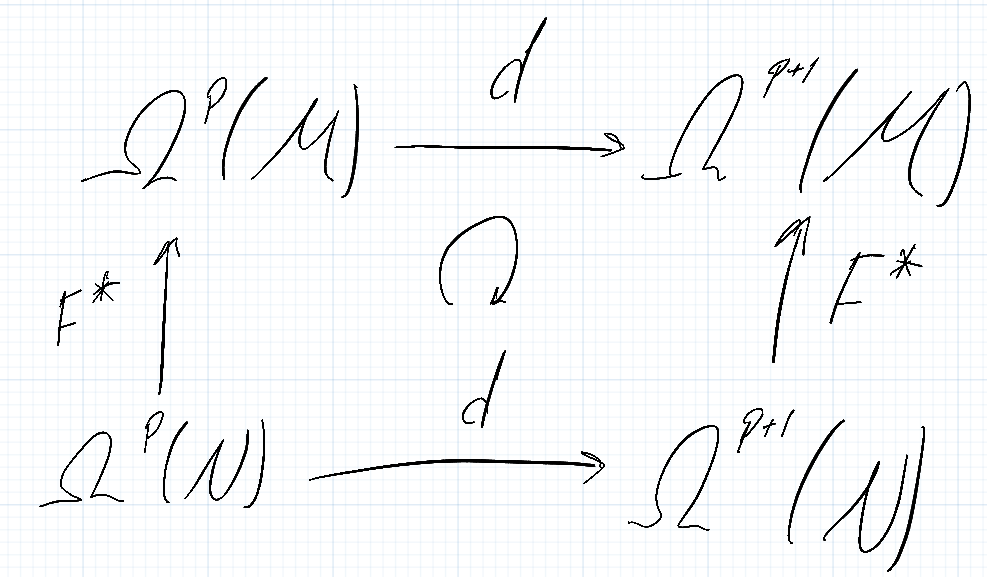
\includegraphics[width=0.55\textwidth]{PullbackCommutesDifferential.png}\end{center}
\end{prop}
\begin{defn}
We say $\omega\in\pformman{p}$ is 
\begin{itemize}
    \item \textbf{closed} if $\dw = 0$
    \item \textbf{exact} if $\exists \omega' \in \pformman{p-1} \st \dw'=w$
\end{itemize}
\end{defn}
$\Note $ Since $\deriv^2 = 0,$ exact implies closed.
\\\\
$\textbf{Important, Interesting and Subtle Question:}$ When does closed imply exact? \\This will motivate a large part of the rest of the course.
\end{section}


\begin{section}{Lecture 3: Towards Integration of Differential Forms on Manifolds}
\begin{subsection}{Building Blocks}
Let $\man$ be an $n$ dimensional manifold. Take $\omega\in\pformman{n}$. Locally, $\omega = f \allthewedge{\dx}{1}{n}$ where $x_i$ are local coords.\\
$\textbf{Goal:}$ Define $\int_\man \omega$ in a coordinate independent way.
\\
First, let $\alphaatlas$ be a smooth atlas for $\man$, where $\chart _\alpha : \chartU_\alpha \to \chart_\alpha(\chartU_\alpha) \subseteq\Real^n$. Let $\trans = \chart_\beta\circ\chart_\alpha^{-1} : \chart_\alpha(\chartU_\alpha\cap \chartU_\beta)\to \chart_\beta(\chartU_\alpha\cap \chartU_\beta)$. We've seen that $\tau_{\alpha\beta}^*\omega(x) = (f\circ \trans)(x) \det(D\trans)\allthewedge{\dx}{1}{n}$.
\\
$\Recall$ Change of variables formula:\\
We say that $D \subseteq\Real^n$ is a domain of integration if its compact and $\partial D$ has measure zero. If $D,E\subseteq\Real^n$ are domains of integration and $F:\bar{D}\to\bar{E}$ is smooth restricting to a diffeomorphism $F : D\to E$, then for $f\in\cts{\bar{E}}$, we have:\\
$$\int_E f \dy_1 ... \dy_n = \int_D (f\circ F) \abs{\det DF} \dx_1 ... \dx_n$$
The  $ \abs{\det DF}$ part is the absolute value of the Jacobian, and is the important part. But our $\trans \omega(x)$ expression didn't have an absolute value part, so we have a discrepancy. Hence the need for the concept of $\textbf{orientation}.$ (Reference for this CoV formula: Strichartz, Way of Anaylsis, Section 15.2).
\begin{defn}

For $\omega \in \pformman{n}$ where $D\subseteq\Real^n$ domain of integration, write $\omega = f \allthewedge{\dy}{1}{n}$ for some $f\in \cts{D}$. Then we define 
$$\int_D \omega \coloneqq \int_D f \allthewedge{\dy}{1}{n} \coloneqq \int_D f \dy_1...\dy_n $$
\end{defn}
The first equals is merely an identity, whilst the second is defining the generalised manifolds definition within this specific situation as the usual multivariable calculus integration we all know and love. This will allow us to extend the manifolds definition out of the puny $D\subseteq\Real^n$ situation to more general domains of integration.

If $U\supseteq D$ is open and we have a diffeomorphism $h: h^{-1}(U)\to U $ (with $h^{-1}(U)\subseteq \Real^n$), then
$$
\int_{h^{-1}(D)} h^* \omega = \int_{h^{-1}(D)} (f\circ h)(x) \abs{\det Dh_x} \allthewedge{\dx}{1}{n} = \int_{h^{-1}(D)} (f\circ h)(x) \abs{\det Dh_x} \dx_1 ...\dx_n 
$$$$
=\begin{cases}
+&\int_D f \dy_1 ... \dy_n \text{  if } \det Dh_x > 0 \\
 - &\int_D f \dy_1 ... \dy_n \text{  if } \det Dh_x < 0
\end{cases}$$
So we can consistently define this, independently of coordinate system, as long as every transition map in our atlas have positive determinant.

\begin{defn}
Let $U\subseteq \Real^n, \omega \in \setform{p}{T^*U}.$ Then the support of $\omega$ is
$$\text{supp } \omega \coloneqq \overline{\{x\in U : \omega(x) \neq 0 \}}$$
We say $\omega$ has compact support if the support of $\omega $ is compact.
\end{defn}
$\Note$ It is a fact that under this assumption of compact support,  we can define $\int_U \omega = \int_D \omega$ where $D$ is any domain of integration containing supp $\omega$. We will not prove this.\\
Thus if $U,V \subseteq \Real^n$ and $\varphi:V \to U$ is a diffeomorphism, provided that $\det \varphi_x > 0 \forall x$, we have $\int_U \omega = \int_V \varphi^* \omega$. So this gives rise to a well-defined integral fro $\omega $ with support contained in a coordinate patch, provided all the transition maps $\trans $ have Jacobians with [XXX adding Jacobian may not be necessary, Dr Jackson didn't. Also I've written $\det D\varphi_x $ where he wrote $\det \varphi_x$. Similarly for the $h$s earlier] positive determinant.
\end{subsection}
\end{section}
\begin{section}{Lecture 4: Orientations, partitions of unity, defining the integral}
\begin{subsection}{Orientations}
\begin{defn}
Let $V$ be a real vector space of dimension $n$, with an order basis $B = (\allthe{b}{1}{n}), B' = (\allthe{b'}{1}{n}).$ We say that $B \myand B'$ have the same $\textbf{orientation}$ if the linear map $T:V\to V : b_i \mapsto b'_i$ has $\det T > 0.$
\end{defn}
So by properties of alternating $n$-forms, $B$ and $B'$ have the same orientation iff for $\omega \in \setform{n}{V^*}$, $ \omega (\allthe{b}{1}{n}) \myand \omega(\allthe{b'}{1}{n})$ have the same sign (follows from proposition in lecture 1).
\begin{defn}
An orientation $\Lambda$ on $V$ is an equivalence class of ordered bases $[B]$, where $B \sim B'$ iff they have the same orientation.
\end{defn}
$\Note$ There are exactly two equivalence classes for any given vector space $V$.
\\\\
If $\varphi : V \to W$ isomorphism of vector spaces, the given an ordered basis $B = (\allthe{b}{1}{n}) $ of V, we can induce an ordered basis $\varphi(B) = (\varphi(b_1),...,\varphi(b_n))$ of $W$. Thus given an orientation $\Lambda$ on $V$,  we have an orientation $\varphi(\Lambda)$ on $W$.
\begin{defn}
We say that $\varphi$ is $\textbf{orientation preserving}$ if $\varphi: V \to W$ is an isomorphism of vectors spaces with orientations $\Lambda_V \myand \Lambda_W$ respectively, such that $\varphi(\Lambda_V) = \Lambda_W$.
\end{defn}
\begin{exmp}
If $V = \Real^n$, then $(\allthe{e}{1}{n})$ defines an orientation on $V$, called the positive orientation.
\end{exmp}\noindent
Now for a manifold $\man$, the idea is to ``consistently'' orient $\tang$ for each $\xman$. 
\begin{exmp}
Consider first, the special case $\man = U \subseteq \Real^n$. There exists a natural isomorphism $D\varphi _ x : \tang \xrightarrow[]{\cong} \Real^n$ (Jacobians of diffeomorphisms give isomorphism of tangent spaces). Let $\triangle_x^+$ be the orientation on $\tang$ induced by $D\varphi_x$ from the positive orientation on $\Real^n$, i.e. $\triangle_x^+$ is the unique orientation such that $D\varphi$ is orientation preserving. So we can consistently orient tangent spaces of subsets of $\Real^n$.
\end{exmp}\noindent
$\textbf{General Case:}$ Let $\alphaatlas$ be an atlas for $\man$, where $\man$ is now any smooth manifold. We orient the charts and then glue together the patches. On each $\chartU_\alpha$, define an orientation: take the unique orientation such that $(D\varphi_\alpha)_x : \tang \to T_{\varphi_\alpha(x)} \varphi_\alpha(\chartU_\alpha) \cong \Real^n$ is orientation preserving. This is called the $\textbf{positive orientation}$ on the coordinate patch $\chartU_\alpha$.
\begin{defn}
We say that $\man$ is $\textbf{orientable}$ if there exists an atlas $\alphaatlas$ and orientations $\Lambda_x^+$ on each $\tang\,\xman$ such that $\forall \alpha,\forall x \in \chartU_\alpha, \, \triangle_x^+$ is the positive orientation on the chart $(\chartU_\alpha,\varphi_\alpha)$.
\end{defn}
\noindent
$\Note$ This is equivalent to the existence of an atlas with $\det D_x(\trans)> 0 \forall \alpha, \beta, \xman$.\\
Back to differential forms: Want to define $\int_{\man} \omega$\\
$\Notation$ $\Omega^p_c(\man) = \{\omega \in \pformman{p} : \omega \text{ has compact support} \}$\\
So in particular, if $\man$ is compact, then $\pformman{p} = \compactpformman{p}$. \\
Let $\omega \in \pformman{n}$, where $\dim \man = n$. Assume supp $\omega \subseteq\chartU$ where $(\chartU,\chart)$ is a chart of $\man$, and $\chart : \chartU \to \chart(\chartU)\subseteq\Real^n$. Assume that $(\chartU,\chart)$ is positively orientated. Consider $\chart^{-1} : \chart(\chartU) \to \chartU$ so that $(\chart^{-1})^* \omega \in \Omega_c^p(\chart(\chartU)))  $ i.e. supp $((\chart^{-1})^*\omega)\subseteq\chart(\chartU).$
\begin{defn}
$\int_\man \omega \coloneqq \int_{\chart(\chartU)} (\chart^{-1})^*\omega$
\end{defn}
Does this depend on $(\chartU,\chart)$? Let $(\chartV,\psi)$ also be a positively oriented chart such that supp$\omega \subseteq \chartV$. We need to show $ \int_{\chart(\chartU)} (\chart^{-1})^*\omega =  \int_{\psi(\chartV)} (\psi^{-1})^*\omega$. Let $\tau \coloneqq \psi \circ \varphi ^{-1} : \chart(\chartU\cap \chartV) \to \psi(\chartU\cap\chartV) \subseteq \Real^n$ be the transition map.
\begin{center}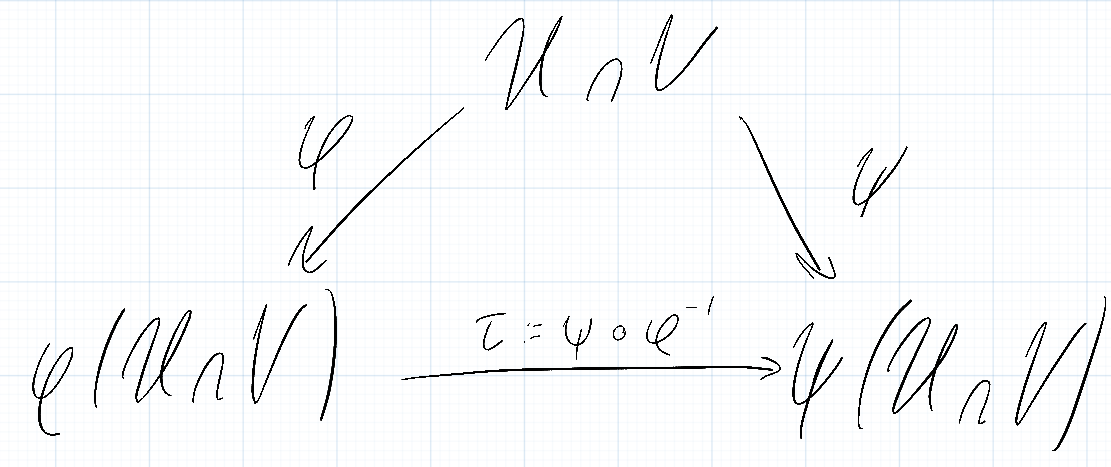
\includegraphics[width=0.55\textwidth]{integrationofcharts.png}\end{center}
$\KeyPoint$ Since both are positively oriented, $\det D\tau > 0$.\\
Hence $\int_{\psi(\chartV)} (\psi^{-1})^*\omega = \int_{\psi(\chartU \cap\chartV)} (\psi^{-1})^*\omega$ because supp $\omega \subseteq\chartU\cap\chartV$\\
$ = \int_{\chart(\chartU \cap\chartV)} \tau^*(\psi^{-1})^*\omega$ because of definition\\
$= \int_{\chart(\chartV\cap\chartU)} (\chart^{-1})^*\psi^*(\psi^{-1})^*\omega$ by composition property of pullbacks\\
$= \int_{\chart(\chartV \cap\chartU)} (\chart^{-1})^*(\psi\circ\psi^{-1})^*\omega$\\
$=\int_{\chart(\chartV \cap\chartU)} (\chart^{-1})^*\omega$. And since $(\chart^{-1})^*\omega =0 $ outside of $\chart(\chartV\cap\chartU)$. Hence the integral is equal to $\int_{\chart(\chartU)}(\chart^{-1})^*\omega.$ So the integral is indeed well-defined.
\end{subsection}
 \begin{subsection}{Partitions of Unity}
 What if supp $\omega$ is not contained within a single coordinate chart? 
 \begin{defn}
 Given an open cover $U = \{U_\alpha\}$ of a manifold $\man$, a $\textbf{partition of unity}$ us a collection of smooth functions $\{f_\alpha\}$, $f_\alpha : \man \to [0,1]$ such that:
 \begin{enumerate}
     \item supp $f_\alpha \subseteq U_\alpha$
     \item $\sumfromto{\alpha}{}f_\alpha(x) = 1 \forall \xman$
     \item $\forall\xman\, \exists U$ open with $x\in U \st $ supp $f_\alpha \cap U$ is nonempty only for finitely many $\alpha$.
 \end{enumerate}
 \end{defn}
  $\Note $ The intuition here is that these are ``a collection of functions that sum everywhere to give you 1''. (3) Ensures that $\sumfromto{\alpha}{}f_\alpha(x)$ is everywhere a finite sum.
  \begin{exmp}
  $\man = S^1 = \{x\in\Real^2 : \abs{x} = 1 \}, U_1 = S^1\backslash\{(1,0)\}, U_2 = S^1\backslash\{(-1,0)\}$. Let $f_1(\cos\theta,\sin\theta) = \frac{1}{2} - \frac{1}{2} \cos \theta, f_1(\cos\theta,\sin\theta) = \frac{1}{2} + \frac{1}{2} \cos \theta$. This is a partition of unity compatible with the open cover $U_1,U_2.$
  \end{exmp}\noindent
  We don't usually engage with these in a hands on way, we're mostly just satisfied that they exist for our purposes.\\
  $\Note$ Given $\man$ manifold, $U = \{U_\alpha\}$ an open cover, there exists a partition of unity compatible with $U$. This a fact we will take as given.
 \end{subsection}
\begin{subsection}{Defining the Integral}
\begin{prop}
$\man$ an $n$ dimensional manifold is orientable iff $\exists \omega \in\pformman{n}$ which is non-vanishing i.e. $\omega(x) \neq 0 \forall \xman$. 
\end{prop}\noindent
Such a non-vanishing top-degree form is called a $\textbf{volume form}$ on $\man$. ``Heuristically, ... infinitesimal unit of volume everywhere on our manifold.''
\begin{proof}
$\Rightarrow:$ Assume $\omega\in\pformman{n}$ is non-vanishing. Given a ordered basis $\allthevs{1}{n}$ of $\tang$, let's call it positively oriented if $\omega(x)(\allthevs{1}{n})>0.$ For all $\xman$ we can thus define an orientation on $\tang$: Take any atlas $\alphaatlas$; then on $\chartU_\alpha$ can write $\omega = g_\alpha \chart^*_\alpha ( \allthewedge{\dx}{1}{n})$ where $x_i$ are coordinates on $\chart(\chartU_\alpha)\subseteq \Real^n.$ Since $\omega \neq 0,$ either $g_\alpha > 0$ or $g_\alpha <0$ for all $x \in \chartU _\alpha$. If the latter, simply exchange $x_1$ and $x_2$ to make $g_\alpha>0 \forall x\in\chartU_\alpha$. This produces an orientation of $\man$.\\
$\Leftarrow$: Let $\man$ be orientable with $\alphaatlas$ atlas with positively oriented charts. Consider $\omega_\alpha = \chart^*_\alpha \allthewedge{\dx}{1}{n}$ on $\chartU_\alpha$, where $x_i$ are coordinates on $\chart(\chartU_\alpha).$ Let $\{f_\alpha\}$ be a partition of unity with respect to $\{\chartU_\alpha\}$ (here interpreted as just a cover of $\man$). Then define $$\Tilde{\omega}_\alpha = f_\alpha \cdot \omega_\alpha \in \Omega^n(\chartU_\alpha)$$ We can extend this by zero (its zero outside the original domain) outside $\chartU_\alpha$ to get $\Tilde{\omega}_\alpha \in \pformman{n}.$ Define $\omega \coloneqq \sumfromto{\alpha}{} \Tilde{\omega}_\alpha\in\pformman{n}$. This is a non-vanishing, which follows easily from the definition of the partition of unity.
\end{proof}\noindent
So far: we've defined $\int_\man \omega$ for $\omega \in \compactpformman{n}$ such that supp $\omega$ is contained in a single coordinate chart, which is an incredibly strong condition to demand. We can now extend this definition.
\begin{defn}
Let $\alphaatlas$ be a positively oriented atlas for $\man$ and left $\{f_\alpha\}$ be a partition of unity with respect to the cover $\{\chartU_\alpha\}$. Then supp $f_\alpha \omega \subset  \chartU_\alpha$, so we can define:
$$\int_\man \omega \coloneqq \sumfromto{\alpha}{} \int_{\chartU_\alpha} f_\alpha \omega$$
\end{defn}
\begin{lemma}
This definition does not depend on the charts $\alphaatlas$ or on the partition of unity $\{f_\alpha\}$.
\end{lemma}
\begin{proof}
We've shown already that if supp $\omega \subset \chartU_\alpha$, then $\int_{\chartU_\alpha} \omega$ does not depend on the chart, provided that it is positively oriented. \\
Let $\varalphaatlas$ be a different atlas, also positively oriented, and let $\{g_\beta\}$ be a different partition of unity, with respect to $\{\chartV_\alpha\}$. Then $\int_\man \omega \coloneqq \sumfromto{\alpha}{} \int_{\chartU_\alpha} f_\alpha \omega = \sumfromto{\alpha,\beta}{} \int_{\man} f_\alpha g_\beta \omega$ because for each $\alpha$ we have $\int_\man f_\alpha \omega = \int_{\chartU_\alpha}f_\alpha \omega$, and $\sumfromto{\beta}{} g_\beta = 1, \,\therefore  \int_{\chartU_\alpha}f_\alpha \omega =  \int_{\chartU_\alpha}f_\alpha (\sumfromto{\beta}{}g_\beta)\omega = \sumfromto{\beta}{}\int_{\chartU_\alpha}f_\alpha g_\beta \omega$, because sum is locally finite in the sense of 3. from definition of partition of unity.\\
In the opposite direction, $\int_\man \omega = \sumfromto{\alpha,\beta}{~}  \int_\man f_\alpha g_\beta \omega = \sumfromto{\beta}{} \int_\man (\sumfromto{\alpha}{}f_\alpha )g_\beta \omega = \sumfromto{\beta}{}\int_\man g_\beta \omega$.
\end{proof}
\begin{prop}
Let $\man$, $\nan$ be orientable manifolds of dimension $n$. Let $\omega, \eta \in \compactpformman{n}$. Then integration on manifolds has the following properties:
\begin{enumerate}
    \item (Linearity) $\int_\man (a \omega + b\eta) = a \int_\man \omega  + b \int_\man \eta$ where $a,b \in \Real$.
    \item (Reversal) Let $\overline{\man}$ be $\man$ with the opposite orientation. Then $\int_{\overline{\man}}\omega=-\int_{\man}\omega.$
    \item (Positivity) Let $\omega$ be a volume form on $\man$ compatible with orientation. Then $\int_\man \omega > 0.$
    \item (Change of Variables) If $F : \nan \to \man $ is a diffeomorphism preserving the orientations, then $\int_\man \omega = \int_\nan F^*\omega$.
\end{enumerate}
\end{prop}
\begin{proof}
1., 2. are exercises.\\
3. Choose $\alphaatlas$ positively oriented atlas. Then on $\chartU_\alpha$, $\omega = g_\alpha \chart ^*_\alpha \allthewedge{\dx}{1}{n}$ for some $g_\alpha > 0$. So $\int_\man \omega = \sumfromto{\alpha}{}\int_{\chartU_\alpha} f_\alpha \omega, $ and each $\int_{\chartU_\alpha} f_\alpha\omega > 0,$ which gives the result.\\
4. If $\alphaatlas$ positively oriented atlas on $\man$, we can define $\chartV_\alpha = F^{-1}\chartU_\alpha$ and $\varchart_\alpha = \chart_\alpha \circ F$ to get an atlas on $\nan.$ Then this atlas is positively oriented because $F$ is orientation preserving. Let $\{f_\alpha\}$ be a partition of unity with respect to $\{\chartU_\alpha\}$. Then $\{f_\alpha \circ F\}$ is a partition of unity with respect to $\{\chartV_\alpha\}$. So we can calculate 
$$\int_\nan F^*\omega = \sumfromto{\alpha}{}\int_\nan (f_\alpha \circ F) F^*\omega = \sumfromto{\alpha}{} \int_\nan F^*(f_\alpha \omega) = \sumfromto{\alpha}{} \int_\man f_\alpha \omega \eqqcolon \int_\man \omega$$ With the equalities coming in order from: using the partition of unity $\{f_\alpha \circ F\}$, definition of pullback, by result for forms with support contained in a single coordinate chart, definition.
\end{proof}
\end{subsection}
\end{section}
\begin{section}{Lecture 5: Manifolds with Boundary}
$\Notation \, \Real_+ ^n = \{(\allthe{x}{1}{n})\in \Real^n : x_n \geq 0\},\, \partial \plusReal \cong \Real ^{n-1} \times \{0\}$\\\\
\begin{defn}
Let $U \subseteq\plusReal$ be open and let $ F : U \to \plusReal$ be a function. We say that $F$ is $\textbf{smooth}$ if it can be extended to some smooth function, i.e. $F : \Tilde{U}\to \Real^m$ where $U \subseteq \Tilde{U}$ and $\Tilde{U}$ is open in $\Real^n,$ where $F : \Tilde{U} \to \Real^m$ is smooth in the usual sense.
\end{defn}
\begin{defn}
A $\textbf{manifold with boundary}$ of dimension $n$ is a second countable Hausdorff topological space $\man$ $\st \exists $ open covering $\{\chartU_\alpha\}$ and for all $\alpha $ homeomorphism $\chart_\alpha : \chartU_\alpha \to \chart_\alpha(\chartU_\alpha) \subseteq \plusReal$ such that each transition map $\trans  = \chart_\beta \circ \chart_\alpha ^{-1}$ is a diffeomorphism.\\
The $\textbf{boundary}$ of $\man$ is $\partial \man \coloneqq \{\xman : \exists \alpha \st \chart_\alpha(x) \in \partial \plusReal\}$
\end{defn}
The $(\chartU_\alpha,\chart_\alpha)$ are called charts, and $\alphaatlas$ is called an atlas. We define a maximal atlas for manifolds with boundary in the same way as for ordinary smooth manifolds.\\
$\Note$ $\partial\man$ is closed in $\man$\\
$\Note$ $\man^\circ \coloneqq \man \backslash \partial \man$ is a manifold of dimension $n$.\\
\begin{exmp}
\begin{enumerate}
    \item $\man = [0,1], \partial \man = \{0,1\}$
    \item $D \coloneqq \{ x\in\Real^n : \abs{x} \leq 1$ has $\partial D = S^{n-1}$
    \item $\man = [0,1] \times S^1$ has $\partial\man \cong S^1\sqcup S^1$
\end{enumerate}
\end{exmp}\noindent
$\Note$ We can define tangent spaces, differential forms for manifolds with boundary in the same way as for the usual smooth manifolds without boundary. The definition of orientation/orientable is the same as usual. \\
$\Note$ If a manifold with boundary $\man$ is orientable, so is $\partial \man$. As a convention, the positive orientation on $\partial\plusReal$ is given by $(-1)^n \allthewedge{\dx}{1}{n-1}.$ This induces positive orientation on $\partial \man$.\\
$\Note$ Partitions of unity for any open cover $\{U_\alpha\}$ on $\man$, a manifold with boundary, are defined in the same way as usual. If $\man$ is orientable, then there is a partition of unity with respect to any open cover. So if $\omega \in \compactpformman{n}$ then we can define $\int_\man \omega$ in the same way as usual.
\end{section}
\begin{section}{Lecture 6: Stokes Theorem}
``Grown up version of Fundamental Theorem of Calculus''\\
\begin{thm}
For $\man$ a manifold with boundary of dimension $n$, and $\omega \in \compactpformman{n-1}$, we have $$\int_{\partial \man} \omega = \int_\man \dw$$
\end{thm}
\begin{proof}
We proceed by special cases:
\\Case 1 : $\man = \plusReal$\\
Since $\omega $ has compact support, $\exists R > > 0 \st $ supp $\omega \subseteq \mathcal{R} \coloneqq [-R,R]^{n-1} \times [0,R]$. Write $\omega = \sumfromto{i=1}{n-1} f_i \dx_1 \wedge ... \wedge \hat{\dx_i} \wedge ... \wedge \dx_n$, where $f_i$ is smooth. Then $$\dw = \sumfromto{i,j = 1}{n} \iparderivof{j}{f_i}\dx_j \wedge \dx_1 \wedge ... \wedge \hat{\dx_i} \wedge ... \wedge \dx_n$$
$$ = \sumfromto{i=1}{n} (-1)^{i-1} \iparderivof{i}{f_i} \allthewedge{\dx}{1}{n}$$
So $\int_\man \dw= \sumfromto{i=1}{n} (-1)^{i-1} \int_0^R \int_{-R}^R ... \int_{-R}^R\iparderivof{i}{f_i} \dx_1 ... \dx_n$. Because everything is smooth, we can do these integrals in any order. Let do $x_i$ first:
\\Then for first $n-1$ terms, via Fundamental Theorem of Calculus:
$$\sumfromto{i=1}{n} (-1)^{i-1} \int_0^R \int_{-R}^R ... \int_{-R}^R[f_i(x)]^{x_i = R}_{x_i = -R}\, \dx_1 ... \hat{\dx_i}... \dx_n = 0$$
This is zero because $\omega = 0$ on the boundary of $\mathcal{R}$. Thus $$\int_\man \dw = (-1)^{n-1} \int_{-R}^R ... \int_{-R}^R \int_0^R \iparderivof{n}{f_n} (x) \dx_n \dx_1... \dx_{n-1} $$
$$= (-1)^{n-1}\int_{-R}^R ... \int_{-R}^R [f_n(x)] ^{x_n = R} _ {x_n=0} \dx_1...\dx_{n-1} \text{ by FTC}$$
$$= (-1)^{n}\int_{-R}^R ... \int_{-R}^R f_n(x_1,...x_{n-1}, 0) \dx_1...\dx_{n-1} \, \text{ because } f(R) = 0 $$
On the other hand, $\int_{\partial \man} \omega = \sumfromto{i}{} \int_{\partial \man \cap \mathcal{R}} f_i(x_1,...,x_{n-1},0) \dx_1 \wedge ... \wedge \hat{\dx_i}\wedge ... \wedge \dx_n$\\
Exercise: Show that $\dx_n \mid _{\partial  \man} = 0$\\
So $\int_{\partial \man} \omega = \int_{\partial \man \cap \mathcal{R}} f_n(x_1,...,x_{n-1},0) \dx_1...\dx_{n-1}$\\
Case 2: $\man = \Real ^n$.\\
Then supp $\omega \subseteq [-R,R]^n$ for some $R>>0$. The same computation shows both sides are zero in this case: 
$$\int_{\partial \man} \omega = \int_\man \dw = 0$$
Case 3: Let $\man$ be an arbitrary oriented manifold with boundary.\\
First suppose supp $\omega \subseteq \chartU _\alpha$ for some chart. Then
$$\int_\man \dw = \int_{\plusReal} (\chart_\alpha^{-1})^* \dw = \int_{\plusReal} d((\chart_{\alpha} ^{-1})^* \omega)$$
And $$ \int_{\plusReal} d ((\chart_\alpha^{-1})^* \omega ) =  \int_{\partial\plusReal} ( \chart_\alpha ^{-1} )^* \omega$$
by the above cases.\\
General case: Use partition of unity.\\
Cover supp $\omega$ by charts $\chartU_\alpha$ and take a partition of unity with respect to this cover, $1 = \sumfromto{\alpha}{} f_\alpha$.\\
Then $$\int_{\partial \man} \omega = \sumfromto{\alpha}{} \int_{\partial \man} f_\alpha \omega = \sumfromto{\alpha}{} \int_\man d(f_\alpha \omega) \text{ by case 3. }$$
 $$ = \sumfromto{\alpha}{} \left( \int_\man \df_\alpha \wedge \omega + \int_\man f_\alpha \dw\right) \text{ by Leibniz property}$$
And this is $\int_\man (\sumfromto{\alpha}{}\df _\alpha)\wedge \omega + \sumfromto{\alpha}{}\int_\man f_\alpha \dw$. First term is $\int_\man \cancelto{0}{d(1)}\wedge \omega = 0$, and second term is $\int_\man (\sumfromto{\alpha}{}f_\alpha) \dw = \int_\man \dw$, proving Stokes' Theorem.
\end{proof}
\end{section}
\begin{section}{Lecture 7: Application of Stokes' Theorem}
Stokes' Theorem implies many of the classical theorems of (multivariate) calculus:
\begin{enumerate}
    \item Fundamental Theorem of Calculus : If $f : [a,b] \to \Real$ smooth, then $\int_a^b f'(x) \dx = f(b) - f(a). $ (Proof: Exercise) 
    \item Green's Theorem (See problem sheet)
    \item Integration by parts
\end{enumerate}
\begin{thm} (Integration by Parts) Let $\man$ be an $n$-dimensional manifold with boundary, and $\omega \in \compactpformman{p}, \eta \in \compactpformman{n-p-1}$ for $p \in \{0,...,n-1\}$. Then
$$\int_{\partial \man} \omega \wedge \eta = \int_{\man} \dw \wedge \eta + (-1)^p \int_\man \omega \wedge \deriv \eta$$
\end{thm}
\begin{proof}
Direct from Stokes' Theorem and Leibniz rule.
\end{proof}
\begin{corollary}{(Integrals of Exact Forms)}
Let $\man$ be an $n$-dimensional manifold without boundary, let $\omega \in \compactpformman{n}$ be exact. Then$\int_\man \omega = 0$
\end{corollary}\noindent
\begin{semiproof}
Follows by rewriting $\omega $ in terms of an $n-1$-form and applying Stokes' Theorem. Since the boundary is empty, the integral will be.
\end{semiproof} 
\begin{corollary}{(Integrals of Closed Forms over Boundaries)} Let $\man$ be an orientable manifold with boundary, of dimension $n$. Let $\omega \in \compactpformman{n-1}$, closed (exterior derivative equals 0). Then $\int_{\partial\man}\omega = 0$.
\end{corollary}\noindent
\begin{semiproof}
$dw = 0 $ so applying Stokes' Theorem immediately gives result.
\end{semiproof}
\begin{defn}
Let $\man$ be orientable manifold of dimension $n$, let $\omega \in \compactpformman{k}$. Let $\nan \subset \man $ be a submanifold of dimension $k$. We define $\omega\restrict{\nan} \coloneqq i^* \omega,$ where $i:\nan\xhookrightarrow{}\man$. Then $\omega\restrict{\nan} \in \compactpformnan{k}.$
\end{defn}

\begin{prop}
Let $\man$ be an orientable manifold of dimension $n$, with submanifold $S\subset \man$. Assume $S$ is compact, orientable and $\partial S = \varnothing$. Let $\omega \in \compactpformman{k}$ be closed, and such that $\int_S \omega \neq 0.$ Then:
\begin{enumerate}
    \item $\omega$ is not exact.
    \item $S$ is not the boundary of any orientable compact manifold $\nan \subset \man$.
\end{enumerate}
\end{prop}\noindent
\begin{proof}
Easy exercise.
\end{proof}
\begin{theorem}
(Brouwer's Fixed Point Theorem) \\
Let $D = \{x\in\Real^n : \abs{x} \leq 1\},\partial D = S^{n-1}.$ Let $f : D \to D $ smooth map. Then $f$ has a fixed point,  i.e. $\exists x \in D \st f(x) = x.$
\end{theorem}
\begin{proof}
Assume not. Then we can define a map $g : D \to \partial D$ as follows: For each $x\in D$, draw a line from $f(x)$ to $x$, and let $g(x)$ be where this line intersects $\partial D$. Since, $f(x) \neq x$ this is well-defined, and it is smooth. Since $S^{n-1} = \partial D$ is orientable, there exists $\omega \in \Omega^{n-1}({\partial D})$ nowhere vanishing (i.e. $\omega$ is a volume form). So $\dw \in \Omega^n (\partial D)$ which is an $n-1$-dimensional manifold, so $\dw = 0.$ Thus:
$$0 < \int_{\partial D} \omega = \int_{\partial D} g^* \omega = \int _D \deriv g^* \omega = \int_D g^*(\cancelto{0}{\dw}) = 0 \,\#$$
(using the fact that integrals of volume forms are positive, $g \restrict{\partial D} = \id$, Stokes' Theorem, and the fact that pullback respects exterior derivative successively). Therefore $f$ does indeed have a fixed point.
\end{proof}
\begin{exmp}
Recall $\deriv ^2 = 0,$ so all exact forms are closed. Let $\man = \Real^2 \backslash \{0\}, $ and let 
$$\omega = \frac{x}{x^2+y^2} \dy - \frac{y}{x^2+y^2} \dx \in \pformman{1}$$
This is closed:
$$\dw = \left(\frac{\partial}{\partial x} \left(\frac{x}{x^2+y^2}\right) + \frac{\partial}{\partial y}\left( \frac{y}{x^2+y^2}\right)\right) \dx \wedge \dy = 0$$
$\Claim$This is not exact. Suppose $\exists f \in \cts{\man} \st \df = \omega. $ Then in particular, this is true on $S^1 \subset \man.$
Let $\gamma : [0,2\pi] \to S^1, \theta \mapsto (\cos\theta,\sin\theta).$ Then $\int_{S^1} \omega = \int_0^{2\pi} \gamma^* \omega = ... = \int_0 ^{2\pi} \deriv \theta = 2\pi.$\\
But $\int_{S^1} = \int_{\partial S^1} f = 0 \#$ (using Stokes' and $\partial S^1 = \varnothing$)
\end{exmp}
So the fact that $\omega$ does not extend smoothly to the origin is significant, its not closed-but-not-exact-ness is telling us that there is a hole in our manifold, hinting at the beginnings of de Rham cohomology.
\begin{defn}
Let $f : \man \to \nan,$ $g:\man \to \nan$ be smooth maps of manifolds. We say that $f$ and $g$ are $\textbf{smoothly homotopic}$ is there exists a smooth homotopy between then, i.e. a smooth function 
$$H: [0,1] \times \man \to \nan \st H\restrict{\{0\} \times \man} = f \myand H\restrict{\{1\} \times\man} = g$$
\end{defn}
$\Note$ This is an equivalence relations on smooth maps $\man \to \nan$; we write $f \sim g$ iff $f$ and $g$ are smoothly homotopic.
\begin{prop}
Let $f,g : \man \to \nan$ be smooth maps of manifolds, and assume $f\sim g$. If $\omega \in \compactpformnan{n}$ is closed, then $\int_\man f ^* \omega = \int_\man g^* \omega$.
\end{prop}
\begin{proof}
Consider the $n+1$-dimensional manifold, $[0,10\times \man$. Then 
$$\int_{\partial ([0,1]\times \man)} H^*\omega = \int_{[0,1]\times \man} \deriv ( H^* \omega) = \int_{[0,1]\times\man} H^*\dw = 0$$
using Stokes' and the fact $\omega$ is closed, successively. On the other hand,
$$\int_{\partial ([0,1]\times \man)} H^* \omega = \int_{\{1\}\times \man} H^*\omega - \int_{\{0\}\times \man} H^*\omega = \int_\man g^*\omega - \int_\man f^* \omega$$
because $H$ is a homotopy from $f$ to $g$.
\end{proof}
\begin{theorem}
(Fundamental Theorem of Algebra) Every polynomial $p(z) = z^n + a_{n-1}z^{n-1} + ... + a_1 z + a_0$ has a root in $\mathbb{C}$ for $n \geq 1.$
\end{theorem}
\begin{proof}
Assume not, so $p: \mathbb{C} \to \mathbb{C}\backslash \{0\}.\, \exists R > > 0 \st$where $\abs{z} \geq R,$ we have $\abs{\frac{p(z)-z^n}{z^n}}\leq \frac{1}{2},$ since $\frac{p(z) - z^n}{z^n} \to 0$ as $z\to \infty.$ Identify $\Real^2 \cong \mathbb{C}$. Write $D_R = \{z\in \Real^2 : \abs{z} \leq R\},\, \partial D_R = \{z\in \Real^2 : \abs{z} = R\}\cong S^1$. Define a homotopy $H : [0,1] \times D_R \to \mathbb{C}\backslash\{0\}$ from $p(z)$ to $g(z) = z^n,$ by $H(t,z) = tg(z) + (1-t)p(z).$ Then $\abs{H(t,z)} = \abs{z^n +(1-t)(a_{n-1}z^{n-1} +...+a_0)}\geq \abs{z^n} -(1-t)\abs{a_{n-1}z^{n-1} + ... + a_0} \geq \abs{z^n}(1-\frac{1}{2}) = R^2 \cdot \frac{1}{2},$ so $H(t,z) \neq 0$ and so it is indeed a homotopy\\
Now recall: $\omega = \frac{-y \dx +x dy}{x^2+y^2}$ is closed on $\Real^n\backslash \{0\} \cong \mathbb{C}\backslash \{0\}.$ Writing $g(z)$ as $(r\cos\theta,r\sin\theta) \mapsto r^n (\cos n\theta,\sin n \theta),$ we see $\int_{\partial D_R} g^* \omega = \int_{\partial D_R} p^* \omega = \int_{D_R} p^*(\dw) = 0$ [homotopic and $\omega$ closed, Stokes' and $\omega$ closed successively]. But we can directly calculate $\int_{\partial D_R} g^*\omega = 2\pi n \#$. A contradiction, and so $p(z)$ does indeed have a root.
\end{proof}
\end{section}
\begin{section}{Lecture 8: De Rham Cohomology}
\begin{defn}
Let $\man$ be a smooth manifold of dimension $n$, and let $p\geq 0$. The $\textbf{de Rham complex}$ is the sequence of real vector spaces 
$$0 \xrightarrow[]{\deriv} \cts{\man} \xrightarrow[]{\deriv} \pformman{1} \xrightarrow[]{\deriv} \pformman{2} \xrightarrow[]{\deriv} ...  \xrightarrow[]{\deriv} \pformman{n}  \xrightarrow[]{\deriv} 0$$
\end{defn}
\begin{defn}
We say that $\omega_1,\omega_2 \in \pformman{p}$ are $\textbf{cohomologous}$ if $\omega_1 -\omega_2 = \deriv\eta$ where $\eta \in \pformman{p-1}$.
\end{defn}
\noindent
In particular, $\omega$ is cohomologous to 0 iff $\omega$ is exact.\\
$\Notation$\begin{itemize}
    \item $Z^p(\man) \coloneqq \Ker(\deriv : \pformman{p} \to \pformman{p+1} ) = \{\text{closed } p \text{-forms}\} \subset \pformman{p}$
    \item $B^p(\man) \coloneqq \Ima(\deriv : \pformman{p-1} \to \pformman{p} ) = \{\text{exact } p \text{-forms}\} \subset \pformman{p}$
\end{itemize} 
$\Recall$ $\deriv^2 = 0$, so we have $B^p(\man) \subset Z^p(\man)$ for all $p\geq 0$.\\
$\Note$ $\omega_1, \omega_2 \in Z^p(\man)$ then $\omega_1-\omega_2 \in B^p(\man) \iff $ $\omega_1 \,\&\,\omega_2$ cohomologous.
\begin{defn}
The $p^{th}$ $\textbf{de Rham cohomology group}$ of $\man$ is 
$$H^p(\man) \coloneqq Z^p(\man)/B^p(\man) = \{ [\omega ] : \omega \in Z^p(\man)\}, \,\,p\geq 0$$
where $[\omega]$ is the equivalence class of all $p$-forms cohomologous to $\omega$.
\end{defn}\noindent
$\Note$ $H^p(\man)$ is a real vector space (maybe infinite dimensional (turns out its not most of the time, which is kind of a miracle if you consider even the $p=0$ case)).
\begin{defn}
The $p^{th}$ $\textbf{Betti number}$ of $\man$ is 
$$b_p(\man)\coloneqq \dim_\Real H^p(\man) \in \mathbb{Z}_{\geq 0} \cup \{\infty \}$$
\end{defn}
\begin{prop}
If $\man$ is connected then $H^0(\man) \cong \Real$, i.e. $b_0(\man) = 1.$ Moreover, in general $b_0(\man)  $ is the number of connected components of $\man$.
\end{prop}
\begin{proof}
Assume $\man$ connected. Then $B^0(\man) = 0$, because there are no $-1$-forms. Therefore $\cohomman{0} \cong \coZman{0} = \{f\in \pformman{0} \text{ closed}\} = \{f\in\cts{\man} : \text{locally, } \forall x\in \man, \iparderiv{i}{} f(x) = 0\} = \{f\in\cts{\man} : \text{locally constant i.e. } \forall x \in \man \exists U\subset \man \st x \in U \myand f\restrict{U} \text{ is constant}\} = \Real.$\\
This generalises because the the space of locally constant functions has the rank of the number of connected components; if $\man$ is made up of connected components $C_i$ and $x\in C_1$, then $f\restrict{C_1}$ is constant but there are still $\Real$ many choices for $f\restrict{C_2}$, $\Real$ many for $f\restrict{C_3} ...$ etc. So rank $\coZman{0}$ = number of connected components.
\end{proof}
\begin{exmp}
$\man = S^1$ then $\cohomman{0} \cong \Real$
\end{exmp}
\begin{prop}
$\cohomman{p} = 0 \forall p > n \eqqcolon \dim \man$
\end{prop}
\begin{proof}
Recall that $\pformman{p} = 0 \forall p > n.$ Result immediate.
\end{proof}
\begin{prop}
Let $\man$ be a compact and orientable manifold without boundary, of dimension $n$. Then $\cohomman{n} \neq 0$.
\end{prop}
\begin{proof}
$\man$ orientable so $\exists $ volume form $\omega \in \pformman{n} = \compactpformman{n}$ ($\man$ compact). Then $\omega$ is closed, as $\dw \in \pformman{n+1} = 0$, so $\omega \in \coZman{n}$. We claim $[\omega] \neq 0$, i.e. $\omega$ not cohomologous to zero, i.e. not exact. \\Assume otherwise, $[\omega] = 0$. Then $\omega = \deriv \eta$ where $\eta \in \pformman{n-1},$ so
$$0< \int_\man \omega = \int_\man \deriv \eta = \int_{\partial \man} \eta = 0\,\#$$
\end{proof}
\begin{subsection}{Functoriality of de Rham Cohomology}
\begin{prop}

If $F: \man \to \nan $ is a smooth map of smooth manifolds, then $F^*: \pformnan{p} \to \pformman{p}$ gives rise to vector space maps, $F^*: \cohomnan{p} \to \cohomman{p}$ for $p\geq 0.$
\end{prop}

\begin{proof}
We must show that $F^*:\pformnan{p} \to \pformman{p}$ takes closed forms to closed forms and exact forms to exact forms. By a previous proposition, the diagram below commutes:%commutative diagram
$$\begin{tikzcd}
\centering{}
{\pformnan{p}}\arrow[r,"d"]\arrow[dr,phantom,"\circlearrowright"] \arrow[d,"F^*"] & {\pformman{p+1}} \arrow[d,"F^*"] \\
{\pformman{p}} \arrow[r,"d"]           & {\pformnan{p+1}}  
\end{tikzcd}$$
Therefore if $\omega \in Z^p(\nan) \subset \pformnan{p}$ then $\dw = 0.$ And $F^*\dw = d(F^*\omega) = 0$, so $F^*\omega \in \coZman{p}.$ 
\\Similarly if $\omega \in B^p(\nan)$ with $\deriv \eta = \omega,$ then $F^*\omega = F^*(\deriv \eta) = \deriv(F^*\eta)$ so $F^*\omega \in B^p(\man).$
\end{proof}
\begin{corollary}
If $\man$ and $\nan$ are diffeomorphic manifolds, then $\cohomman{p} \cong \cohomnan{p}$ for all $p \geq 0.$
\end{corollary}
\begin{proof}
Let $F:\man \to \nan$ be a diffeomorphism. Then we claim that $F^*: \cohomnan{p} \to \cohomman{p}$ is an isomorphism of groups. Indeed the map $F^{-1} : \nan \to \man$ is smooth, and $F\circ F^{-1} = \id_\nan$. It follows that $(F^{-1})^*\circ F^* : \cohomnan{p} \to \cohomnan{p}$ is the identity, so $F^*: \cohomnan{p} \to \cohomman{p} $ has an inverse, so it is an isomorphism.
\end{proof}
\end{subsection}
\end{section}
\begin{section}{Lecture 9: Homotopy Invariance of de Rham Cohomology}
Goal is to prove the following theorem:
\begin{theorem}[Homotopy Invariance of de Rham Cohomology]\label{theorem:homotopyinvariance}
 Let $\man$ and $\nan$ be manifolds, with $f,g: \man \to \nan$ that are smoothly homotopic. Then the maps 
$$f^*:\cohomnan{p} \to \cohomman{p}, \,g^*:\cohomnan{p} \to \cohomman{p}$$
are equal.
\end{theorem}
This will be enormously helpful in computing de Rham cohomology groups.\\
If we have $f,g:\man \to \nan$, how can we show that $f^* = g^*$ on cohomology? Well $f^* =g^*$ means that $\forall \omega \in \coZnan{p}$ that $[f^*\omega] = [g^*\omega]$ i.e. $f^*\omega$ is homologous to $g^*\omega$ i.e. $\exists \eta \in \pformman{p-1}$ such that $f^*\omega - g^* \omega = \deriv \eta$.
\begin{defn}
\label{defn:homotopyoperator}
A $\textbf{homotopy operator}$ (or cochain homotopy) from $f^*$ to $g^*$ is a linear map $h:\pformnan{p} \to \pformman{p-1}$ such that $\forall \omega \in \pformnan{p}$ we have \begin{equation}
    f^*\omega - g^*\omega = h(\dw)-\deriv(h(\omega))\tag{$*$}
\end{equation}
\end{defn}\noindent
$\Note$ If $\omega \in \coZnan{p}$ then we get $f^*\omega - g^*\omega = \deriv(h(\omega))$
So if there exists a homotopy operator from $f^*$ to $g^*$ then they give the same map on cohomology groups.
\begin{proof}{of Theorem \ref{theorem:homotopyinvariance}}\\
Let $H:[0,1]\times \man \to \nan $ be a smooth homotopy from $f$ to  $g$.\\
$\textbf{First Claim:}$ Define $i_0 :\man \to \inter \times \man: x \mapsto (0,x)$, and $i_1 :\man \to \inter \times \man: x \mapsto (1,x)$. We claim that if $i_0^* = i_1^*$ on cohomology then $f^* = g^*$ on cohomology.\\
\begin{subproof}
First observe that $H\circ i_0 = f, H\circ i_1 = g$. Now take $\eta \in \pformnan{p}$. We want to show $[f^*\eta ] = [g^*\eta]$. Let $\omega = H^* \eta \in \Omega^p(\inter \times \man). $ Then $f^*[\eta] = [f^*\eta] = [(H\circ i_0)^*\eta] = [i_0^* \circ H^* \eta ] = [i_0^* \omega] = [i_1^*\omega ]$ (by assumption). And $[i^*_1\omega] = [(H\circ i_1)^* \eta] = [g^*\eta] =g^*[\eta]$
\end{subproof}\\
So by the first claim, it suffices to exhibit a homotopy operator from $i^*_0$ to $i_1^*$. Let's define one, namely $$h:\Omega^p(\inter\times\man) \to \pformman{p-1}: \omega(x)(v_1,...,v_{p-1}) \mapsto \int_0^1 \omega(x,t) \left(\frac{\partial}{\partial t}, v_1,...,v_{p-1}\right)$$ with $x\in \man, \allthevs{1}{p-1}\in T_x \man$ and $t$ being the standard coordinate on $\inter$. First observe that $h$ is linear (Check!). We claim $h$ satisfies equation $(*)$ from Definition $\ref{defn:homotopyoperator}$. Since we can check $(*)$ pointwise, we can work locally in coordinates: $$\omega = \sumfromto{\abs{I} = p}{} \omega _I + \sumfromto{\abs{J} = p-1}{} \omega _J,\, \omega_I = g_I \allthewedge{\dx}{i_1}{i_p}, \, \omega_J = \allthewedge{\dx}{j_1}{j_{p-1}}\wedge \dt$$
All terms appearing in $(*)$ are linear over $\Real$, so we can check $(*)$ on each term in this expression for $\omega$.\\
$\omega _I$ case: $\omega_I(x,t)\left(\parderiv{t} , v_1,...,v_{p-1}\right) = 0$ because $\omega_I$ has no $\dt$. So $h(\omega)(\allthevs{1}{p-1})=0\,\,\forall \allthevs{1}{p-1}\in \tang, \forall \xman$ so $\deriv h(\omega) = 0$. And $$h(\dw_I) = h\left(\frac{\partial g_I}{\partial t} \dt \wedge \allthewedge{\dx}{i_1}{i_p} + \sumfromto{j=1}{n}\frac{\partial g_I}{\partial x_j}\dx_j \wedge \allthewedge{\dx}{i_1}{i_p}\right)$$
$$= h\left(\frac{\partial g_I}{\partial t} \dt \wedge \allthewedge{\dx}{i_1}{i_p}\right) + \sumfromto{j=1}{n} h\left( \frac{\partial g_I}{\partial x_j}\dx_j \wedge \allthewedge{\dx}{i_1}{i_p}\right)$$
$$ = \left(\int_0^1\frac{\partial g_I}{\partial t}\dt \right)\wedge \allthewedge{\dx}{i_1}{i_p} + 0$$
(The second term is 0 is because there is no $t$ variable, same logic as why $\deriv h(\omega) = 0$)
$$= \left(g(x,1)-g(x,0)\right)\allthewedge{\dx}{i_1}{i_p}$$
And $i_0^*\omega_I = g(x,0)\allthewedge{\dx}{i_1}{i_p},\, i_1^*\omega_I = g(x,1)\allthewedge{\dx}{i_1}{i_p}$, so we have $(*)$ for things of the form $\omega_I$:
$$\cancelto{0}{\deriv(h(\omega_I))} + h(\dw_I) = i_1^* \omega_I - i_2^*\omega_I$$
$\omega_J$ case: $\omega _J = g_J \allthewedge{\dx}{j_1}{j_{p-1}} \wedge \dt$, where $g_J = g_J(x,t)$.
$$h(\omega) (\allthevs{1}{p-1}) = \int_0^1 \omega_J(x,t) \left(\parderiv{t},\allthevs{1}{p-1}\right) \dt$$
$$ = \int_0^1 \left(g_J(x,t) \allthewedge{\dx}{i_1}{p-1}\wedge \dt \left(\parderiv{t} , \allthevs{1}{p-1}\right)\right)\dt$$
$$= (-1)^{p-1}\int_0^1 \left(g_J(x,t) \dt \wedge \allthewedge{\dx}{i_1}{i_{p-1}}\left(\parderiv{t},\allthevs{1}{p-1}\right)\right)\dt$$
$$= (-1)^{p-1}\int_0^1 \left(g_J(x,t) \allthewedge{\dx}{i_1}{i_{p-1}}\left(\allthevs{1}{p-1}\right)\right)\dt$$
``feeding the $\parderiv{t} $ into the $\dt$''
$$= (-1)^{p-1}\left(\int_0^1 g_J(x,t)\dt\right) \allthewedge{\dx}{i_1}{i_{p-1}}\left(\allthevs{1}{p-1}\right)$$
So $$\deriv(h(\omega)) = \sumfromto{j=1}{n} (-1)^{p-1} \parderiv{x_j} \left(\int_0^1 g_J(x,t)\dt\right)\dx_j \wedge \allthewedge{\dx}{i_1}{i_{p-1}}$$
$$\deriv (h(\omega))= (-1)^{p-1} \sumfromto{j=1}{n} \left(\int_0^1 \frac{\partial g_J}{\partial x_j}(x,t)\dt\right)\dx_j \wedge \allthewedge{\dx}{i_1}{i_{p-1}}$$
And 
$$\dw _J = \deriv( g_J(x,t) \allthewedge{\dx}{i_1}{i_{p-1}}\wedge \dt)$$
$$ = \sumfromto{j=1}{n} \frac{\partial g_J}{\partial x_j} \dx_j \wedge \allthewedge{\dx}{i_1}{i_{p-1}} \wedge \dt + \cancelto{0}{\frac{\partial g_J}{\partial t} \dt \wedge \allthewedge{\dx}{i_1}{i_{p-1}}\wedge \dt}$$
$$h(\dw_J)(\allthevs{1}{p-1}) = \sumfromto{j=1}{n} \left(\int_0^1 \frac{\partial g_J}{\partial x_j} \dt\right)\dx_j \wedge \allthewedge{\dx}{i_1}{i_{p-1}}\wedge\dt\left(\parderiv{t},\allthevs{1}{p-1}\right)$$
$$= (-1)^{p} \sumfromto{j=1}{n} \left(\int_0^1 \frac{\partial g_J}{\partial x_j} \dt\right)\dt \wedge\dx_j \wedge \allthewedge{\dx}{i_1}{i_{p-1}}\left(\parderiv{t},\allthevs{1}{p-1}\right)$$
$$= (-1)^{p} \sumfromto{j=1}{n} \left(\int_0^1 \frac{\partial g_J}{\partial x_j} \dt\right) \dx_j \wedge \allthewedge{\dx}{i_1}{i_{p-1}}\left(\allthevs{1}{p-1}\right)$$
The only difference between these two expressions in (-1) i.e. $h(\dw_J) = -\deriv(h(\omega_J))$. For $\omega_J$, both $i_0^*$ and $i_1^*$ give zero, i.e. $i^*_0\omega_J$ restricts to $\{0\}\times\man$ and $i^*_1\omega_J$ restricts to $\{1\}\times\man$, because $\dt$ vanishes on slices $\{t\}\times \man$. Hence,
$$h(\dw_J) + \deriv (h(\omega_J)) = 0 = i_0^*\omega_J = i_1^*\omega_J$$
So $(*)$ hold for terms of the form $\omega _J$. Therefore $(*)$ holds for terms of the original $\omega$, and so we conclude that $h$ is a homotopy operator from $i_0^*$ to $i_1^*$, and hence $f^*=g^*$ by the first claim, concluding the proof.
\end{proof}
\end{section}
\begin{section}{Lecture 10: Using Homotopy Invariance}
$\Recall$ $f,g:\man\to\nan$ maps of manifolds are called smoothly homotopic if $\exists $ (smooth) $H:\inter \times \man \to \nan \st H\restrict{\{0\}\times \man} = f , \, H\restrict{\{1\}\times \man} = g$
\begin{theorem}[Thm 9.28 of Intro to Smooth Manifolds]
If $f$ and $g$ are homotopic then they are smoothly homotopic i.e. $\exists $ continuous homotopy then $\exists $ smooth homotopy.
\end{theorem}\noindent
Last time we saw Thm \ref{theorem:homotopyinvariance}: $f\sim g \implies f^* = g^*$ on de Rham cohomology\footnote{Surprising: All these differential forms that we defined from the smooth structure on our space end up giving (as we'll see) topological invariants, independent of the smooth structure. We can define many smooth structures on the same manifold that makes them non-diffeomorphic as smooth manifolds, despite being homeomorphic as topological manifolds but the de Rham cohomology will look the same anyway.}. Today we see applications of this.
\begin{defn}
We say $\man$ and $\nan$ are $\textbf{homotopy equivalent}$ if $\exists f:\man \to \nan, \, g: \nan\to\man \st f\circ g \sim \id_\nan , \, g\circ f \sim \id_\man$.
\end{defn}
This is a kind of weakening of the idea of homeomorphism.
\begin{exmp}
\begin{enumerate}[(i)]
    \item $\man = \Real ^n, \, \nan = \{0\}.$ Let $f:\Real^n \to \{0\}$ and $g:\{0\} \xhookrightarrow{} \Real^n$. Then $f\circ g = \id_{\{0\}}$ and $g\circ f : \Real^n \to \Real^n : x \mapsto 0$. Define $H: \inter \times \Real^n \to \Real ^n : (t,x) \mapsto tx$. Thus $H\restrict{\{0\}\times \Real^n} = g\circ f , H\restrict{\{1\}\times \Real^n} = \id_{\Real^n}$. So $\Real^n$ is homotopy equivalent to a point (as is any star-shaped set).
    \item $\man = \Real^2\backslash \{0\}, \nan = S^1 \subset \Real^2$. Let $f: \man \to \nan: x\mapsto \frac{x}{\abs{x}}$ and let $g: \nan \hookrightarrow \man$ be the inclusion. Then $f\circ g = \id_{\nan}, g\circ f \sim \id_{\Real^2\backslash\{0\}}$ via $H(t,x) = tx + (1-t) \frac{x}{\abs{x}}$.
\end{enumerate}
\end{exmp}
\begin{defn}
We say that $U\subseteq \Real^n$ is $\textbf{star-shaped}$ if $\exists x_0 \in U \st \forall x\in U $, the line segment from $x_0$ to $x$ is contained in $U$.
\end{defn}
\begin{prop}\label{prop:homotopyequivalenceimpliescohomologyequivalence}
If $\man $ is homotopy equivalent to $\nan$, then we have isomorphisms $\cohomman{p} \cong \cohomnan{p}, \, p\geq 0$
\end{prop}
\begin{proof}
Let $f: \man \to \nan, \, g:\nan\to \man $ be s.t. $f\circ g \sim \id _{\nan}, \, g\circ f \sim \id_{\man}$. Then $(f\circ g)^* = \id_\nan^*$ i.e. identity map $\cohomnan{p} \to \cohomnan{p},$ and $(g\circ f)^* = \id_\man^*$ similar thing, both by the result from last time. So $f^* = (g^*)^{-1}, g^* = (f^*)^{-1}$ so both are isomorphisms.
\end{proof}
\begin{defn}
We say that $\man$ is $\textbf{contractible}$ if $\man$ is homotopy equivalent to a point.
\end{defn}\noindent
In particular, any star-shaped $U \subseteq \Real^n$ is contractible.
\begin{theorem}[Poincaré Lemma]
If $\man$ is contractible, then $\cohomman{p} = 0 $ for $p\geq 1$.
\end{theorem}
\begin{proof}
By proposition \ref{prop:homotopyequivalenceimpliescohomologyequivalence}, $\cohomman{p} \cong H^p(\{{pt}\})$, and since $\{pt\}$ is zero-dimensional manifold, we know $H^p(\{pt\}) = 0$ for $p\geq 1$ as de Rham cohomology groups vanish for degree higher than dimension of the manifold.
\end{proof}
\begin{prop}[``Being exact is not a local property'']
Let $\man$ be any manifold and take $\omega \in \pformman{k}$ closed for $k> 0$. Then $\forall \xman \exists U \subseteq\man $, a nbd of $x \st \omega\restrict{U}$ is exact. 
\end{prop}
\begin{proof}
WLOG assume $\man \subseteq \Real^n$ (take a small enough nbd of $x$ such that it is contained within a single coordinate chart, then identify $\man$ with its image into this coordinate chart) and $U$ is in a coordinate chart. Take a ball around $x$, $B(x,r)$ where $0<r<<1 \st B(x,r) \subseteq \man.$ Then $B(x,r)$ is contractible, so in particular all closed forms are exact for $k>0$. So $\exists \eta \in \Omega^{k-1}(B(x,r)) \st \deta =\omega\restrict{B(x,r)}$.
\end{proof}\noindent
$\KeyPoint$ Thus de Rham cohomology measures our inability to `lift' these $\eta\restrict{U}$s to all of $\man$.\\
So $\cohomman{0}$ tells us how many connected components $\man$ has. What about $\cohomman{1}$?
\begin{defn}
A $\textbf{path}$ is a smooth map $\gamma : \inter \to \man.$ If $\gamma(0) = a, \gamma(1) = b,$ then we say $\gamma $ is a path from $a$ to $b$. 
\\An (endpoint-preserving) $\textbf{homotopy of paths}$ (from $\gamma_0$ to $\gamma_1)$ is a smooth map $H:\inter\times\inter \to \man \st$$$
H\restrict{\{0\}\times\inter} = \gamma_0, H\restrict{\{1\}\times\inter} = \gamma_1\,, \myand \,H(t,0) = a, H(t,1) = b \,\forall t \in \inter$$
We say $\gamma_0$ and $\gamma_1$ are homotopic.
\end{defn}
$\Recall$ $F,G:\man \to \nan$ are homotopic maps of manifolds (without boundary), then for any $\omega\in\pformnan{k}$ closed, we have $\int_\man F^*\omega = \int_\man G^*\omega$. We now strengthen this result.
\begin{prop}\label{prop:integralofhomotopicpathsequal}
If $\gamma_0,\gamma_1$ are homotopic paths in $\man $ and $\omega \in\pformman{1}$ closed. Then  $\int_{\gamma_{0}}\omega = \int_{\gamma_1} \omega$ (where $\int_{\gamma_0} \omega \coloneqq \int_0^1 \gamma_0^* \omega$).
\end{prop}\noindent
\begin{semiproof}
Let $\gamma_1^{-1}* \gamma_0$ be the path ``$\gamma_0$, then $\gamma_1$ backwards'', i.e.
$$s\in\inter, \, \gamma_1^{-1}* \gamma_0(s) \coloneqq \begin{cases} \gamma_0(2s) &,s\in\left[0,\frac{1}{2}\right] \\ \gamma_1(-2s+2) &,s\in \left[\frac{1}{2},1\right]\end{cases}$$
Let $H:\inter\times\inter \to \man$ be a homotopy from $\gamma_0$ to $\gamma_1$. Then by ``Stokes' Theorem for manifolds with corners'' (which we will not prove):
$$\cancelto{0}{\int_{\inter^2} \deriv(H^*\omega))} = \int_{\partial \inter^2} H^*\omega$$
The cancelling to 0 is because $\omega$ is closed.
% https://tikzcd.yichuanshen.de/#N4Igdg9gJgpgziAXAbVABwnAlgFyxMJZABgBpiBdUkANwEMAbAVxiRAAoyBGAShAF9S6TLnyEUXclVqMWbdpN4ChIDNjwEi3afWatEHMsT6Dh6sUUU7Z+jpOMDpMKAHN4RUADMAThAC2SGQgOBBIkjJ6bAA6UTgwAB44wADGBHA4AHT8yl6+AYjhIUgAzNS6cgYxLnR+fnQA+lw5ID7+SABM1EWIQeW2VTV19cTNrfmlwaGInREVIDFxiSlpmdn8FPxAA
And $\partial \inter^2$ is $$\begin{tikzcd}
{(0,1)} \arrow[r, "\text{const.}"] & {(1,1)} \arrow[d, "\gamma_1"]      \\
{(0,0)} \arrow[u, "\gamma_0"]      & {(1,0)} \arrow[l, "\text{const.}"]
\end{tikzcd}$$ so $\int_{\partial\inter^2} H^*\omega = \int_{\gamma_0}\omega + 0 - \int_{\gamma_1} \omega +0$, giving the result.
\end{semiproof}
\begin{defn}
We say $\man$ is $\textbf{simply connected}$ if any parth from $x$ to $x$ is homotopic to a constant path (i.e. to point) for some (or equivalently any) $\xman$.
\end{defn}
$\Note$ This is equivalent to \begin{enumerate}
    \item Every map $S^1 \to \man$ is homotopic to the constant map
    \item $\pi_1(\man) = \{e\}$, i.e. the fundamental group is trivial.
\end{enumerate}
\begin{prop}
If $\man$ is simply connected, then $\cohomman{1} = 0$.
\end{prop}
\begin{proof}
We claim that a closed 1-form is exact iff $\int_\gamma \omega = 0$ for all loops (i.e. paths from $x$ to $x$) $\gamma$.\\
    \begin{subproof}
    $\impliesdirection$ Let $\omega \in \pformman{1}$ be exact. Then it is closed, so by proposition \ref{prop:integralofhomotopicpathsequal} we have $\int_\gamma \omega =  \int_{\text{constant loop}}\omega = 0$, because $\man $ is simply connected.\\
    $\impliedbydirection$ Now supposed $\int_\gamma \omega =0$ for all loops $\gamma$. Fix some $x_0\in \man$ and define $f(x) \coloneqq \int_p \omega$ where $p$ is any path from $x_0$ to $x$. This is well-defined: If $p'$ is a different path, then consider $\gamma = p' * p^{-1}$, which is homotopic to a constant because $\man$ is simply connected. Then $ 0 = \int_\gamma \omega = \int_p \omega - \int_{p'} \omega.$ Hence $\int_p \omega = \int_{p'}$ so is indeed well-defined.\\
    And $\df = \omega :$ check this locally on a coord patch in $\Real^n$ and use Fundamental Theorem of Calculus.
    \end{subproof}
    To finish the proof of the proposition, note that for any closed $\omega\in\pformman{1}, \int_\gamma \omega = 0$ for any loop $\gamma$ since $\gamma$ homotopic to a constant because $\man$ is simply connected. Hence $\omega$ is exact, and so $\cohomman{1} = 0$.
\end{proof}\noindent
$\Note$ In order for this to be a strictly topological statement, you'll have to take my word for it that any continuous path is homotopic to a smooth path, see Intro to Smooth Manifolds.\\
$\Note$ (For those who know about $\pi_1)$ In fact more is true: there is a well-defined map $$\cohomman{1} \to \Hom{\pi_1(\man)}{\Real} : [\omega] \mapsto \left( [\gamma] \mapsto \int_{\gamma'} \omega\right)$$with $\gamma'$ being a smooth representative of $\gamma$'s homotopy class, which we assert exists. This map is an isomorphism. See Intro to Smooth Manifolds 17.17.
\end{section}


\begin{section}{Lecture 11: Interlude: Some Homological Algebra}
An introduction to the dark art of diagram chasing.\\
Let $C^\bullet$ be a sequence of vector spaces, $C^k$ is a vector space for all $k\in\mathbb{N}$ (could also talk about objects in an Abelian category). We use the (*cough* horribly misguided and ahistorical) convention that $0 \in \mathbb{N}$.
\begin{defn}
$(C^\bullet,d^\bullet)$ is a $\textbf{cochain complex}$ if $C^\bullet$ is a sequence of vector spaces and $d^\bullet$ is a sequence of linear maps $d^k:C^k\to C^{k+1} \st d^{k+1} \circ d^{k} : C^{k} \to C^{k+2}$ is the zero map for all $k$.
\end{defn}
$\Note$ The de Rham complex is a cochain complex.
\begin{defn}
~
\begin{itemize}
    \item The elements $Z^k(C^\bullet,d^\bullet) \coloneqq \Ker ( d^k : C^k \to C^{k+1}) \subseteq C^k$ are called $\textbf{cocycles}$.
    \item The elements $B^k(C^\bullet,d^\bullet) \coloneqq \Ima ( d^{k-1} : C^{k-1} \to C^{k}) \subseteq C^k$ are called $\textbf{coboundaries}$.
\end{itemize}
Then $d^{k+1}\circ d^k = 0$ so $B^k \subseteq Z^k$. We can define:
$$H^k(C^\bullet,d^\bullet) \coloneqq Z^k(C^\bullet,d^\bullet) / B^k(C^\bullet,d^\bullet),$$
the $\textbf{cohomology groups}$ of ($C^\bullet,d^\bullet)$.
\end{defn}
$\Note$ ``You could equally well think about homology, in which case everything is the same except you get rid of the word co- and all the arrows go in the opposite direction.'' 
\begin{defn}
A map $f: \cochaincomplex \to (D^\bullet,d'^\bullet)$ of cochain complexes is for each $k \in \mathbb{N}$ a linear map $f^k : C^k \to D^k$ compatible with the differentials in the sense that the below diagram commutes:
$$
% https://tikzcd.yichuanshen.de/#N4Igdg9gJgpgziAXAbVABwnAlgFyxMJZABgBpiBdUkANwEMAbAVxiRAGEA9AaxAF9S6TLnyEUARnJVajFmy7BuAanF9+gkBmx4CRMuOn1mrRCAAiPdUO2iikg9SNzTFxSrV9pMKAHN4RUAAzACcIAFskMhAcCCRJGWM2KBBqBjoAIxgGAAVhHTEQBhhAnCsQEPDI6hikACZHWRNyy1SMrNybXVNgrB8AC1KBINCIxCiaxABmBsTTAB05gGMsYMWiumDQgHce-tLWzJy821MsMGxYFOi6LAY2SDBWVLOmh6eQPpg6ZNM3sorRvEJtMEs5mm5VFc0ocOiIuoVioMNAC6tVYlMZmCoAByKFtI6dAq7Ab8Ch8IA
\begin{tikzcd}
C^k \arrow[r, "d"] \arrow[d, "f^k"'] \arrow[rd, "\circlearrowright", phantom] & C^{k+1} \arrow[d, "f^{k+1}"] \\
D^k \arrow[r, "d'"']                                                          & D^{k+1}         
\end{tikzcd} 
$$
$\ie f^{k+1} \circ d^k = d^k \circ f^k.$
\end{defn}
\begin{prop}
Given $f: \cochaincomplex \to \varcochaincomplex$ a map of cochain complexes there is a well-defined induced map on cohomology $f^k : H^k\cochaincomplex\to H^k \varcochaincomplex $.
\end{prop}
\begin{proof}
Given $[c]\in H^k \cochaincomplex$, lift to $c$ and define $f^k[c] := [f^k(c)]$. We need to show this is well-defined i.e. takes cycles to cycles, boundaries to boundaries. Since $c \in Z^k \cochaincomplex, df^k(c) = f^k d(c) = 0$ so $f^k(c) \in Z^k \varcochaincomplex$. And need to show that $f^k[dc'] = 0$ i.e. it is well-defined. Take $c' \in C^{k-1}.$ Then, using the fact that the above diagram commutes, $f^k[dc'] \coloneqq [f^kdc] = [df^kc] = 0$ because it's the class of a boundary.
\end{proof}
\begin{defn}
A sequence of linear maps $C^1 \xrightarrow{f^1}C^2 \xrightarrow{f^2} \cdots \to C^{k-1} \xrightarrow{f^{k-1}} C^k$ is called  $\textbf{exact}$ if $\Ker(f^i) = \Ima(f^{i-1}) \,\forall i$. We say the sequence is exact at a $C^k$ if $\Ima(f^{k-1}) = \Ker(f^{k})$. Equivalently, $B^k = Z^k.$
\end{defn}
\begin{exmp}
\begin{enumerate}
    \item $0\to C^1 \xrightarrow{f^1} C^2$ is exact iff $f^1$ is injective.
    \item $C^1 \xrightarrow{f^1}C^2 \to 0$ is exact iff $f^1$ is surjective.
\end{enumerate}
\end{exmp}
\begin{defn}\label{defn:shortexactsequence}
A short exact sequence is an exact sequence of the form $$0 \to C^1 \xrightarrow{f^1} C^2 \xrightarrow{f^2} C^3\xrightarrow{f^3} 0$$ where $f^1$ is injective and $f^3$ is surjective.
\end{defn}
\begin{defn}
A $\textbf{short exact sequence}$ of cochain complexes is a diagram: 
$$\begin{tikzcd}
            & \dots \arrow[d]             & \dots \arrow[d]             & \dots \arrow[d]             &   \\
0 \arrow[r] & A^k \arrow[r] \arrow[d]     & B^k \arrow[r] \arrow[d]     & C^k \arrow[r] \arrow[d]     & 0 \\
0 \arrow[r] & A^{k+1} \arrow[r] \arrow[d] & B^{k+1} \arrow[r] \arrow[d] & C^{k+1} \arrow[r] \arrow[d] & 0 \\
0 \arrow[r] & A^{k+2} \arrow[d] \arrow[r] & B^{k+2} \arrow[r] \arrow[d] & C^{k+2} \arrow[r] \arrow[d] & 0 \\
            & \dots                       & \cdots                      & \dots                       &  
\end{tikzcd} $$
where each row is a short exact sequence and each column is a cochain complex. We write $\;\;\;\;\;\; \qquad\ABCSES$.
\end{defn}
\begin{theorem}[Snake Lemma]\label{theorem:snakelemma}
Let $\funcABCSES$ be a short exact sequence of cochain complexes. Then $\exists\delta : H^k(C) \to H^{k+1}(A) \st$the below sequence is exact:$$
\begin{tikzcd}
0 \arrow[r] & H^0(A) \arrow[r, "f"] & H^0(B) \arrow[r, "g"] & H^0(C) \arrow[lld, "\delta"] \\
            & H^1(A) \arrow[r, "f"] & H^1(B) \arrow[r, "g"] & H^1(C) \arrow[lld, "\delta"] \\
            & H^2(A) \arrow[r]      & \dots                 &                             
\end{tikzcd}$$
\end{theorem}
\begin{proof}
This kind of proof is called a ``diagram chase'', and is best understood by doing it yourself\footnote{``Nobody should try to prove the Snake Lemma in public, it is the sort of thing one should do behind close doors''}. Define $\delta$ as follows. If $[c] \in H^k(C^\bullet)$ lift to $c\in Z^k(C^\bullet)$. Then consider 
$$\begin{tikzcd}
            & \dots \arrow[d]                              & \dots \arrow[d]                                                          & \dots \arrow[d]                                   &   \\
0 \arrow[r] & A^k \arrow[r, "f"] \arrow[d, "d_A"]          & B^k\ni b \arrow[r, "g"] \arrow[d, "d_B" ] \arrow[r] \arrow[r] & C^k\ni c = g(b) \arrow[r] \arrow[d, "d_C"]        & 0 \\
0 \arrow[r] & A^{k+1}\ni a \arrow[r, "f"] \arrow[d, "d_A"] & d_B(b)\in B^{k+1} \arrow[r, "g"] \arrow[d, "d_B"]                        & g(d_B(b))=0\in C^{k+1} \arrow[r] \arrow[d, "d_C"] & 0 \\
0 \arrow[r] & A^{k+2} \arrow[r, "f"] \arrow[d, "d_A"]      & B^{k+2} \arrow[r, "g"] \arrow[d, "d_B"]                                  & C^{k+2} \arrow[r] \arrow[d, "d_C"]                & 0 \\
            & \dots                                        & \cdots                                                                   & \dots                                             &  
\end{tikzcd}$$
Since $g$ is surjective, $\exists b \in B^k \st g(b) = c.$ We have $c\in Z^k(C^\bullet),$ so by commutativity $g(d_B(b)) = 0$. So $d_B(b) \in \Ker g = \Ima f$, by exactness. So $\exists a \in A^{k+1} \st f(a) = d_B(b)$. And $f(d_A(a)) = d_B(d_B(b)) = 0$, by $B^\bullet$ being a cochain complex so $d^2 =0$. So $d_A(a) \in \Ker f$, but $f$ is injective by exactness so $\Ker f = 0$ i.e. $d_A(a) = 0$. Define $\delta [c] = [a]$. Choices we made: started with an arbitrary cohomology class from a arbitrary $c$, arbitrarily chose a $b$ that surjects onto $c$. To show the definition of $\delta$ is well-defined we show that these arbitrary choices do not affect the definition of $\delta$.\\
Independence of choice of $b$: If we chose instead some $b'\in B^k\st g(b) = c$, then $b-b' \in \Ker g = \Ima f$. So $b' = b + f(a')$ for some $a' \in A^k$. Well $gd_b f(a') = 0 $ because $g d_B f(a') = d_C g f(a')$ by the commutativity of the squares. So $d_B f(a') \in \Ker g = \Ima f$ so $\exists a'' \in A^{k+1} \st f(a'') = d_B f(a')$. Claim that $d_A(a') = a''.$ This is by commutativity; $d_B f(a') = f d_A(a')$. And $f(a'') = d_Bf(a'),$ and $f $ (crucially) is injective, and so $d_A(a') = a''$. But then $\delta [ b- b' ] = [ a''] = [d_A a'] = [ 0 ]$, meaning that $\delta[b] = \delta[b']$. \\
Remains to show: this is a homomorphism (its a linear map), and the independence of choice of $c$ representing the class $[c]\in H^k(C^\bullet)$ (Exercise).\\
Now we must finally check the exactness of the sequence. Let's check this at $H^k(A):$
$$H^{k-1}(C) \xrightarrow{\delta} H^k(A) \xrightarrow{f} H^k(B)$$
Suppose $f([a]) = 0$ i.e. $[a]\in\Ker f.$ We want to show $\Ker f = \Ima \delta$. Then $[f(a) ] = 0 \ie f(a) = d_B(b) $ for some $b\in B^{k-1}.$ Then $\delta[g(b)] = [a]$, by definition of $\delta$, so $[a] = \delta [c] $ for some $c\in C^k \ie [a]\in \Ima \delta$. This shows one containment, $\Ker f \subseteq \Ima \delta$. Indeed, this argument is reversible i.e. $\Ima \delta \subseteq \Ker f$ (Exercise). Indeed, the rest of the proof of exactness is an Exercise. Once you do that, we conclude the proof.
\end{proof}
\begin{prop}[Five Lemma]\label{prop:fivelemma} Let
$$% https://tikzcd.yichuanshen.de/#N4Igdg9gJgpgziAXAbVABwnAlgFyxMJZABgBpiBdUkANwEMAbAVxiRAGEA9ARhAF9S6TLnyEU3clVqMWbLgCZ+gkBmx4CReZOr1mrRB04BmJULWiiR7dL1zOAFlMrh6scnvXdsg1wCsT1RENFDJuKS99EAARHgCXC3FSMJ0ZSJjFATMgty1km29o4zjzYOQrPIi2GMdM5xK3DwrUqs5-PikYKABzeCJQADMAJwgAWyQyEBwIJAl8yP7Y2qHRmeoppC05tgWM5WWxxE31xCstgwWTJeGD0+OPM5AFtr3rpHvjgE5qBjoAIxgGAAFeLBECDLBdAAWOBAKVsBgAOgjGGhIXQAPrPAavE5raaIAAc3z+AOB9TY4KhMLhBSRKLR6JqLxWhzxSAA7MT-kCQWIwRDobCHnSGKiMZdmQdZscAGw0yIisXoxRc0m8ikCmFXFkTY6+eVsRUM3iqnnkgyUwXag76yb4uUPLqLSVIB3HTmOzi7bEsj3HImeiU+g4Bz4GgxOmoUPhAA
\begin{tikzcd}
C^1 \arrow[r, "f^1"] \arrow[d, "\alpha_1"'] & C^2 \arrow[r, "f^2"] \arrow[d, "\alpha_2"'] & C^3 \arrow[r, "f^3"] \arrow[d, "\alpha_3"'] & C^4 \arrow[r, "f^5"] \arrow[d, "\alpha_4"'] & C^5 \arrow[d, "\alpha_5"'] \\
D^1 \arrow[r, "g^1"]                        & D^2 \arrow[r, "g^2"]                        & D^3 \arrow[r, "g^3"]                        & D^4 \arrow[r, "g^4"]                        & D^5                       
\end{tikzcd}$$
be a commutative diagram of vector spaces where both rows are exact, and all squares commute. If 
\begin{itemize}
    \item $\alpha_1$ is surjective
    \item $\alpha_5$ is injective
    \item $\alpha_2$, $\alpha_4$ are isomorphisms
\end{itemize} then $\alpha_3$ is an isomorphism.
\end{prop}
\begin{proof}\footnote{``If you have trouble sleeping, I recommend proving the Five Lemma in your head.''} Let $x\in C^3$ be such that $\alpha_3(x) = 0$. So if $y = f^3(x)$ then $\alpha_4(y) = 0$ by comm., but by assumption $\alpha_4$ is an isomorphism, therefore $y = f^3(x) = 0 \ie x \in \Ker f^3 = \Ima f^2$. So let $x = f^2(z)$. Let $w = \alpha_2(z)$. Then $g^2(w) = g^2(\alpha_2(z)) = \alpha_3f^2(z) = \alpha_3(x) = 0.$ hence $w \in \Ker g^2 = \Ima g^1.$ So $\exists t \in D^1 \st g^1(t) =  w.$ And $\alpha_1 $ is surjective, so $\exists s\in C^1 \st \alpha_1(s) = t.$ Then $x = f^2 f^2(s) = 0$ by exactness of these sequences. Hence $\Ker \alpha_3 = 0$. Remains to show $\Ima\alpha_3 = D^3$ (Exercise).
\end{proof}
\end{section}
\begin{section}{Lecture 12: Mayer-Vietoris}
Let $\man$ be a manifold written as $\man = U\cup V$ with $U,V$ open $\st \UintV \neq \varnothing$, and suppose we understand $H^i(U), \, H^i(V)$ and $H^i(\UintV)$. Then Mayer-Vietoris helps us calculate $H^i(\man)$. Write $i_U : U \hookrightarrow \man$, $i_V : V\hookrightarrow \man, \, j_U : \UintV \hookrightarrow U, \, j_V: \UintV \hookrightarrow V$, and write $i_U^*,i_V^*,j_U^*,j_V^*$ for the pullbacks on differential forms.
\begin{prop}
$\forall p\geq 0$ there are short exact sequences:
$$0 \to \pformman{p} \xrightarrow{f} \Omega^p(U) \oplus \Omega^p(V) \xrightarrow{g}\Omega^p(\UintV) \to 0$$
where $f = (i_U^*,i_V^*), \, g= j_U^* - j_V^*$ (i.e. if $\omega_1 \in \Omega^p(U), \omega_2 \in \Omega^p(V),$ then $g(\omega_1,\omega_2) = j_U^* \omega_1 - j_V^* \omega_2$). These short exact sequences fit together to give short exact sequences of cochain complexes:
$$0 \to \pformman{\bullet} \to \Omega^\bullet (U) \oplus \Omega^\bullet(V) \to \Omega^\bullet(\UintV) \to 0$$
\end{prop}
\begin{proof}
$f$ and $g$ are induced by inclusion mappings on manifolds, so the pullbacks respect exterior derivatives and so all the squares we use will commute. TTP $f$ is injective, $g$ is surjective and that this sequence is exact, as in Definition \ref{defn:shortexactsequence}.\\
\underline{$f$ is injective}: Assume $\omega \in \pformman{p} \st f(\omega) = 0.$ Then $i_U^*(\omega) = i_V^*(\omega) = 0.$ Thus $\omega\restrict{U} =0 $ and $\omega \restrict{V} = 0$. So $\omega = 0$ on $\man = U\cup V$, i.e. $\Ker f = 0$.\\
$\underline{\Ima f = \Ker g}$: Let $f(\omega) \in \Ima f$. So $f(\omega) = (i_U^*\omega, i_V^*\omega).$ Then $g(f(\omega)) = j_U^* i_U^* \omega - j_V^*i_V^*\omega = 0 $; both terms are the same because they're just a different order of restrictions to the same set. Anyway, $f(\omega) \in \Ker g$. Now let $\omega_1,\omega_2)\in \Ker g.$ Then $j_U^* \omega_1 = j_V^* \omega_2$. So these two smooth functions defined on $U$ and $V$ respectively also agree on $\UintV$, meaning we can define a smooth function on $U\cup V = \man$. Define $\omega = \begin{cases} \omega_1 \text{, on } U \\ \omega_2  \text{, on }V \end{cases}$. This $\omega \in \pformman{p}$ and $f(\omega) = (\omega_1,\omega_2)$. \\
\underline{$g$ is surjective:} Let $\eta \in \Omega^p(\UintV).$ Let $\{f_U,f_V\}$ be a partition of unity with respect to the cover $\{U,V\}$ of $\man$. We know this must exist with supp$f_U \subset U$, supp$f_V\subset V$ and $f_U + f_V = 1$.\\
Then let $\eta_1\in \Omega^p(U)$ be defined by  $\begin{cases} f_U\cdot \eta &\text{, on } U \\ 0  &\text{, outside } U \end{cases}$.\\
Similarly let $\eta_1\in \Omega^p(V)$ be defined by  $\begin{cases} f_V\cdot \eta &\text{, on } V \\ 0  &\text{, outside } V \end{cases}$. Then $g(\eta_1 ,- \eta_2) = \eta_1 \restrict{\UintV} + \eta_2\restrict{\UintV} = f_U \cdot\eta + f_V \cdot \eta = \eta$.
\end{proof}
\begin{theorem}[Mayer-Vietoris]\label{thm:mayervietoris}
Let $\man$ be a manifold, and let $U,V\subseteq \man$ be open sets such that $\man = U \cup V$ and $\UintV = \varnothing$. Then there exists $\delta : H^p(\UintV) \to H^{p+1}(\man) \st$ the following sequence is exact:
$$\begin{tikzcd}
... \arrow[r] & H^p(\mathcal{M}) \arrow[r, "f"]     & H^p(U)\oplus H^p(V) \arrow[r, "g"]         & H^p(\UintV) \arrow[lld, "\delta",bend right = 5] &     \\
              & H^{p+1}(\mathcal{M}) \arrow[r, "f"] & H^{p+1}(U)\oplus H^{p+1}(V) \arrow[r, "g"] & H^{p+1}(\UintV) \arrow[r, "\delta"]                          & ...
\end{tikzcd}$$
\end{theorem}
\begin{proof}
Immediate from Snake Lemma. What a payoff.
\end{proof}
\begin{exmp} Let $\man = S^1.$ Take $U,V$ be $S^1$ minus north and south poles respectively. Both $U, V \cong (0,1),$ and $\UintV \sim \{x,y\} $ for some $x,y$. $H^p(U) = H^p(V) = \begin{cases} \Real &\text{if } p = 0 \because (0,1) \text{ contractible} \\ 0 &\text{else} \end{cases}$ and $H^p(\UintV) = H^p(\{x,y\}) = \begin{cases} \Real^2&\text{if } p = 0 \\ 0 &\text{else} \end{cases}$. So, $$ 
0 \to \cohomman{0} \to H^0(U)\oplus H^0(V) \to H^0(\UintV) \to \cohomman{1} \to H^1(U)\oplus H^1(V) \to H^1(\UintV) \to 0
$$
becomes,
$$0 \to \Real \to \Real \oplus \Real \to \Real^2 \to ??? \to 0 \oplus 0 \to 0 \to 0$$
Now we can use homology to find $\cohomman{1}$. Using Lemma \ref{lemma:longexactsequencedimensionsum}: Letting $a =\dim \cohomman{1}, $ we have $-1 + 2 -2 + a = 0 \Rightarrow a = 1.$ Hence $H^1(S^1) \cong \Real$.
\end{exmp}
\begin{lemma}\label{lemma:longexactsequencedimensionsum}
If $0 \to C^1 \to C^2 \to \dots$ is a long exact sequence of vector spaces such that $C^k = 0 $ for all $k >>0$, then $\sumfromto{i}{} (-1)^i \dim C^i = 0 $.
\end{lemma}
\begin{proof}
(Exercise). Use exactness and a Rank-Nullity type argument.
\end{proof}
\begin{exmp} $\man = S^n$, $H^p(S^n) = \begin{cases} \Real ,& p = 0\\ \Real, & p = n\\ 0, & \text{o/w}\end{cases}$\\
\begin{proof}
$\underline{n=1:}$ Done\\
$\underline{ n > 1:}$ Cover $S^n$ by $U, V$, which are $S^n$ minus the north and south poles respectively. Then $U\cong V \cong \Real^n$ by stereographic projection and $\UintV \sim S^{n-1}$. Now we can draw the sequence:
$$
\begin{tikzcd}
0 \arrow[r]&  \cohomman{0} \to H^0(U)\oplus H^0(V) \to H^0(\UintV) \to \cohomman{1} \to H^1(U)\oplus H^1(V) \arrow[r] &  H^1(\UintV) \arrow[lld]                                                                 \\
\dots \arrow[r]                                                                                                               &   H^p(\man) \to  H^p(U)\oplus H^p(V) \to H^p(\UintV) \to H^{p+1}(\man) \to \dots
\end{tikzcd}
$$
which becomes,
$$p = 0,1: \, 0 \to \cohom{0}{S^n}  = \Real\to \cohomUV{0} = \Real^2 \to \cohom{0}{\UintV} = \Real \to \cohom{1}{S^n} = \,???_1 \to \dots$$
$$p > 0 : \, \dots \to \cohomUV{p} = 0 \to \cohom{p}{\UintV} = \cohom{p}{S^{n-1}} \to \cohom{p+1}{S^n} =\, ???_2 \to \cohomUV{p+1} = 0\to \dots$$
For $p = 0$, we can look at the alternating sum of the Betti numbers again [tk XXX are these actually betti numbers] (Lemma \ref{lemma:longexactsequencedimensionsum}), i.e. if $\cohom{1}{S^n} \cong \Real ^a,$ we must have $+1 -2 +1 +a = 0 \Rightarrow a = 0$, so $\cohom{1}{S^n} = \,???_1 \cong 0$\\
For $p>0$, if we pull out the relevant part,
$$ 0 \to \cohom{p}{S^{n-1}} \to \cohom{p+1}{S^n} \to 0$$
we see $\cohom{p}{S^{n-1}} \cong \cohom{p+1}{S^n}  = \, ???_2$ for $p > 0$. \\
If $ 0 < p < n-1,$ we get $\cohom{p}{S^{n-1}} = 0$ so $\cohom{p+1}{S^n} \cong 0$. If $p = n-1$, we get $\cohom{p+1}{S^n} \cong \Real$.
\end{proof}
\end{exmp}

\begin{exercise}
Compute the de Rham cohomology of $T = S^1 \times S^1$.
\end{exercise} 
\begin{defn}
Let $\mathcal{U} = \{U_i\}$ is an open cover of $\man$. Then we say that $\mathcal{U}$ is $\textbf{good}$ if for all $I = \{\allthe{i}{1}{p}\}, \, U_{i_1} \cap \dots \cap U_{i_p}$ is either empty or contractible.
\end{defn}
\begin{lemma}
Let $\man$ be a connected manifold admitting a finite good cover. Then for all $p\geq 0$, $\cohomman{p}$ is finite-dimensional\footnote{Again, this isn't obvious; each cohomology group is the quotient of two possibly infinite dimensional vector spaces. The fact it's ever finite (and it sometimes isn't) is very cool to me.}.
\end{lemma}
\begin{proof}
Let $\mathcal{U}$ be a finite good cover. Define $k \coloneqq \# \mathcal{U}.$ We use induction on $k$.\\
\underline{$k$=1:} $\man = U_1$ is contractible, so $\cohomman{0} = \begin{cases} \Real,& p = 0 \\ 0, & \text{o/w} \end{cases}$\\
\underline{$k>1$:} Let $V = \bigcup\limits_{i=1}^{k-1} U_i,$ let $W =U_k $. Since $V\cup W = \man,$ $V\cap W \neq \varnothing$ we can use Mayer-Vietoris. By induction, $H^p(W), \, \cohom{p}{V}$ are finite dimensional. Then $W\cap V = \bigcup\limits_{i=1}^{k-1} U_i \cap U_k,$ and we have that $\{U_i \cap U_k\}$ is a good cover of $W\cap V$ with $k-1$ elements. So $\cohom{p}{W\cap V}$ is finite-dimensional as well. Thus $\cohomman{p}$ is finite dimensional, because
$$\dots \to \cohom{p-1}{W\cap V} \xrightarrow{\delta}\cohomman{p} \xrightarrow{f} \cohom{p}{W} \oplus \cohom{p}{V} \to \dots$$
and $\dim \cohomman{p} = \dim \Ima f + \dim \Ker f = \dim \Ima f + \dim \Ima \delta.$ RHS is finite, therefore LHS is.
\end{proof}
\begin{exercise}
Find a manifold with some cohomology group infinite dimensional.
\end{exercise}\noindent
$\Claim$Any manifold admits a good cover.
\begin{theorem}
If $\man$ is compact then $\cohomman{p}$ is finite dimensional for all $p\geq 0$.
\end{theorem}
\end{section}
\begin{section}{Lecture 13: Product Structure and K\"unneth Formula}
In which we introduce a ring structure onto the de Rham cohomology, and a way to calculate the de Rham cohomology for product manifolds.
\begin{prop}\label{prop:productmapwelldefined}
Let $\man $ be a manifold. Then there is a well-defined product map:
$$\cohomman{p} \times \cohomman{q} \to \cohomman{p+q}$$
$$([\omega],[\eta]) \mapsto [\omega \wedge \eta]$$
\end{prop}
\begin{proof}
Exercise, follows from Leibniz rule for exterior derivative.
\end{proof}
\begin{defn}
$$\cohomman{*} \coloneqq \bigoplus\limits_{p} \cohomman{p}$$
Proposition \ref{prop:productmapwelldefined} makes this a graded-commutative $\Real$-algebra i.e.:\begin{itemize}
    \item $\exists$ 1-element: $1\in \cohomman{0} $ (for $\man$ connected)
    \item  $[\omega] \wedge [ \eta] = (-1)^{pq} [\eta]\wedge[\omega] , \, \omega \in \pformman{p}, \, \eta \in \pformman{q}$
\end{itemize}
\end{defn}
So its ``commutative up to sign'' and each element can be expressed as a sum of elements, each of which live in one of the $\cohomman{p}$. So I think this is like breaking things up into coordinates.\\
$\textbf{Natural question:}$ What is a geometric interpretation of this product? We'll find out later using Poincar\'e Duality.\\
$\textbf{Natural question:}$ What is the cohomology of $\man \times \nan $ in terms of the cohomology $\man$ and $\nan$? We use K\"unneth Formula: \\
% https://tikzcd.yichuanshen.de/#N4Igdg9gJgpgziAXAbVABwnAlgFyxMJZARgBoAGAXVJADcBDAGwFcYkQAdDgW3pwAsAxk2ABZAL5c83eF14DhjYADlxIcaXSZc+QinKli1Ok1bs5fISInrNIDNjwEiAJkPGGLNok49LilTVxYxgoAHN4IlAAMwAnCG4kAxAcCCQyEy9zDjQsAH1iEBpGegAjGEYABW0nPRBYrDD+HFsY+MTEZNSkN0yzHy5cvJd1SnEgA
\begin{tikzcd}
            & \mathcal{M}\times\mathcal{N} \arrow[ld, "\pi_1"'] \arrow[rd, "\pi_2"] &             \\
\mathcal{M} &                                                                       & \mathcal{N}
\end{tikzcd}Given $[\alpha] \in \cohomman{p}, \, [\beta] \in \cohomnan{q},$ a form $\pi_1^*[\alpha]\wedge \pi_2^*[\beta] \in \cohom{p+q}{\man \times \nan}$. ``Turns out that all classes are of this form, subject to some reasonable assumptions.''
\begin{theorem}[K\"unneth]
If $\cohomnan{q}$ is finite dimensional (e.g. $\nan$ compact) for all $q \geq 0$, then the map
$$\Psi : \bigoplus\limits_{p+q = k} \cohomman{p} \otimes \cohomnan{q} \to \cohom{p+q}{\man \times \nan}$$
$$[\alpha] \otimes [\beta] \mapsto \pi_1^*[\alpha] \wedge \pi_2^* [\beta]$$ %%XXX tk align this
is an isomorphism $\forall k \geq 0$.
\end{theorem}
\begin{semiproof}
Use Mayer-Vietoris \& the Five Lemma. ``Not fantastically difficult''.
\end{semiproof}\\
$\Note$ We can put a graded-commutative algebra structure on $\bigoplus\limits_{p+q=k}\left(\cohomman{p} \otimes \cohomnan{q}\right)$:
$$([a]\otimes[b]) \cdot ([c]\otimes[d]) \coloneqq (-1)^{qr} \cdot \left([a\wedge c]\otimes [b\wedge d]\right)$$
where the degrees of $a,b,c,d$ are $p,q,r,s$ respectively. With this structure on$\bigoplus\limits_{p+q=k}\left(\cohomman{p} \otimes \cohomnan{q}\right)$, $\Psi$ is an isomorphism of graded commutative algebras (we won't prove this).
\begin{exmp}
$\man \times \nan = S^2 \times S^2$. Could use Mayer-Vietoris, but K\"unneth will be easier.\\
$\cohom{0}{S^2\times S^2}\cong \Real$, as it's connected.
\\Using K\"unneth, $$\cohom{1}{S^2\times S^2}\cong (\cohom{1}{S^2} \otimes \cohom{0}{S^2}) \oplus (\cohom{0}{S^2} \otimes \cohom{1}{S^2}) = (0\otimes \Real ) \oplus (\Real  \otimes 0) = 0\oplus 0 \cong 0$$
$$\cohom{2}{S^2\times S^2}\cong (\cohom{2}{S^2} \otimes \cohom{0}{S^2}) \oplus (\cohom{1}{S^2} \otimes \cohom{1}{S^2})\oplus (\cohom{0}{S^2} \otimes \cohom{2}{S^2}) = (\Real \otimes \Real) \oplus (0 \otimes 0)\oplus (\Real \otimes \Real) = \Real\oplus 0 \oplus \Real  \cong \Real^2$$
(Simplifying some notation here),
$$\cohom{3}{S^2\times S^2} = (3,0)\oplus (2,1)\oplus (1,2) \oplus (0,3) = 0\oplus 0 \oplus 0 \oplus 0 \cong 0$$
$$\cohom{4}{S^2\times S^2} = (4,0)\oplus (3,1)\oplus (2,2) \oplus (1,3) \oplus (0,4) = 0\oplus 0 \oplus \Real \oplus 0 \oplus 0\cong \Real$$
So,$$\cohom{p}{S^2\times S^2} \cong \begin{cases} \Real, & p = 0 ,4 \\ \Real^2, & p = 2\\ 0, & \text{o/w} \end{cases}$$
$[\alpha] \in \cohom{2}{S^2} , \pi_1^*\in \cohom{2}{S^2\times S^2} \cong (H^0\otimes H^2) \oplus (H^1 \otimes H^1) \oplus (H^2\otimes H^0) $. $\pi_1^*[\alpha] = ([\alpha],1).$\\
(As an aside, what is the unit in $H^*(\man)?$ (For $\man)$ connected) $\pformman{0} = \cts{\man} \ni 1 ; [1]$ is the unit in $\cohomman{*}$.)\\
Also have (1,$[\beta]) = \pi_2^*[\beta]$ for [$\beta ] \in \cohom{2}{S^2}$. So K\"unneth (algebra version) says:
$$\pi_1^*[\alpha] \wedge \pi_2^* [\beta] = ([\alpha],[\beta])\in \bigoplus\limits_{4=p+q} \cohom{p}{S^2} \otimes \cohom{q}{S^2}$$
And since $([\alpha],[\beta]) $ is a non-zero element of the algebra, it must be a scalar multiple of the generator, as the dimension of $H^2$ is 1. Hence $\pi_1^*[\alpha] \wedge \pi_2^* [\beta]$ is a generator for the $4^{th}$ cohomology group of the product. Also $\pi_1^*[\alpha] \wedge \pi_1^* [\alpha] = ([\alpha \wedge \alpha] ,1) = 0$, as $[\alpha \wedge \alpha]$ is a degree 4 class on $S^2$ and so is equal to zero. So we can now record the full behaviour of this group in ``intersection form'':
\begin{center}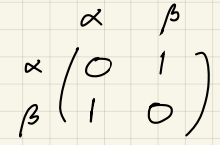
\includegraphics[width=0.15\textwidth]{IntersectionFormS2xS2.png}\end{center}
``So this neat little matrix that you can think of is like an extra invariant of your manifold, which you could use to distinguish manifolds that maybe had the same cohomology groups.''
\end{exmp}
\end{section}
\begin{section}{Lecture 14: Compactly Support Cohomology}
In which we meet another form of cohomology. ``We need open balls in $\Real^n$ to carry cohomological information.''\\
Let $\man$ be a manifold, and $\Recall$ $\compactpformman{p} \coloneqq \{ \omega \in \pformman{p} : $ supp $\omega$ is compact$\}$, where supp $\omega \coloneqq \overline{\{x\in \man : \omega(x) \neq 0\}}$.\\
We have $\deriv : \compactpformman{p} \to \compactpformman{p+1}$, and $\deriv^2 = 0$.
\begin{defn}
The $p^th$ compactly supported cohomology group is 
$$H^p_c(\man) \coloneqq \Ker (d : \compactpformman{p} \to \compactpformman{p+1}) / \Ima(d : \compactpformman{p-1} \to \compactpformman{p})$$
for $p\geq 0$.
\end{defn}
\begin{exmp}
Let $\man$ be non-compact and connected. Then $H_c^0(\man) = 0$
\end{exmp}
\begin{proof}
$\compactcohomman{p} = \{ f$ constant on $\man$ and compactly supported$\}$, and if $\man$ is non-compact, then supp$f \subset \man$ so $f = 0$.
\end{proof}
Does compactly supported cohomology give us functoriality like the usual de Rham cohomology? The first step is figuring out if we can pullback along $f$ and get a compactly supported form in a commutative way. If $f:\man \to \nan$ smooth map of manifolds and $\omega \in \compactpformnan{p}$, then $f^*\omega \in \pformman{p}$, and supp $f^*\omega \subset f^{-1}($supp$\omega$). When is this compact?
\begin{defn}
We say $f:\man \to \nan $ is $\textbf{proper}$ if for all compact $K \subseteq \nan, \, f^{-1}(K)$ is compact.
\end{defn}
Thus if $f$ is proper, we have $f^{-1}($supp$\omega$) compact hence supp$f^*\omega$ compact and we get $f^*: \compactpformnan{p} \to \compactpformman{p}$, and an induced map $f^* : \compactcohomnan{p} \to \compactcohomman{p}$, which is an isomorphism when $f$ is a diffeomorphism (inherited from de Rham cohomology).
\begin{defn}
Let $\man_0, \man_1$ be manifolds without boundary and let $f_i: \man_0 \to \man_1$ be smooth for $i=0,1.$ We say $f_0,f_1$ are $\textbf{properly smooth homotopic}$ if there exists a smooth $H: \inter \times \man_0 \to \man_1$ proper such that $H(0,x) = f_0(x)$ and $H(1,x) = f_1(x)$.\\
We say $\man_0$ and $\man_1$ are $\textbf{properly smoothly homotopy equivalent}$ if there exists smooths $f: \man_0 \to \man_1, g: \man_1 \to \man _0  \st f\circ g \sim \id_{\man_1}, g\circ f \sim \id_{\man_0}$ where the equivalences are properly homotopic. 
\end{defn}
\begin{prop}
If $\man_0,\man_1$ are properly smoothly homotopy equivalent, then $H^p_c(\man_0) \cong H^p_c(\man_1)$.
\end{prop}
\begin{semiproof}
Proof is very similar to proof of Proposition \ref{prop:homotopyequivalenceimpliescohomologyequivalence}.
\end{semiproof}
\begin{subsection}{Pushforwards}
Let $U\subseteq \man$ be open and $i : U\hookrightarrow \man$. Then we have pushforwards\footnote{Mnemonic for where the star goes: You kick things forwards, you pull things back with your hands.}:
$$i_* : \Omega_c^p(U) \to \compactpformman{p}, \quad p \geq 0$$
Let $\omega \in \compactpformman{p}$. Then define $i_* \omega = \begin{cases}\omega, & \text{ on } U\\ 0, & \text{ on } \man \backslash U \end{cases}$ (extension by zero), which we can do because $\omega$ is compactly supported. If $V \xhookrightarrow{i} U \xhookrightarrow{i} \man$ then $(i \circ j )_* = i_* \circ j_*$, tautologically.
\end{subsection}
\begin{lemma}
Let $i : U \hookrightarrow \man $ be an immersion such that $U$ is open. Then for all $p \geq 0,$
$$% https://tikzcd.yichuanshen.de/#N4Igdg9gJgpgziAXAbVABwnAlgFyxMJZABgBpiBdUkANwEMAbAVxiRAB12B5AWxgHM6AAgD6AYyEA9NEIAUAVQCUQkAF9S6TLnyEUZAIxVajFm068BdcZOBoA1PtULFajSAzY8BIvvJH6zKyIHNx8gtZospw8dDgAFmKMwACyqi7qmp46PqSG1AGmweZhVmI29o5R7DHxiQwpaWpGMFD88ESgAGYAThA8SGQgOBBIAEz5JkEgWCIAVK5dvf2Ig8NIvsaBbFALID1969RriADME1vBM-MZe0tjRyOn54UgO6oUqkA
\begin{tikzcd}
\Omega _c ^p (U)  \arrow[r, "i_*"] \arrow[d, "d"]  \arrow[dr,phantom,"\circlearrowright"]& \Omega_c^p(\mathcal{M}) \arrow[d, "d"] \\
\Omega_c^{p+1}(U) \arrow[r, "i_*"]                & \Omega_c^{p+1}(\mathcal{M})           
\end{tikzcd}$$
this diagram commutes.
\end{lemma}
\begin{proof}
$$\deriv(i_*(\omega))= i_* \omega = \begin{cases}\deriv\omega, & \text{ on } U\\ 0, & \text{ on } \man \backslash U \end{cases} = i_* \dw$$
So if $\omega$ is closed then $\dw = 0.$ Then $d(i_*\omega) = i_* \dw = 0$ so $i_*$ is closed. Similarly for exactness. For $U \hookrightarrow \man $ as before, we thus get $i_* : H^p_c(U) \to H^p_c(\man)$ for $p \geq 0$. Notice that this (unusually) goes in the same direction as the morphism!
\end{proof}
\begin{prop}[Compactly supported cohomology of punctured manifold]
Let $\man $ have dimension $n$. Write $\puncman \coloneqq \man \backslash \{x\}$ for some fixed $\xman$. Then:\begin{enumerate}
    \item for all $p \geq 2$, $i_* : H^p_c(\puncman) \to \compactcohomman{p}$ is an isomorphism.
    \item if $\man$ compact, then for $p\geq 1, i_* : H_c^p(\puncman) \to \compactcohomman{p} \cong\cohomman{p}$ is an isomorphism (last isomorphism coming from $\compactpformman{p} \cong \pformman{p}$ for compact $\man$).
\end{enumerate}
\end{prop}
``The cohomology of compact manifolds have various nice properties... working with cohomology with compact supports is a way of forcing... manifolds to behave as if they were compact with respect to their cohomology... even if its not [compact].'' The second point will make Poincar\`e Duality (which we will prove later) incredibly powerful, essentially showing cohomology groups are symmetric.
\begin{proof}
\underline{Injectivity:} Let $p\geq 2$. Let $\omega \in \Omega_c^p(\puncman)$ closed $\st i_*[\omega] = 0.$ So $[i_* \omega] = 0$ on $\compactcohomman{p}$, i.e. $\exists \eta \in \compactpformman{p} \st \deta = i_* \omega.$ By Poincar\'e Lemma, $\exists U \subseteq \man$ open s.t. $x\in U$ and $H^p(U) = 0.$ Now supp $i_*\omega \not\ni x$ and supp$i_* \omega$ is closed so $\exists$ nbd of $x$ on which $i_*\omega = 0$, therefore $\eta$ is closed on this nbd. Thus making $U$ smaller, $\eta$ closed, hence exact since $H^{p-1}_c(U) = 0$. So $\exists \sigma  \in \Omega^{p-2}(U) \st \eta = \deriv \sigma$. Let $\{f_U, f_{\puncman}\}$ be a partition of unity wrt open cover of $\man$, $\{U,\puncman\}$. Then let $\eta' = \eta - \deriv(i_*f_U \sigma)$.
\begin{center}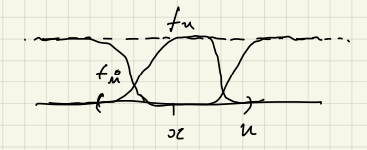
\includegraphics[width=0.45\textwidth]{PuncturedManifoldProposition.png}\end{center}
Now supp$f_{\puncman}\subseteq \puncman$, so $\exists$ nbd of $x$ on which $f_{\puncman} = 0$ and therefore on this nbd, $f_U = 1.$ So on this nbd of $x$, $i_*f_U \sigma = \sigma$. Therefore, on $U$, $\eta' = 0.$ So $\exists \eta' \in \Omega_c ^{p-1} (\puncman) \st \deta ' = \deta = \omega,$ so $[\omega] = 0$ (i.e. $\Ker i_* = 0$ therefore $i_*$ is injective).\\
Now let $p = 1.$ Let $\omega \in \Omega_c^1(\puncman) $ closed s.t. $i_* [ \omega ] = 0.$ Then $\exists f \in \Omega_c^0(\man)$ s.t. $i_*\omega = \df$. By taking $U \subseteq \man $ open s.t. $x\in U$, may assume $\df = 0$ on $U$, as above. So $f = c$ on $U$ i.e. $f\restrict{U}$ is constant. Let $\eta' = \eta -c$. Then $\eta' = 0$ on $U$ and so if $\man$ is compact then $\eta' \in \Omega_c^0(\puncman)$; thus $\omega = \deta' $ and $[\omega] = 0$.\\
\underline{Surjectivity:} ($p\geq 1)$ Let $\omega \in \compactpformman{p}$ closed. By Poincar\'e Lemma, $\exists U \ni x \st \omega \restrict{U} $ is exact. So $\exists \sigma \in \Omega^{p-1}(U) \st \deriv \sigma = \omega \restrict{U}.$ Let $\{f_U, f_{\puncman}\}$ be as above, and let $\omega' = \omega - \deriv(i_* f_U \sigma)$. Then $\omega ' = 0 $ on a nbd of $x$ and $[\omega ] = [\omega ' ].$ And $\omega ' \restrict{\puncman} \in \Omega_c^p(\puncman).$ Thus $[i_*\omega' \restrict{\puncman}] = [\omega'] = [\omega].$
\end{proof}
\begin{exercise}
Compute $H^1_c(\Real^2 \backslash \{0\})$ by hand.
\end{exercise}
\begin{exmp}
$H_c^p(\Real^n) = \begin{cases} \Real, & p = n \\ 0 ,& \text{o/w} \end{cases}$
\end{exmp}
\begin{proof}
$\Real^n \cong S^n \backslash \{x\}$ so by Proposition, $H^p_c(\Real^n) \cong H^p_c(S^n)$ for $p\geq 1$. So $H^p_c(S^n) \cong H^p(S^n)$ which we know from MVT. So $H^p_c(\Real^n) = \begin{cases} \Real, & p = n \\ 0 ,& 1\leq p < n \end{cases}$. And $H^0_c(\Real^n) = 0$ because $\Real^n$ is not compact.
\end{proof}




\end{section}
\begin{section}{Lecture 15: Poincar\'e Duality}
Roughly speaking, when $\man$ is an orientable manifold, Poincar\'e duality says is that $\cohomman{p} \cong \compactcohomman{n-p}^*$, where $n = \dim \man$ and this isomorphism has some geometric meaning.\\
$\Recall$ $\cohomman{p} \times \cohomman{q} \to \cohomman{p+q} : ([\omega],[\eta]) \mapsto ([\omega \wedge \eta] )$ is wel-defined and $[\omega] \wedge [\eta]  = (-1)^{pq}([\eta]\wedge [ \omega])$.
\begin{lemma}
$\man$ oriented without boundary of dimension $n$. Then there exists a linear map 
$$I_\man : \compactcohomman{p} \to \Real: [\omega] \mapsto \int_\man \omega$$
which is surjective. We call this map `integration'.
\end{lemma}
\begin{proof}
If $\omega \in \compactpformman{n}$ exact then by Stokes' Theorem $\int_ \man \omega = 0$, so $I_\man$ is well-defined as it is vanishing at boundaries. It's linear because integration is linear. For surjectivity, we need to find some $\omega \in \compactpformman{p}$ closed s.t. $\int_\man \omega \neq 0$. Since $\man$ is oriented, there exists a volume form $\omega_0 \in \pformman{n} $. Take $f\in \cts{\man}$ compactly supported with $F \geq 0$. Let $\omega = f \cdot \omega_0 \in \compactpformman{n}.$ And $\compactpformman{n+1} = 0$, so $\omega$ is closed. And $\int_\man \omega = \int_\man f \cdot \omega_0 > 0 $ because $\int_\man \omega_0 > 0.$
\end{proof}
\begin{exmp}
$\man = S^n$. Let $\omega \in \compactpformman{n} \st \int_{S^n} \omega = 0.$ We want to show that $\omega$ is exact (so that the integral is 0 by Stokes' and then we can say that $I_\man$ is injective). Since $\man$ is compact, $\compactcohomman{n} \cong \cohomman{n} = \Real$. Alongside $I_\man$ is linear and surjective we must have that it's injective. So $[\omega]=0$. 
\end{exmp}\noindent
Let $\man$ be connected manifold of dimension $n$. Then take $q = n-p$. We have: 
$$
\cohomman{p} \times \compactcohomman{n-p} \to \compactcohomman{n} \to \Real$$
$$([\omega],[\eta]) \mapsto [\omega \wedge \eta] \mapsto \int_\man \omega \wedge \eta$$
This map is bilinear (need to check that if $\eta$ has compact support then so does $\omega \wedge \eta$, but this is easy). When $\varphi : V \times W \to \Real$ is bilinear, we get 
$$V \to \HomReal{W}{\Real}: v \mapsto \varphi_v$$
where $\varphi_v : V \to \Real: w \mapsto \varphi(v,w)$. Thus we get linear map $$\Phi : \cohomman{p} \to \compactcohomman{n-1} ^*:\omega \mapsto (\eta \mapsto \int_\man \omega \wedge \eta)$$. Poincar\'e duality says that this is an isomorphism (the geometric part comes from integration over submanifolds, and we'll see more of that towards the end of the course after we see singular (co)homology).

\begin{exmp}(Base case for Poincar\'e Duality)
$U \subseteq \Real^n$ open subset diffeomorphic to $\Real ^n$. Then $\cohom{p}{U} = \begin{cases} \Real,& p= 0\\ 0,& p > 0\end{cases}$ and $ H^p_c(U) = \begin{cases} 0,& p<n\\ \Real,& p =n\end{cases}$, as we saw in last lecture. To check the given Poincar\'e duality map is an isomorphism, it's enough to check $p = 0$, and enough to check injectivity. That is, we must check $\exists \omega \st \Phi(\omega) \neq  0.$ Given $\omega \in H^0(U)$, $\Phi: H^n_c(U) \to \Real : \eta \mapsto \int_U \omega \wedge \eta$. But $[\omega] \in H^0(U)$ so $\omega$ is a constant function on $U$. Say $\omega = c \in \Real$, so $\Phi(\omega) : H^n_c(U) \to \Real : \eta \mapsto c\cdot \int_\man \eta$, and $\exists \eta \st \int_\man \eta \neq 0$, by the above lemma. So Poincar\'e Duality holds in the simplest possible case.
\end{exmp}
\end{section}


\begin{section}{Lecture 16: Proving Poincar\'e Duality}
\begin{theorem}[Poincar\'e Duality]\label{theorem:PoincareDuality}
Let $\man$ be an oriented manifold of dimension $n$. Then the map $\Phi : \cohomman{p} \to \compactcohomman{n-p}^*$ is an isomorphism.
\end{theorem}
We will prove this only for a smaller class of `nice' manifolds which includes compact ones.
\begin{defn}
We say $\man$ is of finite type is $\exists$ finite open cover of $\man$ by sets $\{U_i\}$ s.t. for all $k \geq 1,$ $U_{i_1} \cap ... \cap U_{i_k}$ is either empty of diffeomorphic to $\Real^n$.
\end{defn}
Contrast that with the definition of a good cover. It's a fact that compact manifolds are of finite type\footnote{John M. Lee's Introduction to Smooth Manifolds talks more about the non-finite type case.}.
\begin{exercise}
Show that $\Real^2 \backslash \mathbb{Z}$ is not of finite type (Hint: $\dim H^1(\Real^2 \backslash\mathbb{Z}) = \infty)$
\end{exercise}\noindent
``If a manifold is of finite type, then all of its de Rham cohomology groups are finite dimensional''.
\\Idea for proving Poincar\'e Duality: Use induction on the size of the cover $\{U_i\}$ along with Mayer-Vietoris and the five lemma\footnote{``This isn't the proof that Poincar\'e originally gave by the way, this is using machinery that was developed quite a way long after Poincar\'e was working.''}. For that we need a version of MVT for compactly supported cohomology.
\begin{prop}
Let $\man = U \cup V$ where $U,V$ open and $U\cap V \neq \varnothing$. Then $\exists$ short exact sequence of cochain complexes:
$$% https://tikzcd.yichuanshen.de/#N4Igdg9gJgpgziAXAbVABwnAlgFyxMJZABgBoBGAXVJADcBDAGwFcYkRiQBfU9TXfIRTkK1Ok1bsAOlIDyAWxgBzegH0AxgD00ACgCqM9fTQACAGoBKbrxAZseAkQBMomgxZtEIGQuVqtunoWJjIARlhKEGgscCFyiioa2jqW1nz2gkQAzK7iHtLxfkm6MvL0OAAWRozAALJcVjzpAo4oACy57pJenE22-A5CyCJOYl2eIAB002n9Ga3ILqNuEhPTk7N2LUM5y3ndUzN9W4PZpMRjq+zrmwOZKC4XK-leN8d3CyJP+2tHYjBQJTwIigABmACcIPIkGQQDgIEhyH0IVDETR4UgXD92AArWYo6GILEYxA5bFeLD4yGEskktrI6lIAAc6IRpIZqMQAE5WZiOYTyLCSUibAS0XC2QBWfmY3mIABsMtJcoA7FxKFwgA
\begin{tikzcd}
            & ... \arrow[d]                                & ... \arrow[d]                                                  & ... \arrow[d]                               &   \\
0 \arrow[r] & \Omega_c^p(U\cap V) \arrow[r, "j"] \arrow[d] & \Omega_c^p(U) \bigoplus \Omega_c^p(V) \arrow[r, "i"] \arrow[d] & \Omega_c^p(\mathcal{M}) \arrow[r] \arrow[d] & 0 \\
            & ...                                          & ...                                                            & ...                                         &  
\end{tikzcd}$$
where 
$$% https://tikzcd.yichuanshen.de/#N4Igdg9gJgpgziAXAbVABwnAlgFyxMJZABgBoBGAXVJADcBDAGwFcYkQBVEAX1PU1z5CKcqWLU6TVuw4AdWQGN6aAAQA1HnxAZseAkQBMFCQxZtEIDb366hRUQZNTzIeQFt6OABZLGwALLcPBIwUADm8ESgAGYAThBuSGQgOBBIAMw0OPRYjOxeEBAA1iA0ptIWWAD6XNYgcQlIoilpiEYpOXkWBcWlkmbsAFZVGjSM9ABGMIwACgJ6wiCxWGFeOJox8YmIzalJWZ35hSVlzkM1G-VbSO17iJkduUe9pwOVI33jU7PzdhbLq3W3Eo3CAA
\begin{tikzcd}
                          & U\cap V \arrow[rd, "j_V"', hook] \arrow[ld, "j_U", hook] &                            \\
U \arrow[rd, "i_U", hook] &                                                          & V \arrow[ld, "i_V"', hook] \\
                          & \mathcal{M}                                              &                           
\end{tikzcd}$$
and $i = i_{U*} + i_{V*}, \, j= (-j_{U*},j_{V*})$
\end{prop}
\begin{proof}
$j$ injective: If $\omega \in \Omega^p_c(U\cap V) \st j(\omega) = 0 $ then $ j_{U*} \omega = j_{V*} \omega= 0 $. So $\omega = 0$.\\
$\Ker i = \Ima j:$ Let $\omega \in \Omega^p_c(U\cap V)$. Then $i \circ j (\omega) = - i_{U*} j_{U*} + i_{V*} j_{V*} \omega = 0$. So $\ima j \subseteq \Ker i$. Now let $(\omega_1,\omega_2) \in \Ker i$. Then $i_{U*} \omega_1 = -i_{V*} \omega_2$ so supp $\omega_1,\omega_2 \subset U\cap V$. So $\exists \eta \in \Omega_c^p(U\cap V) \st j_{U*}\eta = -\omega_1, j_{V*} \eta = \omega_2$. So $j(\eta) = (\omega_1,\omega_2).$ So $\Ker i \subseteq \Ima j$. \\
$i$ surjective: Let $\omega \in \Omega_c^p(\man)$ and let $\{f_U,f_V\}$ be a partition of unity wrt $\{U,V\}$. Define $\omega_U \coloneqq f_U \cdot \omega\restrict{U} \in \Omega_c^p(U)$ and $\omega_V \coloneqq f_V \cdot \omega\restrict{V} \in \Omega_c^p(V)$. Then $i(\omega_U,\omega_V) = \omega$.\\
Therefore this is a short exact sequence on each row.
\end{proof}
\begin{corollary}[Mayer-Vietoris for Compact Supports]\label{cor:CompactMVT}
There is a long exact sequence
$$\begin{tikzcd}
... \arrow[r] & H_c^p(\UintV) \arrow[r, "f"]     & H_c^p(U)\oplus H_c^p(V) \arrow[r, "g"]         & H_c^p(\mathcal{M}) \arrow[lld, "\delta_c",bend right = 5] &     \\
              & H_c^{p+1}(\UintV) \arrow[r, "f"] & H_c^{p+1}(U)\oplus H_c^{p+1}(V) \arrow[r, "g"] & H_c^{p+1}(\mathcal{M}) \arrow[r, "\delta_c"]                          & ...
\end{tikzcd}$$
NB that the order is different than for the usual Mayer-Vietoris sequence.
\end{corollary}
\begin{proof}
Just like for the usual case, this is an immediate consequence of the Snake lemma.
\end{proof}
We will be putting the compact MV sequence ``on top of'' the usual MV sequence, but in order for the arrows to go the same way, we will take the dual of the former to reverse them. First we have to prove that's what taking the dual does though.
\begin{lemma}
Let $C_1 \xrightarrow{f_1} C_2 \xrightarrow{f_2} C_3$ be an exact sequence of vector spaces. Then the dual sequence $C_1^* \xleftarrow[]{f_1^*} C_2^* \xleftarrow[]{f_2^*} C_3^*$ is also an exact sequence. Here $f_i^*$ represents the dual linear map, not the pullback.
\end{lemma}

\noindent
$\Recall$ Given $(\varphi : C_2 \to \Real ) \in C_2^*$, $f_1^*( \varphi)\in C_1^*$ is $f_1^*(\varphi) : C_1 \xrightarrow[]{f_1^*(\varphi)} \Real: v\in C_1 \mapsto f_1(v) \in C_2 \mapsto \varphi(f_1(v))\in \Real$.

\begin{proof}
We have $\Ker f_2 = \Ima f_1$; want to show $\Ker f_1^* = \Ima f_2^*$. Given some $\varphi \in \Ker f_1^*$. Then $\varphi \circ f = 0,$ so $\Ker f_2 = \Ima f_1 \subset \Ker \varphi$. So $\exists \bar{\varphi} : C_2 / \Ker f_2 \to \Real$. And $C^2 /\Ker f_2 \cong \Ima f_2 \subset C_3$, so we can extend $\bar{\varphi} $ to $\psi : C_3 \to \Real, \st \psi \circ f_2 = \varphi$. So $f_2^*(\psi) = \varphi, \ie \varphi \in \Ima f_2^*.$\\
Now let $\varphi \in \Ima f_2^*.$ Then $\exists \psi \in C_3^* \st f_2^*(\psi) = \varphi, \ie \psi \circ f_2 = \varphi.$ And $0 = \psi \circ f_2 \circ f_1 = \varphi \circ f_1 = f_1^*(\varphi).$ Hence $\varphi \in \Ker f_1^*$.
\end{proof}


\begin{proof}[Proof of Thm $\ref{theorem:PoincareDuality}$]
Let $\man$ be finite type oriented manifold with cover $\{U_i\}$. Let $N = \#\{U_i\}$, $n = \dim \man$. We'll prove this by induction on $N$. For $N = 1$, we're ok; an open set of $\Real^n$ diffeomorphic to $\Real^n$ satisfies PD by the example from last lecture. Now suppose $N > 1$, and let $U = \bigcup\limits_{i=1}^{N-1} U_i, V = U_N$. So $\man = U \cup V$. Furthermore, if $\man$ is connected then $U\cap V \neq \varnothing$. If $\man$ is not connected, work with each connected component separately (there are only finitely many because $\man$ is finite type). So let's just assume $\man$ is connected. By induction, can assume $U, V \myand U\cap V$ all satisfy PD. Combine this with MV and the dual of compactly supported MV:
$$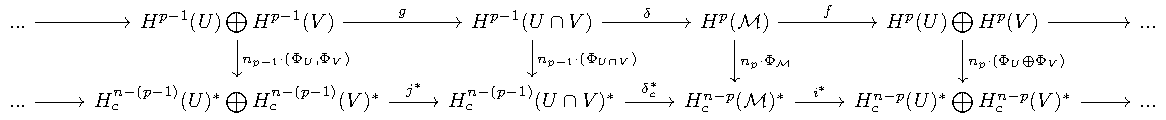
\includegraphics[page=1,width = \textwidth]{PoincareDualityProofDiagram.pdf}$$

with $j^*,i^*$ representing the duals of the inclusion maps (on the cochain complexes) on cohomology. The vertical arrows will be the PD isomorphism maps\footnote{``But, it turns out, for reasons that are, to be honest, somewhat mysterious, if you want these diagrams to commute, you have to introduce a correct sign, a correct factor of minus 1.''}, we hope. For this, let $n_0 = 1$ and $n_p = (-1)^{p-1}n_{p-1}$. The vertical arrows are then given as in the diagram. The effect of this is to correct that without them, the center square only commutes up to sign (the other two squares do commute anyway though).\\
By the Five Lemma, if all vertical maps except from $n_{p-1}\Phi_\man$ are isomorphisms, then so is $n_{p-1}\Phi_\man$ (and hence so is $\Phi_\man)$. Induction tells us that this is the case, except we must also check that all the squares commute\footnote{``This proof ... for some reason, it actually takes a little bit of effort to unwind everything and show that the diagram actually does commute [unlike others we've seen in this course].''}. We'll have to do each square one at a time. NB we ignore the $n_{p-1}$ and $n_p$ terms in 1. and 3. because it would cancel out anyway, being on both sides of the square.\\

1. \underline{$\Phi_{\UintV} \circ g = j^* \circ (\Phi_U \oplus \Phi_V)$:}
$$% https://tikzcd.yichuanshen.de/#N4Igdg9gJgpgziAXAbVABwnAlgFyxMJZABgBpiBdUkANwEMAbAVxiRADpOQBfU9TXPkIoAjOSq1GLNgAkAesDQBaEdwAUAVQCUAHR0AjLAHMIaZnAAE8xSvUA1LTz4gM2PASIAmcdXrNWiCDWyqqaegDGdGgWDk78bkJEAMw+kv5snOxxLgLuwiSkIhJ+0oGZ2a6CHqKFxVIBQQpgSmohWtwA+uGaWnIAVHqGJmZMltbNrSrtXWoO-RW5iSjeRb71sk0tbZ3dGhFRMb19CwnVyCmraaUcXNwSMFBG8ESgAGYAThAAtkhkIDgQJBiK4BMBMBgMagMOj6GAMAAKi2qIAYMFeOGyH2+QOoAKQ3hBbCMIChMLhiNOwhRaIxvDenx+iGBeMQAFY1ulAmAOjZVBEoBAcGo9PCABZYDoaUgi8UdWKk2EIpFU1HozEM-G4wGIFKEwJ6WAMHB0EkoslKylsVW05xYxkElkANg5125vO4-MFwp0YolwD2Oki0Ts3EcCvJyqtNPV2MQABYtUh2XqwRDwxaqiro3SQHak4nEM69SAAFbzdMUzNRtU5vOFgsAdhdDQNcONXVN0MVlby1dpFG4QA
\begin{tikzcd}
... \arrow[r] & H^{p-1}(U)\bigoplus H^{p-1}(V) \arrow[r, "g"] \arrow[d, "{n_{p-1}\cdot(\Phi_U,\Phi_V)}"] & H^{p-1}(U\cap V) \arrow[r, "\delta"] \arrow[d, "n_{p-1}\cdot(\Phi_{U\cap V})"] & ... \\
... \arrow[r] & H^{n-(p-1)}_c(U)^*\bigoplus H^{n-(p-1)}_c(V)^* \arrow[r, "j^*"]                          & H^{n-(p-1)}_c(U\cap V)^* \arrow[r, "\delta_c^*"]                                 & ...
\end{tikzcd}$$
Let $\omega_U \in \Omega^{p-1}(U)$ and $\omega_V \in \Omega^{p-1}(V)$ be closed (the representatives of classes in cohomology). We must show that for any $\eta \in H^{n-(p-1)}_c(\UintV)$, we have 
$$\Phi_{\UintV} \circ g([\omega_U,\omega_v])(\eta) = j^*(\Phi_U([\omega_U]),\Phi_V([\omega_V]))(\eta)$$
an equality of real numbers. Recall $g \coloneqq j_V^* - j_U^*.$ Then $\int_{\UintV} g(\omega_U,\omega_V) \wedge \eta = - \int_U \omega_U\wedge j_{U*} \eta + \int_V \omega_V \wedge j_{V*}\eta$, which you can see is the RHS if you stare at it for a bit.\\
\noindent
3. \underline{$(\Phi_U\oplus\Phi_V) \circ f = i^* \circ \Phi_\man$:}
$$% https://tikzcd.yichuanshen.de/#N4Igdg9gJgpgziAXAbVABwnAlgFyxMJZABgBpiBdUkANwEMAbAVxiRADpOQBfU9TXPkIoAjOSq1GLNgAkAemgAUAHWUBbOjgAWAY0bAAstwCUPPiAzY8BIgCZx1es1aIQ8pQFVjAAlUAjLABzCDRmOG93RQA1U15+KyEiAGYHSWc2TnYzeMEbFDIRCSdpV0zsiwFrYWQxQscpFzc5YDAAWjRuAH0dFXVNXX0jYzkAKnLLXOr7OrSSt27mto7FL1HfZQDg0KZwmQWW9u5o4bG4ioS85BSZ4say7gkYKED4IlAAMwAnCDUkMhAcBAkGJZo1VLAGDg6CBqAw6H4YAwAAqVRKuBgwd44cpfH7A6iApD2UFsd4wkBwhHI1F5CmY7FnXG-RAgwmIACs9XSrjAnTQ6x0UAgOHWSK0WF6Gm0egYhhM5MpiJRF2EdKxOO+zOJbJSJMQYCYDAYsPhSppqox6sZmqJBKBiAAbFy5ry0KpBcLemKsJ0POsQmFReLOjEFabqSq2JaGeYmUgACx2pCcvUgcGIqELMYmqnKyZR+kavEcpOO52NLCjMO580Fq2xm1lgH2gDs5aQBqNObNkfRhYe3CAA
\begin{tikzcd}
... \arrow[r, "\delta"]     & H^p(\mathcal{M}) \arrow[r, "f"] \arrow[d, "n_p \cdot \Phi_\mathcal{M}"] & H^p(U) \bigoplus H^p(V) \arrow[r] \arrow[d, "n_p\cdot(\Phi_U \oplus \Phi_V)"] & ... \\
... \arrow[r, "\delta_c^*"] & H^{n-p}_c(\mathcal{M})^* \arrow[r, "i^*"]                                & H_c^{n-p}(U)^* \bigoplus H_c^{n-p}(V)^* \arrow[r]                             & ...
\end{tikzcd}$$
i.e. for all $\omega \in \Omega^p(\man) $ and all ($\eta_U,\eta_V) \in \Omega_c^{n-p}(U) \oplus \Omega_c^{n-p}(V)$ closed, we have 
$$\int_U \omega\restrict{U} \wedge \eta_U + \int_V \omega\restrict{V} \wedge \eta_V = \int_\man \omega \wedge i(\eta_U,\eta_V)$$
This falls out from the definition of $i$ as $i_{U*} + i_{V*}$ pretty automatically.
\\
2. \underline{$n_p \cdot \Phi_\man \circ \delta = \delta_c^* \circ n_{p-1} \cdot \Phi_{\UintV} $:}
$$% https://tikzcd.yichuanshen.de/#N4Igdg9gJgpgziAXAbVABwnAlgFyxMJZABgBpiBdUkANwEMAbAVxiRADpOQBfU9TXPkIoAjOSq1GLNgAkAesDQBaEdwAUAVQA6WgMZ00AAgBqASh58QGbHgJEATOOr1mrRCHlo1OgLZ0cABb6DMAAstzmvPw2QkQAzE6Srmyc7BbRgnYoZCISLtLuqelWArbCyGK5zlJuHgpgSmrKIqbcAPq6mjr6RmZyAFTF1pnljlVJBXXADWjtnb7+QYxhEQNDpbEoCeP5tUXcEjBQAObwRKAAZgBOED5IZCA4EEhiE7XHINQMdABGMAwABQ2WRADBgFxwxWutxe1CeSEcbzYOlgDBwdE+oN+-yBMRBYIhUJud0Qr3hiAArNVku4wG1FCpuN0oBAcN4tACAlh6do9AYTBFMd8-oDgcJQeDIVEQNCSYjyQkke4LkLsaK8eKCVLLLKEXDnogAGzUyZ0ozM1mGHScrDsvyBYIrcxfNW4kZsLVEmGIAAs+qQVKVIAAVmsXSK3WUPZKvSTA+TjUGUf90R1VRGxdHCdLdUb-YgAOwm2pYMNYjMarNSijcIA
\begin{tikzcd}
... \arrow[r, "g"]   & H^{p-1}(U\cap V) \arrow[r, "\delta"] \arrow[d, "n_{p-1}\cdot(\Phi_{U\cap V})"] & H^p(\mathcal{M}) \arrow[r, "f"] \arrow[d, "n_p \cdot \Phi_\mathcal{M}"] & ... \\
... \arrow[r, "j^*"] & H^{n-(p-1)}_c(U\cap V)^* \arrow[r, "\delta_c^*"]                                 & H^{n-p}_c(\mathcal{M})^* \arrow[r, "i^*"]                                & ...
\end{tikzcd}
$$
This is a lot more difficult because it hinges on the question: What are $\delta_c$ and $\delta$? They both came into this world implicitly from the Snake lemma, so the first goal is to explicit-ize them. Let $\omega\in \compactpformman{p} $ be closed and let $\{f_U,f_V\}$ be a partition of unity wrt $\{U,V\}$. Define $\omega_U \coloneqq f_U \cdot \omega\restrict{U} \in \Omega_c^p(U) ;\;  \omega_V \coloneqq f_V \cdot \omega\restrict{V} \in \Omega_c^p(V) $. Then $i(\omega_u,\omega_V) = i_{U*}\omega_U + i_{V*}\omega_V = \omega_U + \omega_V = \omega.$ If $\omega$ is closed, then $i(\dw_U,\dw_V) = 0$, so $(\dw_U,\dw_V) \in \Ker i = \Ima j$. Since $j$ is injective (on the level of cochain complexes), $\exists ! \delta_c(\omega) \in \Omega_c^{p+1} (\UintV) \st j(\delta_c(\omega)) = (\dw_U,\dw_V)$. And since $f_U + f_V = 1, \df_U = -\df_V$. Now $j(\delta_c(\omega)) = (\dw_U,\dw_V) = (\df_U \wedge \omega\restrict{U} , \df_V\wedge \omega\restrict{V}) = (-\df_V \wedge \omega\restrict{U} , \df_V\wedge \omega\restrict{V}) = j(\df_V \wedge \omega\restrict{\UintV})$, with the last equality coming from the definition of $j$. Therefore, $\delta_c(\omega) = \df_V \wedge \omega\restrict{\UintV}$ as $j$ is injective. So $\delta_c \Omega_c^p(\man) \to \Omega_c^{p+1}(\UintV).$ Let $\eta \in \Omega_c^p(\man)$, then $\deriv(\delta_c(\man)) = \deriv(\df_V \wedge \eta\restrict{\UintV}) = 0 \wedge \eta\restrict{\UintV} + (-1)^p (\df_V \wedge \deta \restrict{\UintV}) = (-1)^p\delta_c(\deta)$, which explains where the necessity of introducing the $n_p$s come from. So $\delta_c$ takes closed forms to closed forms and exact forms to exact forms. Thus we get $\delta_c : \compactcohomman{p} \to H^{p+1}_c(\UintV) : \omega\mapsto \df_V \wedge \omega\restrict{\UintV} $. This makes the sequence exact by construction. Similarly, $\delta_c : H^p(\UintV) \to \cohomman{p} : \omega \mapsto \begin{cases} \df_V\wedge \omega,& \text{ on } \UintV \\ 0, & \text{ else}\end{cases}$.
\\
Now to show commutativity in the central square i.e. $n_p \cdot \Phi_\man ( \delta([\omega_1])) = n_{p-1}\cdot \delta_c^* (\Phi_\UintV([\omega_1]))$ for $\omega_1 \in \Omega^{p-1}(\UintV)$. That is, for all $\omega_2 \in \Omega_c^{n-p}(\man),$ need 
$$
n_{p-1} \int_\man \delta(\omega_1) \wedge \omega_2 = n_p \int_{\UintV} \omega_1 \wedge \delta_c(\omega_2)
$$
Now, $n_{p-1} \int_\man \delta(\omega_1)\wedge\omega_2 = n_{p-1} \int_\man (\df\restrict{V} \wedge \omega_1 \restrict{\UintV}) \wedge\omega_2 = n_{p-1} \int_{\UintV} (\df_V \wedge \omega_1 \restrict{\UintV} \wedge \omega_2 \restrict{\UintV} = n_p \int_{\UintV} \omega_1 \restrict{\UintV} \wedge \df _V \wedge \omega_2 \restrict{\UintV} = n_p \int_{\UintV} \omega_1 \wedge \delta_c(\omega_2)$, as required. NB the sign change from moving terms in the wedge product. This concludes the proof.
\end{proof}
\begin{corollary}
Let $\man$ be compact, oriented and connected manifold of dimension $n$.
\begin{enumerate}
    \item Then $\cohomman{n} \cong \Real$
    \item We have $b_k(\man) = b_{n-k}(\man) \, \forall k$
    \item Define the Euler characteristic $\chi(\man) \coloneqq \sumfromto{i=0}{n} (-1)^k b_k(\man).$ Then $\chi(\man) = 0$ if $n$ odd.
    \item If $\man$ is of finite type and non-compact, then $\cohomman{n} = 0.$
\end{enumerate}
\end{corollary}
\end{section}


\begin{section}{Lecture 17: Degrees of Proper Maps}

Let $\man$ and $\nan$ be connected manifolds of the same dimension $n$. Poincar\'e duality tells us that $\compactcohomman{n},\compactcohomnan{n}$ have canonical isomorphisms to $\Real$ (choose a differential form and integrate it over the whole manifold to get a real number).
\begin{defn}
If $f:\man \to \nan$ proper smooth, we get $f^*: \compactcohomnan{n} \to \compactcohomman{n}$ a linear map $\Real \to \Real$ i.e. a multiplication by some $c\in \Real$. We define $\deg f = c$.
\end{defn}
This expresses the relation between the integral of a form and the integral of its pullback i.e. if $\omega\in\compactpformnan{n}$ then $\int_\man f^*\omega = \deg f \int_\nan \omega$.
\begin{prop}
If $f : \man \to \nan$ and $g: \nan \to \pan$ are smooth proper maps of orientable manifolds of the same dimension then
\begin{enumerate}
    \item $\deg (g\circ f) = \deg g \cdot \deg f$
    \item If $f$ is a diffeomorphism then $\deg f = +1$ if $f$ is orientation preserving and $\deg f = -1$ if $f$ is orientation reversing.
    \item If $f,g$ are properly smoothly homotopic then $\deg g = \deg f$ ($g : \man \to \nan $ here)
\end{enumerate}
\end{prop}

%tk XXX to do: amke consistent whether youre using thm of theorem enviroment
\begin{thm}\label{thm:DegreeInteger}
$\deg f$ is always an integer.
\end{thm}

\begin{defn}
Let $f:\man\to\nan$. We say $y\in \nan$ is a $\textbf{regular value}$ of $f$ is for all $x\in f^{-1}(y),$ $Df_x$ has full rank. We say $y\in\nan$ is a $\textbf{critical value}$ if it is not a regular value.
\end{defn}
We state these next few powerful theorems without proving this:
\begin{thm}[Sard's Theorem]
The set of critical values of $f : \man \to \nan$ is measure zero in $\nan$, so that $\nan \backslash \{\text{critical values of } f\}$ is dense in $\nan$.
\end{thm}

\begin{thm}[Implicit Function Theorem]
If $x\in \man$ is such that $Df_x$ is an isomorphism, then $\exists U \ni x$ open s.t. $f\restrict{U} : U \to f(U)$ is a diffeomorphism.
\end{thm}

\begin{thm}[Pre-Image Theorem]
Let $y\in \nan$ be a regular value of $f : \man \to \nan$. Then the fibre $f^{-1}(y)$ is a smooth manifold of dimension $\dim \man - \rank Df_x$ where $x\in f^{-1}(y)$.
\end{thm}
NB for the last theorem, we don't assume that $\man$ and $\nan$ have the same dimension, so $Df_x$ may not be an isomorphism.
\begin{center}
    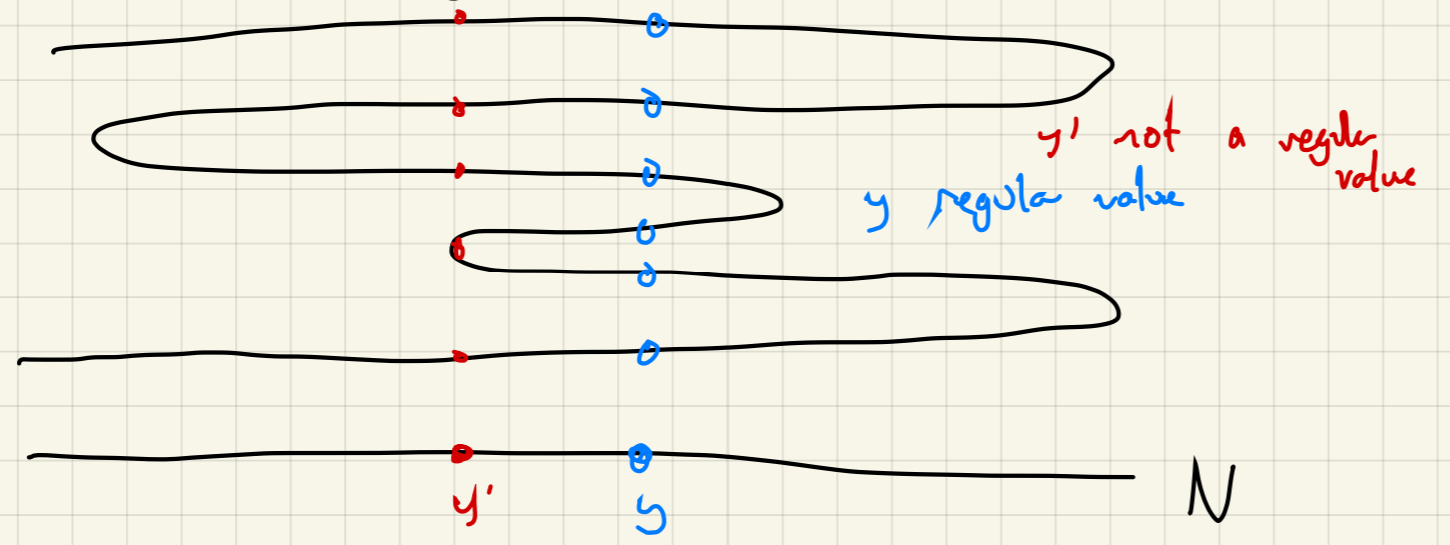
\includegraphics[width =0.5\textwidth]{RegularValues.png}
\end{center}

\begin{proof}[Proof of Thm \ref{thm:DegreeInteger}]
Let $R(f) = \{\xman : \rank Df_x = n\}$. If $R(f) = \varnothing$, then $\deg f = 0$ by direct calculation ($\det Df_x = 0,$ so pullback integral is killed). If $R(f) \neq\varnothing$, take $x \in R(f).$ Then by Implicit Function Theorem $\exists U \ni x$ open in $\man \st f\restrict{U} : U \to f(U)$ is an diffeomorphism. Now $f(U)$ is open so by Sard's theorem $\exists$ regular value $y\in f(U) \subseteq \nan$.\\
Let $f^{-1}(y) = \{\allthe{x}{1}{m} \}$ (fibre is smooth 0-manifold, and $f$ is proper so is compact therefore finite). Each $x_i \in f^{-1}(y)$ has $Df_{x_i}$ isomorphism so $\exists U_i \ni x_i$ open s.t. $f\restrict{U_i}$ is an isomorphism. Shrinking these if necessary, $U_i$ all disjoint and each $U_i \to U$ is a diffeomorphism (shrinking $U$ if necessary).\\
Let $\omega \in \compactcohomman{n}$ be $\st \int_U \omega = 1$ and supp $\omega \subset U$ ($\underline{Exercise:}$ Why does this exist?). Since $f\restrict{U_i}$ is a diffeomorphism, get $\int_{U_i} f^* \restrict{U_i} \omega = \sign \det(Df_{x_i}) \int_U \omega.$ And $f^*\restrict{U_i} \omega$ has support in $U_i$. Since $\supp f^*\omega \subset \bigcup\limits_{i} U_i,$ and all of these $U_i$s are by construction disjoint, $\int_\man f^*\omega = \sumfromto{i=1}{k} \int_{U_i} f^*\restrict{U_i} \omega = \sumfromto{i=1}{k} \sign(\det Df_{x_i}) \int_U \omega = \sumfromto{i=1}{k} \sign (\det Df_{x_i}) \in \mathbb{Z}.$
\end{proof}
\begin{center}
    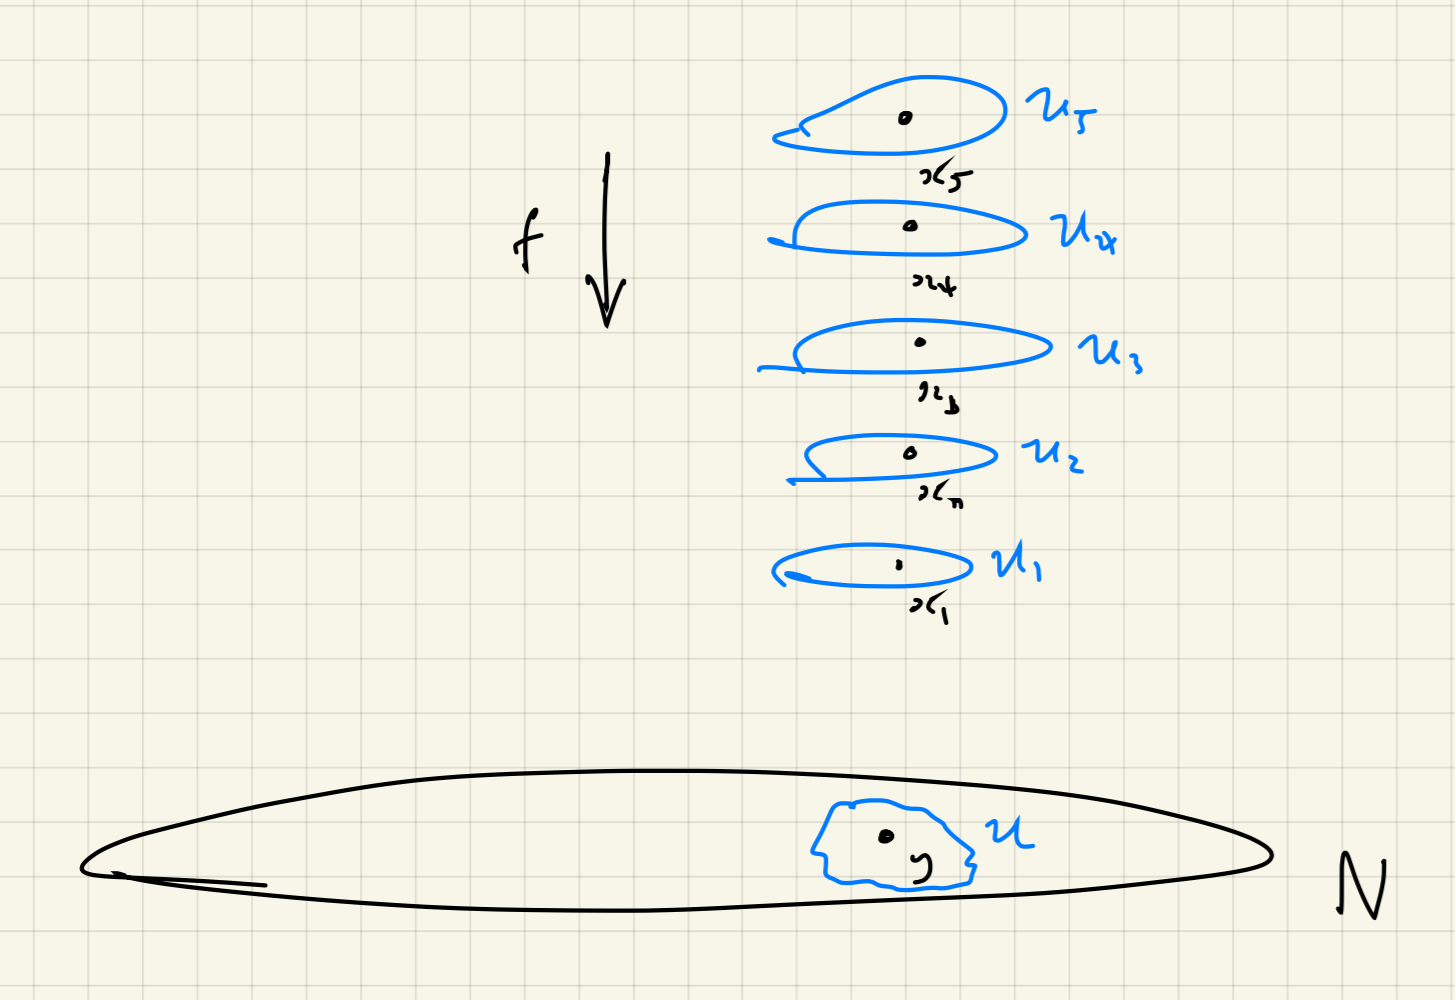
\includegraphics[width = 0.5\textwidth]{DegreeCovering.png}
\end{center}

\begin{exercise}
If $f : \man \to \nan$ is proper between connected oriented manifolds, and $f$ is not surjective, then $\deg f = 0.$
\end{exercise}

\begin{exmp}
$\man = \nan = S^n$, $f:S^n \to S^n : x \mapsto -x$, the antipodal map. Claim: $\deg f = (-1)^{n+1}$. Let $i: S^n \hookrightarrow \Real^{n+1}$, and $\bar{\omega} = x_1 \allthewedge{\dx}{2}{n+1} \in \Omega^n(\Real^{n+1}).$ Then if $\omega = i^* \bar{\omega} \in \Omega^n(S^n). $ By Stokes': $\int_{S^n} \omega = \int_{S^n} i^* \bar{\omega} = \int_{D^{n+1}} \deriv\bar\omega = \int_{D^{n+1}} \allthewedge{\dx}{1}{n+1} \neq 0$. So $f$ can be extended to $\bar f : \Real^{n+1} \to \Real^{n+1} : x \mapsto -x$. Then $\bar f \circ i = i\circ f$ and $f^*\bar\omega = (-1)^{n+1} \bar \omega,$ so $$f^*\omega = f^* i^* \bar \omega = (i\circ f)^* \bar \omega (\bar f \circ i) ^* \bar \omega = i^* \bar f ^* \bar \omega = (-1)^{n+1} i^* \bar \omega = (-1)^{n+1} \omega$$ Thus $(-1)^{n+1} \int_{S^n} \omega = \int_{S^n} f^* \omega = \deg \int_{S^n} \omega$, so $\deg f = (-1)^{n+1}.$
\end{exmp}
\end{section}


\begin{section}{Lecture 18: Cohomology of Complex Projective Space}
This will be the last bit of de Rham cohomology for a while, so let us finish with an extended example.\\
Let $\CProj^n \coloneqq \{z\in\mathbb{C}^{n+1} \remzero\} / (z\sim \lambda z $ with $\lambda \in \mathbb{C} \remzero)$ (complex lines through the origin or all the $n$ dimensional vector subspaces of $\mathbb{C}^{n+1}$). We write $[z_0: z_1: \ldots : z_n] \in \CProj^n$ for the equivalence class of $(z_0,\ldots,z_n) \in \mathbb{C}^{n+1}$. Therefore if $z_n\neq 0,$ we can uniquely write this class as $[\frac{z_0}{z_n}: \ldots : \frac{z_{n-1}}{z_n} : 1 ].$ This gives a homeomorphism $U_{z_n\neq 0} \coloneqq \{ [ z_0 : \ldots : z_n] \in \CProj ^n \st z_n \neq 0\} \xrightarrow[]{\sim} \mathbb{C}^n: [z_0 : \ldots: z_n ] \mapsto (\frac{z_0}{z_n},\frac{z_1}{z_n},\ldots,\frac{z_{n-1}}{z_n}) \in \mathbb{C}^n$. These are called `affine charts' $U_{z_i\neq0} \xrightarrow[]{\sim} \mathbb{C}^n$. Transition maps on $U_{z\neq 0} \cap U_{z_n \neq 0} $ are given by the resultant transformation of 
$$(\omega_0,\ldots,\omega_{n-1}) \mapsto [\omega_0:\ldots : \omega_{n-1} : 1 ] \mapsto \left(\frac{\omega_0}{\omega_{n-1}}, \frac{\omega_1}{\omega_{n-1}},\ldots,\frac{1}{\omega_{n-1}}\right) \in \mathbb{C}^n$$
where $(\omega_0 , \ldots, \omega_{n-1}) \in \mathbb{C}^n$ with $\omega_{n-1}\neq 0$. These transitions are smooth\footnote{They are also biholomorphic, which makes $\CProj$ a complex manifold as well.}.\\
$\Fact$ (Not too hard to prove) If $T_\mathbb{C} : \mathbb{C}^n \to \mathbb{C}^n$ is complex linear, then the associated $\Real$-linear map, $T_\Real : \Real^{2n} \to \Real^{2n}$ satisfies $\det T_\Real = \abs{\det T_\mathbb{C}}^2 \geq 0.$ So any complex manifold is an orientable real manifold. Also, $\CProj^n$ is compact.
\begin{exmp}
$\CProj^1$ is called the `Riemann Sphere': $\CProj \cong \mathbb{C} \sqcup \{\infty\}$, the complex plane ($\{[z:1]\in\CProj^1\}$) with a point at infinity ($[1:0]$) $\cong$ one-point compactification of a plane $\cong S^2$. These are just topological equivalences, but we could get them to carry smooth structural data, so that $S^2$ has a complex structure and is a complex manifold. \\
In general, $\CProj^n = \mathbb{C}^n \sqcup \CProj^{n-1} = \{[z_0:\ldots:z_{n-1}:1]\} \sqcup \{[z_0:\ldots:z_{n-1}:0]\}$\footnote{When any of the coordinates are zero, it's like a degree of freedom is being removed.}.
\end{exmp}

\begin{prop}
$H^p(\CProj^n) = \mycasesthing{ 0,& \myif p \text{ odd}}{\Real, & \myif p \text{ even}} $
\end{prop}
\begin{proof}
Consider $\CProj^n \backslash \{ [0:\ldots:0:1]\} \to \CProj^{n-1} : [z_0: \ldots : z_{n}] \mapsto [z_0: \ldots : z_{n-1}]$. This is a deformation retraction. And by a homework question (Problem sheet 2, exercise 7), $i : \CProj ^n \backslash \{\pt\} \hookrightarrow \CProj^n$ induces an isomorphism in de Rham cohomlogy for $p \leq 2n-2$ (NB $\CProj^n$ has real dimension $2n$). (\underline{Exercise:} Extend this to $p<2n$, using the same argument and something unique to $\CProj^n$). So $H^p(\CProj^n) \cong H^p(\CProj^{n-1})$ for $p<2n$. We know the base case: $H^p(\CProj^1) \cong  H^p(S^2) = \mycasesthing{\Real,& \myif p =0,2}{0,& \text{o/w}}$. Thus $H^p(\CProj^n)$ is as specified by induction.
\end{proof}
\noindent
What is the ring structure? Apart from the K\"unneth theorem, we've not really worked much with cohomologies-as-rings.\\
\begin{prop}
   $H^*(\CProj^n) \cong \Real[x] / x^{n+1}$ where $x$ has degree 2.
\end{prop} 
 \begin{proof}
    Take some $\alpha \in H^2(\CProj^n)$. We claim that $\alpha^n \coloneqq \alpha\wedge\ldots\wedge\alpha$ ($n$ times) is not zero. We use our recently made tool; by PD: $H^2(\CProj^2) \to (H^2(\CProj^2))^* : \alpha = [\omega] \mapsto ([\eta] \mapsto \int_{\CProj^2} \omega \wedge \eta)$ is an isomorphism. And $[\omega] \neq 0$, so $\exists [\eta] \in H^2(\CProj^2) \st \int_{\CProj^2} \omega \wedge \eta \neq 0$. But $H^2(\CProj^2) = \langle [\omega]\rangle$ so $\eta = \omega$ works, i.e. $[\omega \wedge \omega] \neq 0$. This is the base case of an induction.\\
    Now assume that for $0\neq [\omega] \in H^2(\CProj^{n-1})$ that $0 \neq[ \omega^{n-1}]= [\omega \wedge \ldots \wedge \omega] \in H^{2(n-1)}(\CProj^{n-1})$ ($n-1$ times). But $i : \CProj^{n-1} \hookrightarrow \CProj^n$ is an isomorphism on cohomology for $p < 2n$, in particular for $p = 2n-2$. So $[\omega] \in H^2(\CProj^n)$ maps to $[i^*\omega] \in H^2(\CProj^{n-1})$, generator in degree 2, so $[(i^*\omega)^{n-1}]= [(i^*\omega) \wedge(i^*\omega) \wedge \ldots \wedge (i^*\omega)] \neq 0$ ($n-1$ times). Thus $i^*[\omega^{n-1}] \neq 0$, so $[\omega^{n-1}] \neq 0$. Therefore $\alpha^{n-1} \neq 0$.  \\
    What about $\alpha^n$? PD says: $H^2(\CProj^n) \to (H^{2n-2}(\CProj^n))^* : [\omega] \mapsto ([\eta] \mapsto \int_{\CProj^n} \omega \wedge \eta)$ so $\exists$ class in $H^2$ (which up to scaling must be $[\omega]$) s.t. $\int_{\CProj^n} \omega \wedge ... \wedge \omega \neq 0$ ($n$ times).
 \end{proof}
\end{section}

This proof shows how powerful PD really is, and this is where we'll leave cohomology for now. Next week we start Morse theory, a different way of getting at the topology of smooth manifolds.



\begin{section}{Lecture 19: Morse functions, Cell decompositions, CW Complexes}
This lecture will introduce lot of the definitions critical to Morse theory.

\begin{defn}\label{defn:MorseFunction}
    Let $\man$ be a manifold of dimension $n$, and $f:\man \to \Real$ smooth. A critical point of $f$ is a point $x\in \man$ where $Df_x = 0$ i.e. in local coordinates $\parderiv{x_i}f(x)=0\, \forall i = 1,\ldots,n.$\\
    The Hessian of $f$ is $H_f(x) = \left(\parderiv{x_i\partial x_j} f(x)\right) \, \forall i,j=1,\ldots,n$.\\
    A \textbf{Morse function} is a function $f : \man \to \Real$ smooth s.t. $\det H_f(x) \neq 0$ at all critical points of $f$. When $\det H_f(x) \neq 0$ for a critical point, we say it is non-degenerate. 
\end{defn}
\Fact By Sard's theorem, `most' smooth functions are Morse (and if you have a non Morse function you can just perturb it a bit to make it Morse).\\
``The Morse function, together with a Riemannian metric somehow knows about the topology of $\man$.''\\
\Notation $D_n \coloneqq \{ x \in \Real^n : \abs{x} \leq 1 \} \subset \Real^n.$ Let $S^{n-1} = \partial D_n$.
\begin{defn}
    An $n$-cell is a topological space homeomorphic to the open ball $D_n \backslash \partial D_n$. A \textbf{cell decomposition} of $\man$ is a family $F$ of pairwise disjoint subspaces of $\man$ which are $n$-cells such that $\man = \bigsqcup \limits_{e_i \in F_i} e_i$. It $F$ is finite then we call it a  finite cell decomposition. Let $SK_m \man \coloneqq \bigsqcup \limits_{\dim e_i \leq m}e_i$ for $m\geq 0,$ the $m-$skeleton of $\man$.
\end{defn}

\begin{exmp}
     $S^1 = (S^1\backslash\{p\})\sqcup\{p\}$. $S^1\backslash\{p\}$ is a 1-cell and $\{p\}$ is a 0-cell.
\end{exmp}

\Notation Let $\man$ be a topological space and $f_\partial : S^{n-1} \to \man$ continuous. We can construct a new topological space $\man \cup_{f_\partial} D_n = (\man \sqcup D_n)/\sim$ where $\man \ni x \sim y\in S^{n-1} \iff f(y) = x$. This is the space obtained from $\man$ by attaching an $n$-cell via $f_\partial.$
\begin{center}
    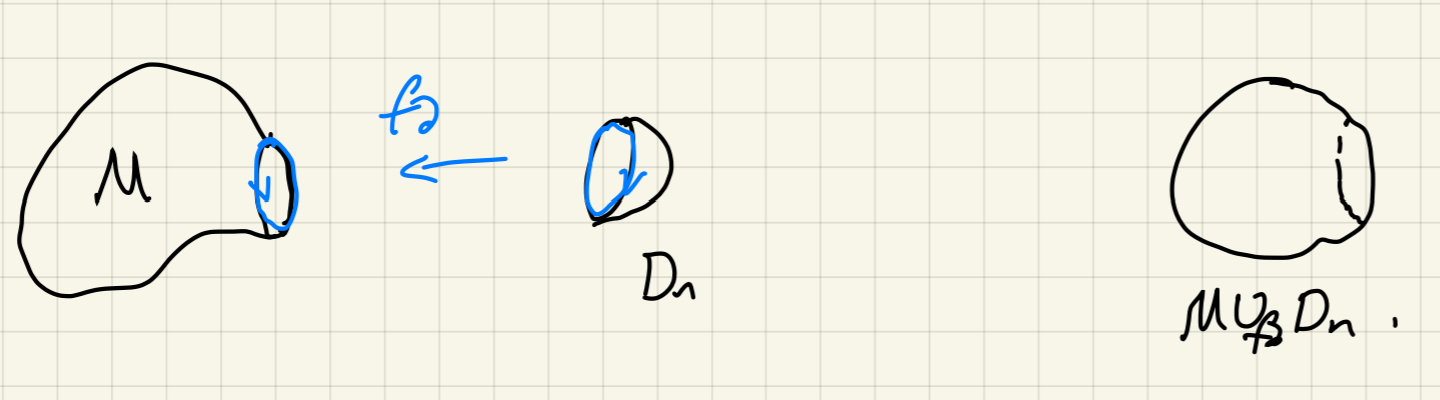
\includegraphics[width = 0.5\textwidth]{AttachingMap.png}
\end{center} 

\begin{exmp}
     $\man = \{p\}$ and $f_\partial : S^0 = \partial D_1 = \partial \inter \to \{p\}.$ Then $\man \cup_{f_\partial}D_1 = S^1$.
\end{exmp}

\begin{exercise}
    Show that if $\man$ admits a cell decomposition then so does $\man \cup_{f_\partial} D_n$.
\end{exercise}

\begin{exmp}
    $T = S^1 \times S^1 \subseteq \Real^3$. Let $f:T\to \Real:(x,y,z)\mapsto z$ be the height function. $\{c,b,a,0\}$ are critical points of $f$.
    \begin{center}
        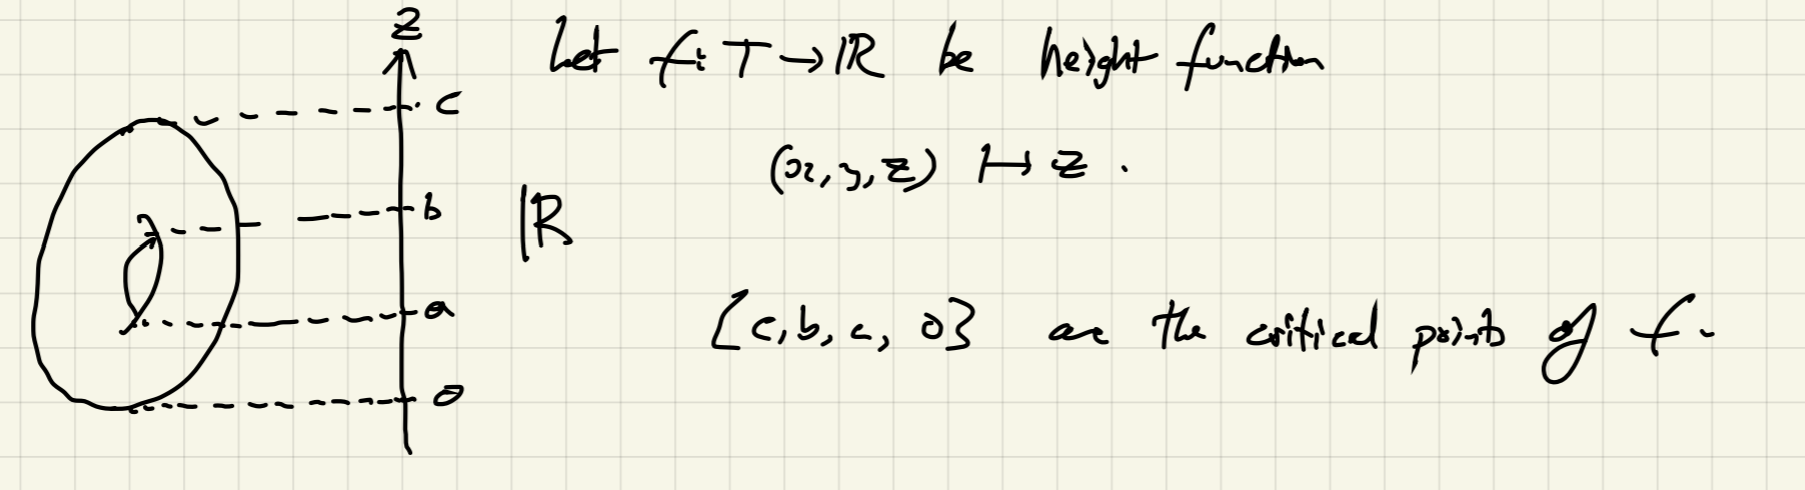
\includegraphics[width=0.5\textwidth]{TorusCellDecomposition.png}
    \end{center}
    Define $S_h \coloneqq \{p\in\man : f(p) \leq h\} = f^{-1}([0,h]), $ for $h\geq 0$. If $0<h<a$, then $S_h$ is homotopy equivalent to a 0-cell.
    \begin{center}
        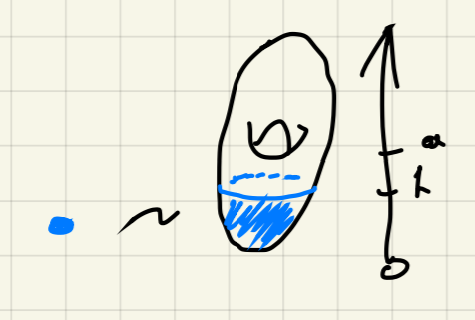
\includegraphics[width=0.25\textwidth]{MorseTorusTrivialHomotopy.png}
    \end{center}
    If $a<h<b$, then $S_h$ is homotopy equivalent to:    
    \begin{center}
        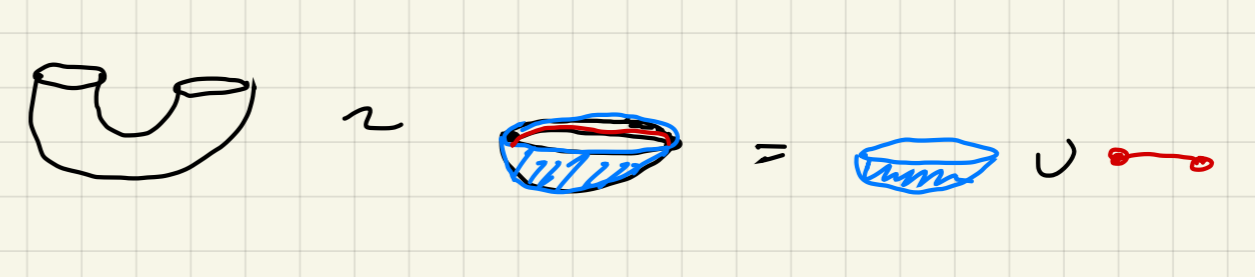
\includegraphics[width=0.5\textwidth]{MorseTorusHomotopyOneCell.png}
    \end{center}
    If $b<h<c$ then $S_h$ homotopy equivalent to:
    \begin{center}
        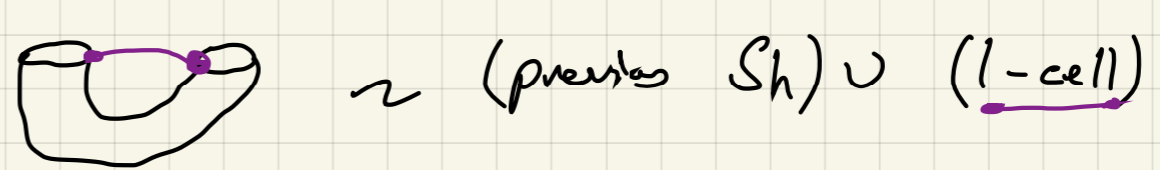
\includegraphics[width = 0.5\textwidth]{MorseTorusHomotopyOneCellWithZeroCell.png}
    \end{center}
    If $h>c$ then $S_h$ is homotopy equivalent to:
    \begin{center}
        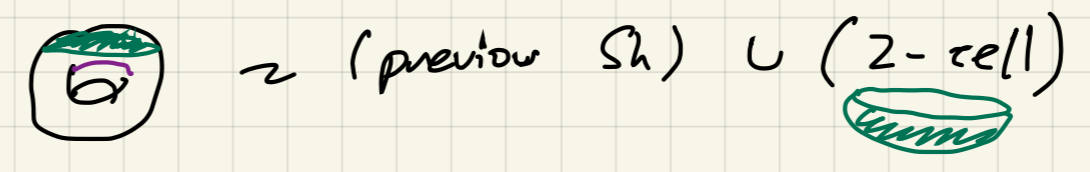
\includegraphics[width=0.5\textwidth]{MorseTorusHomotopyFullTorus.png}
    \end{center}
    Thus $\man$ = (0-cell)$\cup$(two 1-cells)$\cup$(2-cell).
\end{exmp}
Given a Morse function $f : \man \to \Real$ on a manifold $\man$, the idea is to study level sets $S_h = f^{-1}([-\infty,h]),$ and this will help us split up the manifold into manageable bits/cells.

\begin{defn}
    Let $f:\man \to\Real$ be a Morse function and $\xman$ be a critical point. Write $\Eig^-(H_f(x)) = \langle $eigenvectors of $H_f$ having negative eigenvalues$\rangle$. The \textbf{index} of $f$ at $x$ is the dimension of $\Eig^-H_f(x)$. ``This is something to do with the curvature properties of $f$ at the critical point''.
\end{defn}

\begin{lemma}[Morse Lemma]\label{lem:MorseLemma}
    Let $\man$ be a manifold of dimension $n$, $f:\man \to \Real$ a Morse function, $x_0 \in \man$ a critical point. Then there exists local coordinates ($x_1,\ldots,x_n)$ around $x_0$ s.t. $x_0 = (0,\ldots,0)$ and 
    $$f(x) = f(x_0) - \sumfromto{i=1}{\lambda} x_i^2 + \sumfromto{i=\lambda+1}{n} x_i^2$$
    where $\lambda$ is the index of $f$ at $x.$
\end{lemma}
``It can be proved in an elementary way I think, but the proof is quite long and not particularly enlightening'' (it's quite linear algebra-y but essentially relies on diagonalising the Hessian). See Copenhagen Lecture Notes (Cohen, Iga, Norbury 2009), Theorem 5.3 for a full proof.

\begin{corollary}
    The set of critical points of a Morse function is discrete.
\end{corollary}\noindent
This corollary is ``hugely important for Morse functions, and part of the reason we make the definition [of Morse functions] the way that we do.''

\begin{exercise}
    Check that $f$ as above has index $\lambda$ at $x_0$.
\end{exercise}

\begin{exmp}
    $f:\man \to \Real$ as before, $\man = S^1 \times S^1$. Blue is a negative eigenspace and red is a positive eigenspace in this drawing.
    \begin{center}
        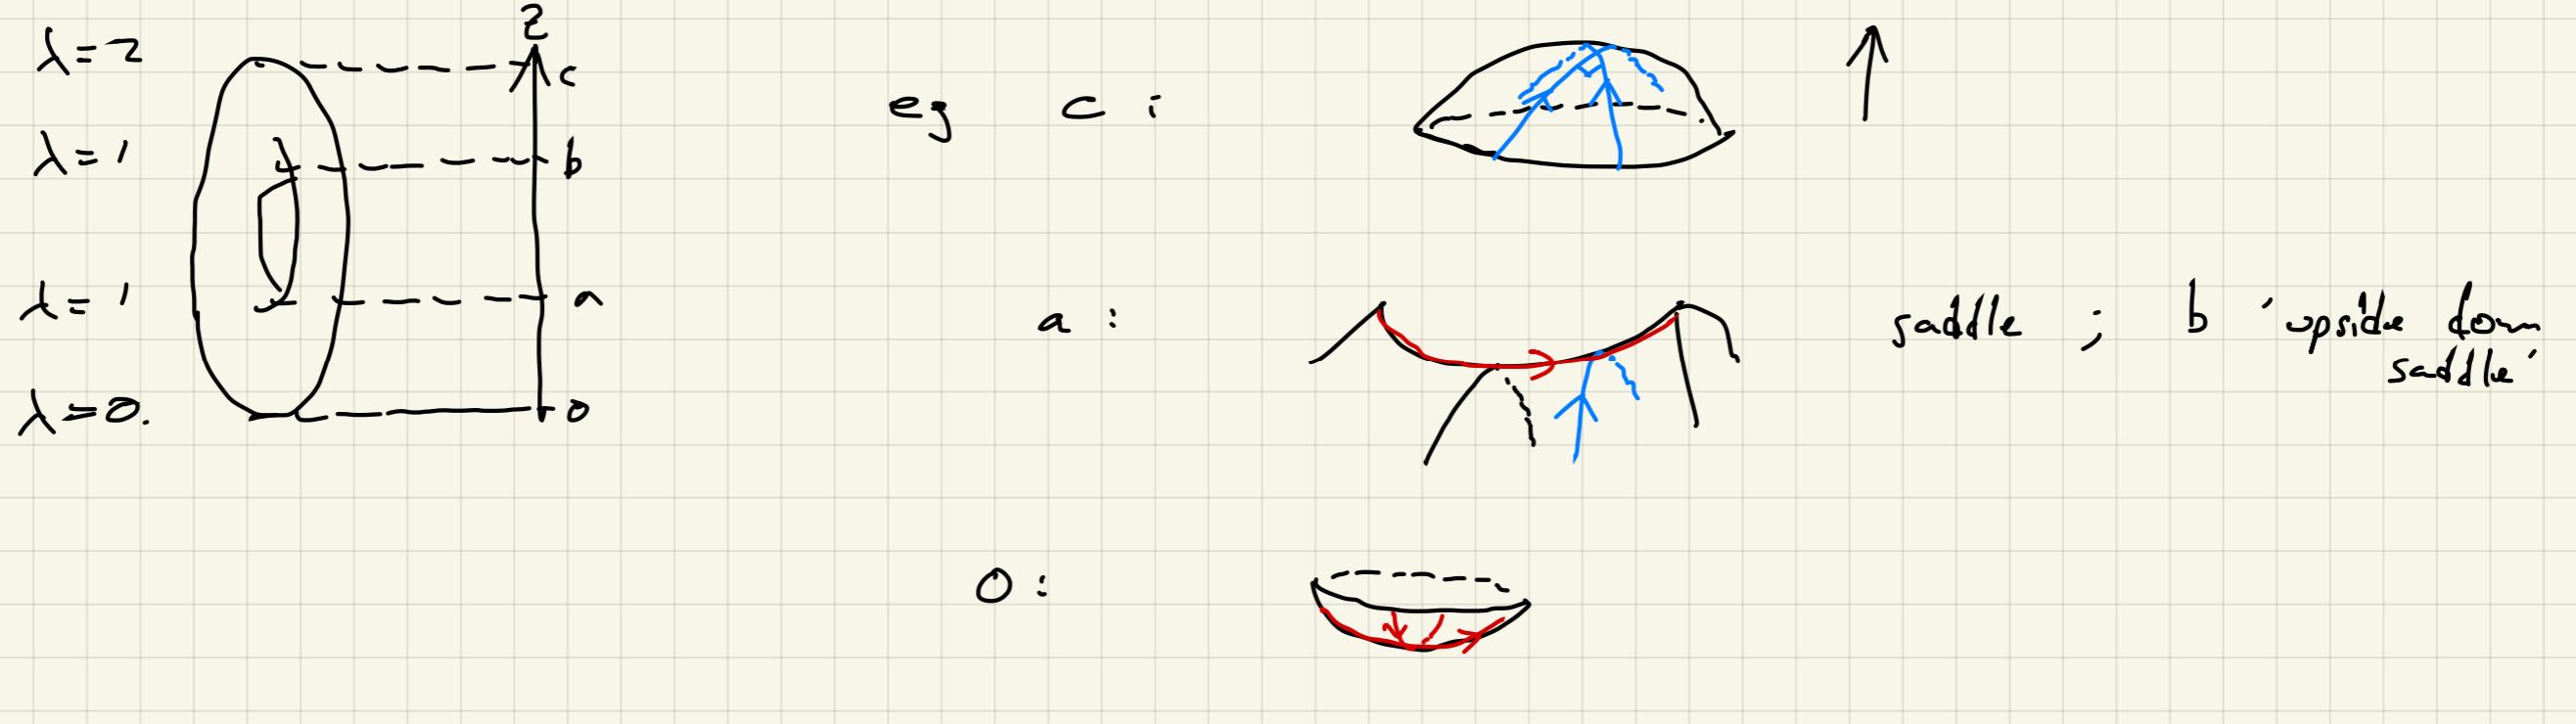
\includegraphics[width=\textwidth]{MorseTorusEigenvalues.png}
    \end{center}
\end{exmp}

\begin{subsection}{CW Complexes}
For a more detailed view on this topic see Hatcher, Algebraic Topology, Chapter 0.

\begin{defn}
    A topological space $\man$ admits a CW structure if there exists a sequence of topological subspaces $\man^{(0)} \subset \man^{(1)}  \subset \ldots \subset \man^{(n)}$ s.t.
    \begin{enumerate}
        \item $\man^{(0)}$ is a discrete subset of $\man$
        \item $\man^{(k)}$ is obtained from $\man^{(k-1)}$ by attaching $k$-cells
        \item $V\subset \man$ is closed iff $V\cap \man^{(k)}$ is closed for all $k$
    \end{enumerate}
    Such a $\man$ is called a CW complex. We say $\man$ is a finite CW complex iff it is obtained from attaching only finitely many cells. A subcomplex is a closed subspace of $\man$ which is a union of a subset of cells of $\man$. A closed cell is the image of $D_n$ in a cell. An open cell is the image of $D_n\backslash \partial D_n$ in a cell (NB: Open cells are not in general open in $\man$ e.g. an $n-1$ dimensional open cell in an $n$ dimensional manifold is not open wrt that manifold).
\end{defn}
\noindent
So these are both structures you can put on topological spaces, as well as a kind of inductively-built topological space itself which is particularly nice. Not every topological space admits a CW complex.\\
\Fact If $n\neq 4$, then a manifold of dimension $n$ is a CW complex. If $n=4,$ then this is an open problem\footnote{``There's something particularly strange about 4 dimensional manifolds. Somehow manifolds of higher dimension seem to be easier to understand, and manifolds of lower dimensions are sort of somehow simple enough that you can hope to understand them. But dimension 4 is tricky, tricky for some reason.''}
\begin{exmp}
    \begin{itemize}
        \item $S^n = \{p\}\cup D_n = \man^{(0)}\cup \man^{(n)}$
        \item $\man = \Real^n$ and $\Lambda = \{$integral points of $\Real^n\} =\mathbb{Z}^n$ then $\Lambda$ gives a decomposition of $\Real^n$ into $n$-cubes, which are $n$-cells, where 0-cells are points of $\Lambda$, 1-cells are edges joining points of $\Lambda$ etc.
    \end{itemize}
\end{exmp}

\begin{prop}
   Let $\man$ be a CW complex. Then:
   \begin{enumerate}
       \item If $K\subset \man$ is compact, then it is contained in a finite union of open cells.
       \item The closure of every cell is contained in a finite subcomplex of $\man$ (This is a kind of local finiteness property).
   \end{enumerate}
\end{prop}

\begin{proof}
   1: Let $K\subset \man$ compact. Assume there exists infinitely many open cells having nonempty intersection with $K$. So there exists infinite sequence of points $S \coloneqq \{x_i\}\subset K$ lying in distinct open cells. We claim that $S\cap M^{(n)}$ is closed and discrete for all $n\geq 0$. For $n=0$ this is true, as $\man^{(0)}$ is discrete. Assume true for $n-1$. Then if $\{e_j\}$ are the $n$-cells, then the open cell corresponding to $e_j$ contains at most one point of $S$ (by construction of $S$). Thus $S\cap (\bigcup_j e_j)$ is closed and discrete. So $S\cap \man^{(n)}$ is closed and discrete. Since $S \subset K$ and $K$ is compact, it follows that $S$ is finite. \\
   2: Induct on the dimension of the cell. For $n=0$, this is true. Assume true for all $m\leq n-1$, and let $e_n$ be an $n$-cell. The border of $e_n$ is the image of $S^{n-1}$, so it is compact. Hence by 1., it is contained in a finite union of open cells of dimension smaller than $n$. By induction, each of these cells is contained in a finite subcomplex. The union of all of these is a finite subcomplex containing the border of $e_n$. Hence attaching $e_n$ we get a finite subcomplex containing $e_n$.
\end{proof}

\begin{corollary}
    Let $\man$ be a CW complex. Then any compact subset $K\subset man$ is contained in a finite subcomplex.
\end{corollary}

\begin{proof}
    The result follows from the above proposition since the union of finite subcomplexes is a finite subcomplex.
\end{proof}
That's everything on CW complexes. Next time we will be defining gradient flows and making a move towards defining Morse homology.
\end{subsection}
\end{section}

\begin{section}{Lecture 20: Gradient Flows}
``If you have a compact manifold with a Morse function then all of the gradient flow lines for the Morse function begin and end at critical points.'' This lecture will set up the foundations for this concept and also for Morse homology. This will be Mastery material for this course (may be included at the end or in series), but this lecture will make sense of some of the critical theorems in Morse theory which will be important outside of the Mastery questions. %tk%
\begin{defn}
    Let $\man$ be a manifold. A \textbf{flow} or a group of diffeomorphisms of $\man$ is a collection of diffeomorphisms $\varphi_t : \man \to \man$ for $t\in \Real \st $there exists $\varphi:\Real \times \man \to \man $ with $\varphi_t = \varphi(t , . )$, $\varphi_0 = \id_\man$ and $\varphi_s \circ \varphi_t = \varphi_{s+t}$.\\
    The flow line or \textbf{integral curve} for the flow $\varphi$ (given $\xman$) is $\gamma_x : \Real \to \man : t \mapsto \varphi(t,x)$ where $\gamma_x(0) = x$. Since $\frac{\deriv}{\dt} \gamma_x \restrict{t=0} \in \tang$, the flow defines a vector field on $\man$ i.e. a smooth section of $T\man$.
\end{defn}
On the other hand, given a vector field, can we produce an integral curve that corresponds to it? This corresponds to solving some system of differential equations, which we can do at least in some neighbourhood of $t=0$\footnote{See: Lee, Intro to Smooth Manifolds, Chapter 9}. 

\begin{lemma}
    Let $X$ be compactly supported on $\man$. Then $X$ generates a group of diffeomorphisms $\varphi_t : \man \to \man$ such that we have $$(X\circ \gamma_x)(t) = \frac{\deriv}{\dt}\gamma_x(t),\; \xman$$
    We can show that flow lines are disjoint, so this decomposes/partitions $\man$ into a disjoint union of flow lines.
\end{lemma}

\begin{exmp}
    Let $\man = \Real$ and $X = x^2 \parderiv{x}$. What is the flow? (Solution is $\gamma_x(t) = \frac{\gamma_x(0)}{\gamma_x(0) t + 1})$
\end{exmp}

\begin{defn}
    A $\textbf{Riemannian metric}$ on a manifold $\man$ is a collection of inner products on  each $\tang$. given by $g_x:\tang\times\tang \to \Real$ such that for all vector fields $X \myand Y$ we have that $g_x(X(x),Y(x)): \man \to \Real$ is smooth. A \textbf{Riemannaian manifold} ($\man,g)$ is a manifold equipped with a Riemannian metric. ``Intutitively a way of measuring distance on a manifold.''
\end{defn}
Important consequence: $g$ gives an isomorphism $\tangbundle \cong \Omega^1(\man) = (\tangbundle)^*$ i.e. given $V$ a vector space with an inner product $\langle . , .\rangle$, we have an isomorphism $V\to V^*$ given by $v\mapsto \langle v, .\rangle$. ``This is something that is perhaps is easy to overlook the importance of.'' It kind of lets us easily choose dual bases, which we just did easily because there is a canonical inner product on $\Real^n$ once you have chosen coordinates. This choice of coordinates is `secretly' a choice of Riemannian metric on $\Real^n$, but this choice can be generalised as you will see if you study Riemannian Geometry. For our purposes, we will just be using metric spaces to define the gradient vector field. 

\begin{defn}
    Let $(\man,g)$ be a Riemannian manifold, and $f:\man\to\Real$ a smooth function. Then the \textbf{gradient vector field} $\nabla f$ of $f$ is the unique vector field on $\man$ s.t. for all vector fields $X$, $g(\nabla f, X) = Df(X)$.
\end{defn}
The isomorphism $\tangbundle \cong \Omega^1(\man)$ is what allows us to prove that this vector field exists and is unique. So the gradient vector field is the vector field that is dual to the differential of $f$ wrt $g$.
\Note $g(\nabla f,\nabla f) = \norm{\nabla f}^2 = Df(\nabla f),$ so $\nabla f(x) = 0 $ iff $x$ is a critical point of $f$.\\
\Note $\nabla f$ is orthogonal to any vector tangent to $f^{-1}(c)$ for all regular values $c\in\Real.$\\
This really is just a generalisation of the usual $\nabla f$ from real multivariate calculus and works in the way that you would expect: it points in the direction of greatest change of $f$, orthogonal to lines where the value of $f$ is constant. In particular, we can take the flow associated to $-\nabla f$ for a smooth function $f:\man \to \Real $ i.e.: 
\begin{defn}
    If $\gamma_x(t) = \varphi(t,x)$ the $\frac{\deriv}{\dt} \gamma_x(0)\restrict{t=0} = -\nabla f(\gamma_x(0)), \, \gamma_x(0) = x$. This is called the \textbf{gradient flow} of $f$. The integral curves are called gradient flow lines.
\end{defn}
Imagine these flow lines as the paths of particles of water if you poured some on the manifold (if $f$ is the height function anyway). Most will flow onto the very bottom critical point, but there are some special points where it will flow onto a critical point where it will remain in equilibrium.
\begin{center}
    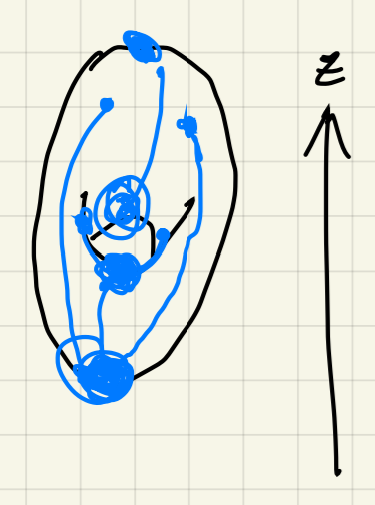
\includegraphics[width = 0.20\textwidth]{WaterGradientFlowLines.png}
\end{center}
``So we get some sort of decomposition of our manifold by asking: Which critical point do you flow down to? And that's the decomposition that Morse homology is concerned with.''

\begin{lemma}
    $f$ decreases along gradient flow lines, i.e. $f(\gamma_x(t)):\Real \to \Real$ is a decreasing function of $t\in\Real$.
\end{lemma}
\begin{proof}
    $\tdiffof{} f(\gamma_x(t)) = Df_{\gamma_x(t)} (\tdiffof{} \gamma_x(t)) = Df_{\gamma_x(t)}(- \nabla f(\gamma_x(t))) = - \norm{\nabla f(\gamma_x(t))}^2 \leq 0$
\end{proof}

\begin{prop}
   Let $\man$ be compact with $f:\man\to\Real$ Morse function. Then every gradient flow line begins and ends at a critical point i.e. $\lim \limits_{t \to \pm \infty} \gamma_x(t) $ exist and are critical points of $f$.
\end{prop}

\begin{proof}
    First assume the limits exist. For all $x$, $f(\gamma_x(t)) : \Real \to \Real$ is bounded because $\man$ is compact. Then $\lim \limits_{t \to \pm \infty} \tdiffof{} f(\gamma_x(t)) = \lim \limits_{t \to \pm \infty} - \norm{\nabla f(\gamma_x(t))}^2$. And $\lim \limits_{t \to \pm \infty} \tdiffof{}f(\gamma_x(t)) = 0$ because $f$ is bounded and decreasing along flow lines. So the limit is a critical point if it exists.\\
    Now we show it exists. Fix $\epsilon> 0$ and let $U $ be the union of open balls of radius $\epsilon$ around each critical point of $f.$ Since $\man$ is compact and $f$ is Morse, there are only finitely many critical points. Then $U$ is open, so $\man \backslash U$ is closed, so $\man \backslash U$ is compact, so $\norm{\nabla f(.)}^2$ admits a minimum in $\man \backslash U$. But this minimum cannot be zero because we removed all the critical points. But $\lim \limits_{t \to \pm \infty}\norm{\nabla f(\gamma_x(t))}^2 = 0$ because $f(\gamma_x(t))$ is bounded and decreasing. So if $\pm t$ is large enough, then $\gamma_x(t) \not\in \man \backslash U$, so if $\epsilon $ sufficiently small, $\gamma_x(t)$ is contained in a ball around a single critical point for $t \to \pm$. Thus the limit is the critical point. 
\end{proof}
The rest of the Morse theory material is Mastery material. Outside of that, next time we will be switching gears and talking about singular homology and singular cohomology. At the end of the course we will be proving the de Rham theorem, showing how singular cohomology and de Rham cohomology are the same.

\end{section}











\end{document}
%%%%%%%%%%%%%%%%%%%%%%%%%%%%%%%%%%%%%%%%%%%%%%